%
% TU/e Style Master Thesis template for LaTeX
%
% Public version 1.0
% 2010 - 2013 Thijs Nugteren and Joos Buijs
	%
% THIS IS THE MAIN FILE (i.e. compile this file, compiling the others directly won't work)
%
\documentclass[a4paper,12pt,twoside]{report}

%all the other includes etc. are done in the thesis.sty file.
\usepackage{thesis}
\usepackage[authoryear]{natbib}
\makenomenclature
\definecolor{mygray}{gray}{0.9}
%
% These commands need to be defined in order to produce a correct nad personalized document
%
\newcommand{\shortdoctitle}{PhD T
hesis}
\newcommand{\doctitle}{Report}
\newcommand{\docsubtitle}{Mid-term}

\newcommand{\me}{MIRA Anna}
\newcommand{\keywords}{Breast mechanics,FEM, Mammography}
\newcommand{\version}{V1}
\newcommand{\monthYear}{September 2016}

%Be sure to use all the titles for your committee members!!! (their names show up on the very first page!)
\newcommand{\firstCommitteeMember}{ Yohan Payan, TIMC-IMAG Lab, CNRS \& Univ. Grenoble Alpes}
\newcommand{\secondCommitteeMember}{Serge Muller, GE-Healthcare, France}
\newcommand{\thirdCommitteeMember}{Ann-Katherine Carton, GE-Healthcare, France}

\author{\me}

%
% PDF settings
%
\hypersetup
{
    pdfauthor={\me},
    pdftitle={\shortdoctitle},
    pdfsubject={\doctitle},
    pdfkeywords={\keywords}
}

\setlength\aftertitleunit{\baselineskip}

\titleformat{\chapter}[display]
  {\normalfont\huge\bfseries}{}{0pt}{\Huge}
\titleformat{name=\chapter,numberless}[display]
  {\normalfont\huge\bfseries}{}{0pt}{\Huge}
\titlespacing*{\chapter}{0pt}{50pt}{*2}



\begin{document}

%use this include for PDF and distribution versions
\pagenumbering{roman}
\begin{titlepage}
%
\includegraphics[height=2cm]{figures/univGrenobleAlpes.jpg}\\
%\LARGE
%Eindhoven University of Technology \\
%\LARGE Universit\'e Grenoble Alpes
%\vspace*{10cm}

\setlength{\TPHorizModule}{1mm}
\setlength{\TPVertModule}{\TPHorizModule}
% Set the Paragraph Indent to zero, so the first line is not Indented
% Back-up the current value so it can be put back at the end of the title page
\newlength{\backupparindent}
\setlength{\backupparindent}{\parindent}
\setlength{\parindent}{0mm}			
% Begins a textbox at 72 mm from the left of the edge of the paper and 89 mm from the top
% The width of the textbox is 95 mm (167 - 72 mm)
% The height of the box cannot be defined, so it is your task to keep the text not too long
\begin{textblock}{167}(25,89)
    \vspace*{1mm}
    \huge
    \textbf{\doctitle \\}
    \Large
    \vspace*{5mm}
    \textit{\docsubtitle}\\
    \vspace*{10mm}
    \Large
    \me\\
\end{textblock}

\begin{textblock}{167}(25,150)
	\Large
	Supervised by: \\
    \hspace*{5cm}\firstSupervisor\\
     \hspace*{5cm}\secondSupervisor\\
     \hspace*{5cm}\thirdSupervisor\\
     
     \vspace*{1cm}
     Jury members:\\
     \hspace*{5cm}\firstCommitteeMember\\
	 \hspace*{5cm}\secondCommitteeMember\\
	 

\end{textblock}

%\version
\mbox{~} % ou tout simplement l'espace insécable ~ mais on risque de l'oublier. 
\vfill 
\begin{center}
\large
Defense \monthYear\\
\end{center}
%\docdate \\

% Put the Paragraph Indent back to its original value
\setlength{\parindent}{\backupparindent}

\end{titlepage} 

\normalsize

\clearemptydoublepage

%Sometimes line numbers are nice, uncomment the next line to enable:
\linenumbers

%It could be handy to have a list of todos and brainstorms in your thesis
%\chapter*{*General todos*}\todo{remove this chapter}
%\input{chapters/general_todos}



\tableofcontents

\clearemptydoublepage

\listoffigures

\clearemptydoublepage

\listoftables

\clearemptydoublepage
% Generate the glossary
\printnomenclature
\clearemptydoublepage

%\lstlistoflistings

%\clearemptydoublepage

%\chapter{Introduction}\label{chapter:introduction}
\setcounter{page}{0}
\pagenumbering{arabic}
%from here on, start the 'real' page numbering, from 1, with normal digits
%\chapter*{General problem statement}
\label{section:generalproblemstatment}
\markboth{\textsc{General problem statement}}{}
\addcontentsline{toc}{chapter}{General Problem statement}

Today, mammography is the primary imaging modality for breast cancer screening and plays an important role in cancer diagnosis. Subtle soft-tissue findings and microcalcifications that may represent early breast cancer are visualized by means of X-rays images. After investigation, the abnormal findings are taken in charge for further evaluation.  

A standard mammography protocol always includes breast compression prior to image acquisition. Women breast is compressed between two plates until a nearly uniform breast thickness is obtained. The breast flattening improves diagnostic image quality and reduces the absorbed dose of ionizing photons. However, the discomfort and pain induced by this compression procedure might deter women from attending a mammography. Fleming et al. \citep{fleming_intermittent_2013} showed in a 2500 women panel study that 15\% of those who skipped the second appointment cited an unpleasant or painful first mammogram.  

An important improvement concerning the patient comfort could be achieved with the emergence of Full-Field Digital Mammography (FFDM). Due to the improved detector capabilities, digital mammography became better in terms of image quality and radiation dose than Film–Screen Mammography. The use of Automatic Exposure Control (AEC) allowed to estimate the acquisition parameters providing the optimal image quality and average glandular dose for a given breast thickness and glandularity. Therefore, FFDM may reduce breast compression while respecting the clinical gold standards on image quality.

Subsequently, there is an opportunity to leverage the potential of the recent imaging technologies by developing alternative breast compression techniques. The new techniques have to consider the patient comfort in addition to an improved image quality and a reduced ionizing radiation dose. This may imply another paddle geometry or peculiar material properties as well as distinct compression paddle positioning.

The goal of this PhD thesis was to develop a simulation environment able to characterize the impact of the paddle design on the patient comfort and its repercussion on the mammography image quality and average glandular dose. Due to the complexity of in-vivo clinical studies, a realistic simulation framework is of a large interest. To this end, the following tasks were considered.
\begin{itemize}
\item To develop a biomechanical breast model taking into consideration the subject-specific breast geometry and tissues' mechanical properties. 

\item To evaluate this biomechanical breast model. 

\item To model the breast deformations under compression.

\item To integrate the corresponding deformable breast phantom into the image acquisition simulation framework.
\item To compute compression quality measures able to characterize the differences between various breast compression techniques in terms of patient comfort, image quality and average glandular dose.  

\end{itemize}   

Using the developed tools, two studies could be performed.
\begin{itemize}
\item To assess the differences between standard rigid and flex paddles in terms of patient comfort, image quality and average glandular dose for two different breast volumes.

\item To assess the breast positioning impact on compression mechanics and patient comfort, considering one breast volume and one paddle model.
\end{itemize}
 
\cleardoublepage
\chapter*{Technical approach}\label{section:technicalapproach}
\addcontentsline{toc}{chapter}{Technical approach}
\markboth{\textsc{Technical approach}}{}

To study the impact of the paddle design on the compression quality, a simulation framework was developed.  The breast mechanics and patient comfort were addressed by the means of finite element modeling (ANSYS\footnote{https://www.ansys.com/}). On the other hand, the image quality could be assessed by using an image simulation framework modeling the X-rays propagation trough matter during acquisition of a mammography image (CatSim\footnote{Milioni de Carvalho P. 2014, PhD thesis}). 

First, to develop a subject-specific breast model, the MR images of two volunteers in three distinct positions (supine,prone and supine tilted) were acquired. The MRI volumes were processed (ITK\footnote{https://itk.org/}/ VTK\footnote{https://www.vtk.org/}/ CamiTK\footnote{http://camitk.imag.fr/}) and segmented (ITK-Snap\footnote{http://www.itksnap.org}). Then, the processed images were used to extract the 3D surfaces of the breast, compatible with ANSYS Mechanical meshing software. The breast geometries was discretized using tetrahedral solid elements and were the subjects of hyper-elastic quasi-static simulations. An exhaustive optimization process was performed to determine the subject-specific tissues mechanical properties as well as the corresponding breast stress-free configuration. The model was developed and calibrated such as the best estimates of supine and prone breast configurations were obtained. The model accuracy was assessed in terms of Hausdorff distance between the measured and estimated breast surfaces in supine tilted configuration.

Once the model was created and evaluated, it was used to quantify the breast compression quality. To this end, different finite element models of the paddle were developed with peculiar assumption on their flexibility and degrees of freedom. For each simulation of breast compression, the patient comfort was associated with the internal tissues stress/strain distribution and the pressure range at the skin surface. The mean average dose was computed using the model proposed by Dance et al. \cite{dance_additional_2000} for the corresponding breast thickness was derived from finite element simulations. The compressed breast geometry was then imported into the image simulation software (CatSim) together with an embedded set of virtual microcalcifications. Synthetic projections were then generated and the signal to noise ratio as well as the signal-difference to noise ratio were computed to characterize the resulting image quality.   

\cleardoublepage
\chapter*{Thesis overview}\label{section:thesisoverview}
\addcontentsline{toc}{chapter}{Thesis overview}
\markboth{\textsc{Thesis overview}}{}

This manuscript is divided into six major chapters.  \textbf{Chapter \ref{chapter:clinicalbachground}}, describes the clinical background  required for a good understanding of our work. Both internal and external structure of the breast are described. The role of regular screening for breast cancer is discussed with a list of involved medical imaging technologies. 

Chapters 2 and 3 are focused on breast biomechanical modeling. \textbf{Chapter \ref{chapter:bioMecaModelsBackground}} provides a brief introduction to the continuous and contact mechanics and describes the finite element numerical method able to solve such problems.  This chapter provides also a review on biomechanical modeling of the breast. Successes and failures of experiments reported in the literature, to determine the tissues material properties and breast stress-free geometry, are discussed. The most advanced biomechanical models are listed with their corresponding errors with reference to real breast deformations. \textbf{Chapter \ref{chapter:myBioMecaModel}} describes the breast biomechanical model we have proposed and the multi-loading gravity simulations that we performed to evaluate the model. First, the patient data acquisition as well as the required image pre-processing operations are presented. The optimal mesh size for such simulations is determined. Then, the model sensitivity to different boundary conditions and constitutive parameters is studied. The best modeling techniques of the main anatomical structures, such as the suspensory ligaments and the pectoral fascia, are selected. The results of the optimization process allowing to estimate the subject specific mechanical properties of breast tissues and stress-free geometry are presented.
Finally, the model fidelity to the real deformations, as measured in MR images of the breast in three different configurations, is discussed.

Chapters 4 and 5 are focused in breast deformation under compression modeling, as well as on the assessment of the compression quality in mammography. \textbf{Chapter \ref{chapter:compression:introduction}} describes the breast compression process and its associated mechanics as recorded during real mammography acquisitions. The role of tissues compression in mammography as well as the current gold standards for image quality and average glandular dose are discussed. The last proposed technologies dealing with patient comfort and pain reducing techniques are outlined with their impact on patient comfort. In \textbf{Chapter \ref{chapter:compressionfem}}, two studies on breast compression quality are described. First, the finite element models of standard compression paddles are provided with the corresponding assumptions on their dynamics. The computed compression force and breast thickness are compared to the corresponding parameters issued from real mammography exams underwent by the volunteers. The derived adjustments of tissues constitutive models are provided. The details for mammography images simulation and breast phantom creation are also discussed. Next, the metrics of image quality, average glandular dose and patient comfort are defined and used to compare the compression quality between different paddle models and different paddle positions. 
 
Finally, \textbf{Chapter \ref{section:generalconclusion}} summarizes the work reported on this manuscript and generalizes the corresponding results. Perspectives and directions for future work are also provided.  

\cleardoublepage  

\chapter*{Ethics and Funding}\label{section:ethics}
\addcontentsline{toc}{chapter}{Ethics}
\markboth{\textsc{Ethics and Funding}}{}

This research project is financially supported by ANRT, CIFRE n°2014/1357.
\\

\noindent
The two involved volunteers agreed to participate in a pilot study approved by an ethical committee, MammoBio MAP-VS pilot study.
% We are thanking the \textbf{IRMaGe} MRI facility (Grenoble,France) for their participation in image data acquisition. 

\cleardoublepage


%\clearemptydoublepage
%\chapter{Preliminaries}\label{chapter:preliminaries}

\clearemptydoublepage


\part{Introduction}\label{chapter:introduction}
\chapter*{General problem statement}
\label{section:generalproblemstatment}
\markboth{\textsc{General problem statement}}{}
\addcontentsline{toc}{chapter}{General Problem statement}

Today, mammography is the primary imaging modality for breast cancer screening and plays an important role in cancer diagnosis. Subtle soft-tissue findings and microcalcifications that may represent early breast cancer are visualized by means of X-rays images. After investigation, the abnormal findings are taken in charge for further evaluation.  

A standard mammography protocol always includes breast compression prior to image acquisition. Women breast is compressed between two plates until a nearly uniform breast thickness is obtained. The breast flattening improves diagnostic image quality and reduces the absorbed dose of ionizing photons. However, the discomfort and pain induced by this compression procedure might deter women from attending a mammography. Fleming et al. \citep{fleming_intermittent_2013} showed in a 2500 women panel study that 15\% of those who skipped the second appointment cited an unpleasant or painful first mammogram.  

An important improvement concerning the patient comfort could be achieved with the emergence of Full-Field Digital Mammography (FFDM). Due to the improved detector capabilities, digital mammography became better in terms of image quality and radiation dose than Film–Screen Mammography. The use of Automatic Exposure Control (AEC) allowed to estimate the acquisition parameters providing the optimal image quality and average glandular dose for a given breast thickness and glandularity. Therefore, FFDM may reduce breast compression while respecting the clinical gold standards on image quality.

Subsequently, there is an opportunity to leverage the potential of the recent imaging technologies by developing alternative breast compression techniques. The new techniques have to consider the patient comfort in addition to an improved image quality and a reduced ionizing radiation dose. This may imply another paddle geometry or peculiar material properties as well as distinct compression paddle positioning.

The goal of this PhD thesis was to develop a simulation environment able to characterize the impact of the paddle design on the patient comfort and its repercussion on the mammography image quality and average glandular dose. Due to the complexity of in-vivo clinical studies, a realistic simulation framework is of a large interest. To this end, the following tasks were considered.
\begin{itemize}
\item To develop a biomechanical breast model taking into consideration the subject-specific breast geometry and tissues' mechanical properties. 

\item To evaluate this biomechanical breast model. 

\item To model the breast deformations under compression.

\item To integrate the corresponding deformable breast phantom into the image acquisition simulation framework.
\item To compute compression quality measures able to characterize the differences between various breast compression techniques in terms of patient comfort, image quality and average glandular dose.  

\end{itemize}   

Using the developed tools, two studies could be performed.
\begin{itemize}
\item To assess the differences between standard rigid and flex paddles in terms of patient comfort, image quality and average glandular dose for two different breast volumes.

\item To assess the breast positioning impact on compression mechanics and patient comfort, considering one breast volume and one paddle model.
\end{itemize}
 
\cleardoublepage
\chapter*{Technical approach}\label{section:technicalapproach}
\addcontentsline{toc}{chapter}{Technical approach}
\markboth{\textsc{Technical approach}}{}

To study the impact of the paddle design on the compression quality, a simulation framework was developed.  The breast mechanics and patient comfort were addressed by the means of finite element modeling (ANSYS\footnote{https://www.ansys.com/}). On the other hand, the image quality could be assessed by using an image simulation framework modeling the X-rays propagation trough matter during acquisition of a mammography image (CatSim\footnote{Milioni de Carvalho P. 2014, PhD thesis}). 

First, to develop a subject-specific breast model, the MR images of two volunteers in three distinct positions (supine,prone and supine tilted) were acquired. The MRI volumes were processed (ITK\footnote{https://itk.org/}/ VTK\footnote{https://www.vtk.org/}/ CamiTK\footnote{http://camitk.imag.fr/}) and segmented (ITK-Snap\footnote{http://www.itksnap.org}). Then, the processed images were used to extract the 3D surfaces of the breast, compatible with ANSYS Mechanical meshing software. The breast geometries was discretized using tetrahedral solid elements and were the subjects of hyper-elastic quasi-static simulations. An exhaustive optimization process was performed to determine the subject-specific tissues mechanical properties as well as the corresponding breast stress-free configuration. The model was developed and calibrated such as the best estimates of supine and prone breast configurations were obtained. The model accuracy was assessed in terms of Hausdorff distance between the measured and estimated breast surfaces in supine tilted configuration.

Once the model was created and evaluated, it was used to quantify the breast compression quality. To this end, different finite element models of the paddle were developed with peculiar assumption on their flexibility and degrees of freedom. For each simulation of breast compression, the patient comfort was associated with the internal tissues stress/strain distribution and the pressure range at the skin surface. The mean average dose was computed using the model proposed by Dance et al. \cite{dance_additional_2000} for the corresponding breast thickness was derived from finite element simulations. The compressed breast geometry was then imported into the image simulation software (CatSim) together with an embedded set of virtual microcalcifications. Synthetic projections were then generated and the signal to noise ratio as well as the signal-difference to noise ratio were computed to characterize the resulting image quality.   

\cleardoublepage
\chapter*{Thesis overview}\label{section:thesisoverview}
\addcontentsline{toc}{chapter}{Thesis overview}
\markboth{\textsc{Thesis overview}}{}

This manuscript is divided into six major chapters.  \textbf{Chapter \ref{chapter:clinicalbachground}}, describes the clinical background  required for a good understanding of our work. Both internal and external structure of the breast are described. The role of regular screening for breast cancer is discussed with a list of involved medical imaging technologies. 

Chapters 2 and 3 are focused on breast biomechanical modeling. \textbf{Chapter \ref{chapter:bioMecaModelsBackground}} provides a brief introduction to the continuous and contact mechanics and describes the finite element numerical method able to solve such problems.  This chapter provides also a review on biomechanical modeling of the breast. Successes and failures of experiments reported in the literature, to determine the tissues material properties and breast stress-free geometry, are discussed. The most advanced biomechanical models are listed with their corresponding errors with reference to real breast deformations. \textbf{Chapter \ref{chapter:myBioMecaModel}} describes the breast biomechanical model we have proposed and the multi-loading gravity simulations that we performed to evaluate the model. First, the patient data acquisition as well as the required image pre-processing operations are presented. The optimal mesh size for such simulations is determined. Then, the model sensitivity to different boundary conditions and constitutive parameters is studied. The best modeling techniques of the main anatomical structures, such as the suspensory ligaments and the pectoral fascia, are selected. The results of the optimization process allowing to estimate the subject specific mechanical properties of breast tissues and stress-free geometry are presented.
Finally, the model fidelity to the real deformations, as measured in MR images of the breast in three different configurations, is discussed.

Chapters 4 and 5 are focused in breast deformation under compression modeling, as well as on the assessment of the compression quality in mammography. \textbf{Chapter \ref{chapter:compression:introduction}} describes the breast compression process and its associated mechanics as recorded during real mammography acquisitions. The role of tissues compression in mammography as well as the current gold standards for image quality and average glandular dose are discussed. The last proposed technologies dealing with patient comfort and pain reducing techniques are outlined with their impact on patient comfort. In \textbf{Chapter \ref{chapter:compressionfem}}, two studies on breast compression quality are described. First, the finite element models of standard compression paddles are provided with the corresponding assumptions on their dynamics. The computed compression force and breast thickness are compared to the corresponding parameters issued from real mammography exams underwent by the volunteers. The derived adjustments of tissues constitutive models are provided. The details for mammography images simulation and breast phantom creation are also discussed. Next, the metrics of image quality, average glandular dose and patient comfort are defined and used to compare the compression quality between different paddle models and different paddle positions. 
 
Finally, \textbf{Chapter \ref{section:generalconclusion}} summarizes the work reported on this manuscript and generalizes the corresponding results. Perspectives and directions for future work are also provided.  

\cleardoublepage  

\chapter*{Ethics and Funding}\label{section:ethics}
\addcontentsline{toc}{chapter}{Ethics}
\markboth{\textsc{Ethics and Funding}}{}

This research project is financially supported by ANRT, CIFRE n°2014/1357.
\\

\noindent
The two involved volunteers agreed to participate in a pilot study approved by an ethical committee, MammoBio MAP-VS pilot study.
% We are thanking the \textbf{IRMaGe} MRI facility (Grenoble,France) for their participation in image data acquisition. 

\cleardoublepage

%clinical background
\clearemptydoublepage
\part{Background}\label{part:background}
\chapter{ Clinical background}\label{chapter:clinicalbachground}

In France, in 2012, approximately 1.2 million new cases were diagnosed, and 400,000 women died from breast cancer. Early detection of cancer is a major condition to a fast and full recovery from breast cancer. Today, mammography is by far the primary imaging modality for breast cancer screening and plays an important role in cancer diagnosis. However, frequently this experience is described by women as unpleasant and sometimes painful.

The aim of this chapter is to provide the required clinical background on breast cancer screening and diagnosis for a good understanding of the global aim and relevance of the present work. 

First the breast evolution from early to the adult ages is described, with a detailed characterization of internal and external adult breast structures. To explain the intra-individual variation of breast mechanical and structural properties, the hormonal changes during the menstrual cycle, pregnancy or menopause are presented.   Next the cancer edogenesis is described and the most common types are characterized. Finally, different modalities for breast imaging are presented with their underlying technical principals as well as their utilization and relevance for breast cancer regular screening.

\clearpage
\section{Breast anatomy}\label{section:breastanatomy}

Internal and external breast structures will be repeatedly referenced in the following work, therefore their detailed description including mechanical properties and their localization is needed. Although the breast anatomy seems to be simple and easy to understand, a detailed analysis of breast embryogenesis is requested for a better localization the supporting breast tissues. The breast support matrix is a structure of high interests when modeling breast mechanics.  

  
\subsection{Breast embryogenesis}\label{subsection:breastembryogenesis}

The breast is a modified skin gland which starts to develop at the embryonic stage from the epidermis and dermis.  During the sixth fetal month, from 12 to 20 solid cords of epithelial cells are growing down into the dermis (Figure. \ref{breastembryogenesis}.a-b). Later, these cords evolve into lactiferous ducts and alveoli (fig. \ref{breastembryogenesis}.c-d). Thus, near birth, a simple network of branching ducts is already developed in the pectoral area \citep{skandalakis_embryology_2009}.
 

 \begin{figure}[!h]
 \centering
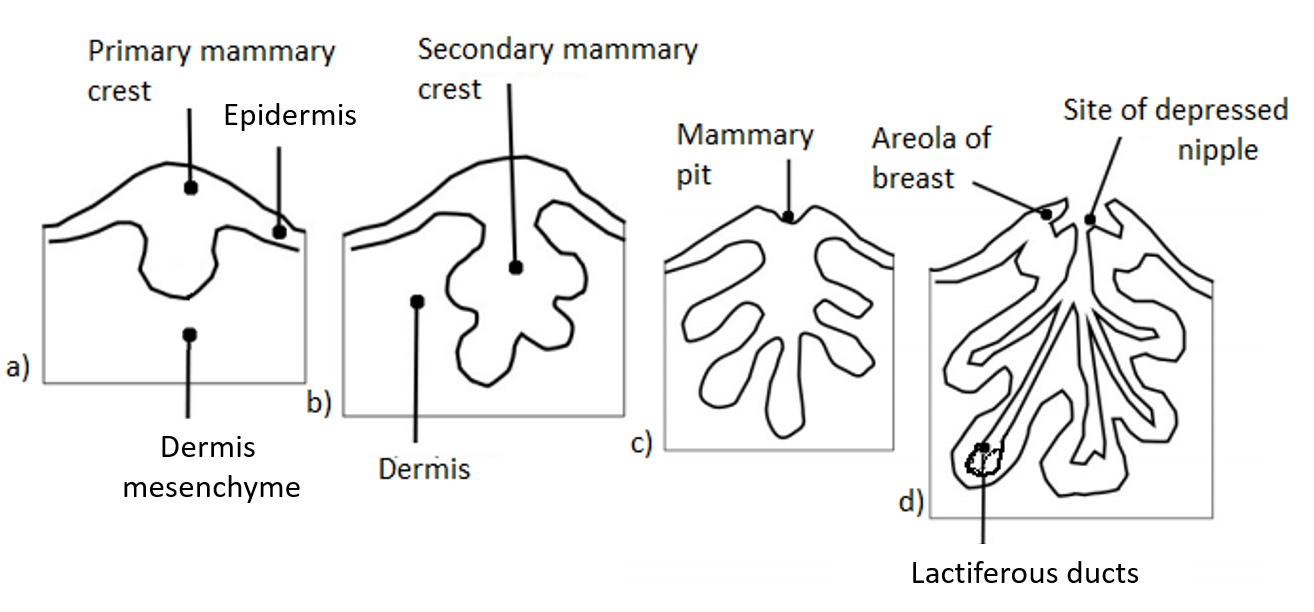
\includegraphics[width=0.8\textwidth,keepaspectratio]{figures/breast_evolution_my.png} 
\caption[Breast embryogenesis: embryonic evolution of duct system. The epidermis is responsible for the creation of ductal system and alveoli, the dermis mesenchyme is responsible for the creation of connective tissue and vessels] {Breast embryogenesism: stages of formation pf the duct system. the ectoderm is responsible for duct system and alveoli, the mesenchyme is responsible for the connective tissue and vessels \citep{skandalakis_embryology_2009}.}
\label{breastembryogenesis}
\end{figure}


The glandular lobes, generally remain underdeveloped until puberty (13 to 18 years). Under hormonal stimulation, the breast buds due to the development of the mammary glands and increased deposition of fatty tissues, becoming palpable discs beneath the nipple. The ducts grow into the soft tissues and the lobular differentiation begins \citep{kopans2007breast}. 

\cite{kopans2007breast} analyzed breast development sequence in the subcutaneous tissues. According to the authors the evolution of breast within the fascial system is unclear, with two possible evolution paths: 
\begin{enumerate}[label=(\Alph*)]
\item The superficial fascia splits in two layers forming the deep and the superficial fascia layers. The mammary glands appears between these two layers (Figure\ref{breastevol_fascia}.A).
\item The elongating ducts retracts the superficial fascia.  The mammary glands is enveloped by the superficial fascia (Figure\ref{breastevol_fascia}.B)
\end{enumerate}

\begin{figure}[!h]
\centering
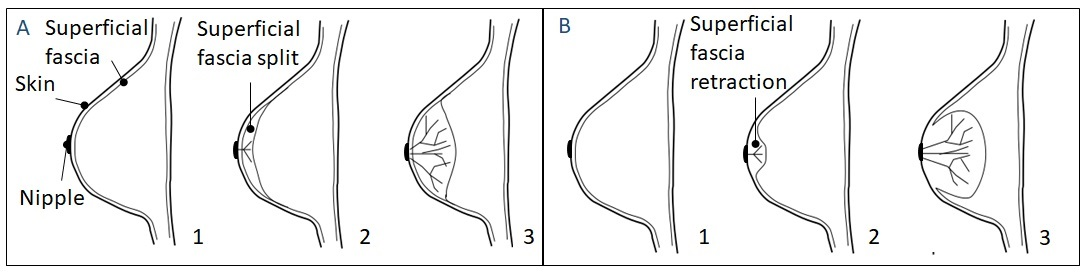
\includegraphics[width=0.9\linewidth,keepaspectratio]{figures/breastEvol_fascia_my.jpg} 
\caption[Breast development sequence into subcutaneous tissues. A Mammary bud development by splitting the superficial fascia in 2 layers. B Mammary bud development by superficial fascia retracting]{Breast development sequence in the subcutaneous tissues. A Mammary bud development by sleeting the superficial fascia in 2 layers. B Mammary bud development by fascia retracting, reproduced from  \citep{kopans2007breast}  }
\label{breastevol_fascia}
\end{figure}


\subsection{Breast external appearance}\label{subsection:breastappearance}

In order to describe the breast appearance, several notions for localization into the breast volume and its vicinity are defined. Usually, the breast volume is divided into four quadrants: upper outer quadrant (UOQ)\nomenclature{UOQ}{Upper Outer Quadrant}, upper inner quadrant (UIQ)\nomenclature{UIQ}{Upper Inner Quadrant}, lower outer quadrant (LOQ)\nomenclature{LOQ}{Lower Outer Quadrant}, lower inner quadrant (LIQ)\nomenclature{LIQ}{Lower Inner Quadrant}(see Figure\ref{fig:Breast_quadrants_full}). On the other hand, the anatomical structures surrounding the breast are localized using the anatomical landmarks such as  the inframammary fold, the clavicle, the sternal angle, the sternal line, the costal margin and the axilla.

Starting with the Warner Brother Corset Company in 1935 the underwear industry introduced a new unit to measure the breast volume, the cup. The cup size is computed using a relation between the circumference of the chest at the level of the nipples and the torso width \citep{pechter_new_1998}.

\begin{figure}[h]
\centering
 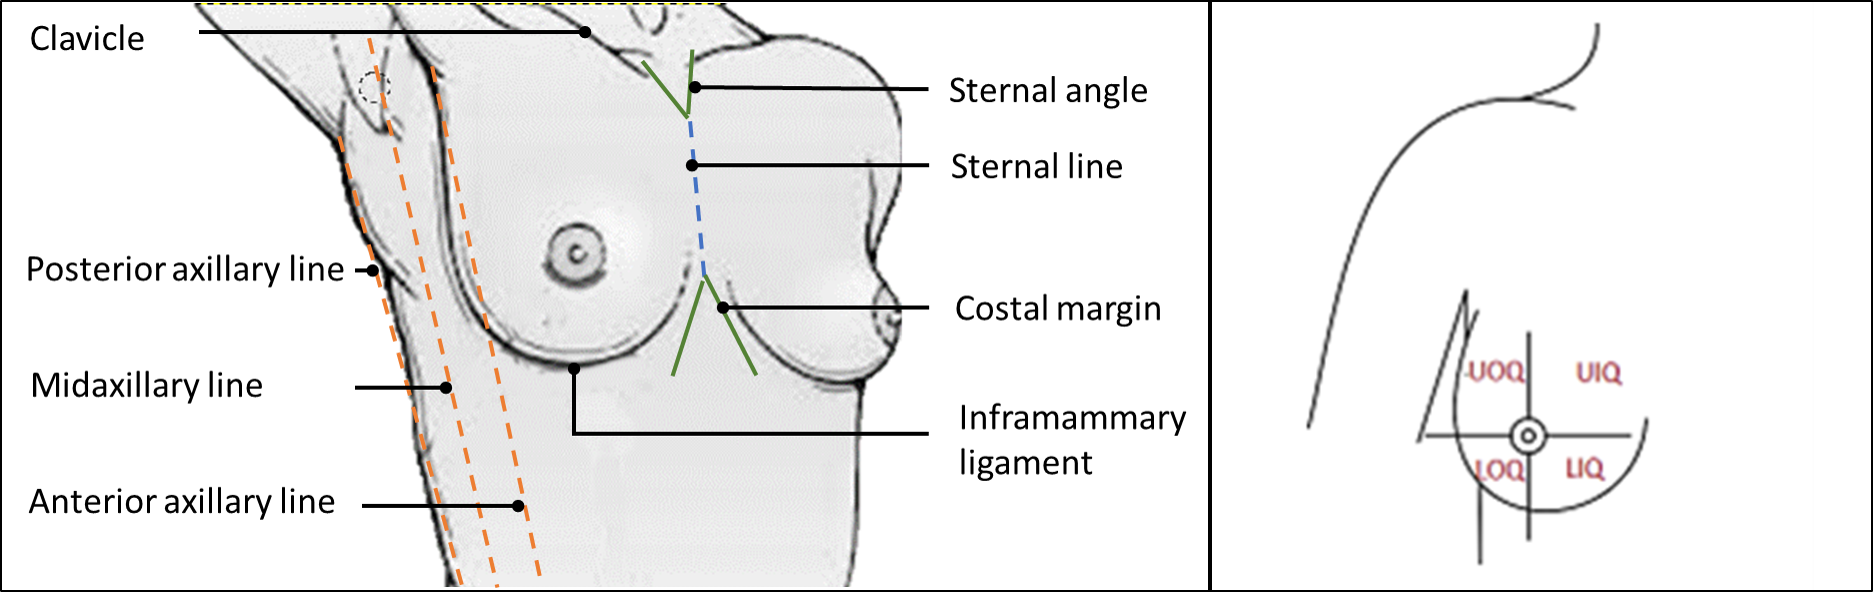
\includegraphics[width=\textwidth,keepaspectratio]{figures/Breast_quadrants_full.png}
  \caption{Left: thorax landmarks; Right: four breast quadrans \citep{vandeput2002considerations}}\label{fig:Breast_quadrants_full}
\end{figure}


 Anatomically, the adult breast is localized on top of the ribcage, between the clavicle superiorly and costal margin inferiorly. Its transverse boundaries are defined from the sternal line medially to the midaxillary line laterally (Figure\ref{fig:Breast_quadrants_full}). The intra-individual asymmetry (between left and right breasts) is considered as a normality for the young and the adult breast . The breast shape and contour are influenced by \citep{mugea2014aesthetic}:
 \begin{itemize}
 \item The volume of mammary gland in each breast quadrants.
 \item The amount of the subcutaneous and intra-lobular fat.
 \item The body contour of the chest wall.
 \item The muscular covering and thickness.
 \item The thickness and elasticity of the skin.
 \end{itemize}

Anthropomorphic characteristics of women breast were studied almost for the aim of cosmetic and reconstructive surgery.  \cite{vandeput2002considerations} measured distances between anatomical landmarks of the thorax of 973 women with aesthetically near-perfect breasts. The authors proposed different relations as guidelines to compute the recommended breast size parameters (nipple-mid clavicle distance, nipple inframammary fold distance) as a relation of body parameters (body height, torso width). In their study, a poor correlation was found between body height or weight and breast volume. Contrariwise a high correlation was found between the nipple to  inframammary fold distance or the nipple to mid clavicle distance and the thorax width. \cite{catanuto2008experimental} mentioned that the breast shape after surgery cannot be predicted by volumetric measurements only; they have proposed additional measures (areas, distances or angles) allowing unambiguous characterization of the breast shape. According to the authors, the curvature of the thoracic surface is the most relevant parameter to evaluate the outcome of a reconstructive breast surgery.


\subsection{Internal structures}\label{subsection:internalstructures}

Breast heterogeneous structure includes a mixture of parenchyma and adipose tissue (Figure\ref{fig:breastanatomy}). The breast parenchyma consists of glandular components, lymphatic network and blood vessels \citep{clemente2011anatomy}. Skin, Cooper's ligaments and fascias are the supporting system of the breast; their interconnection and intersections with the pectoral muscle fix and support the breast soft tissues \citep{mugea2014aesthetic}.

The \textbf{ adipose tissue} is the predominant tissue of the breast that fills up depressions between the deep and superficial fascia. In the intra-fascial space, adipose tissue surrounds and is dispersed among the glandular structures. Fat properties and its spatial distribution give the breast a soft consistency. The main aim of this tissue is to protect the lobes and lactiferous ducts.

The \textbf{ glandular tissue} is represented by breast lobes. A healthy female breast is made up of 12-20 lobes. They are distributed centrally and laterally within the breast. The total amount of glandular tissue depends on the hormonal fluctuation, age and physical state.  Mammary ducts arise from the lobes as branches and connect them to the female nipple. There are about 10 duct systems with a tree-like structure in each breast that carry the milk from the lobes to the nipple. The dark area of skin surrounding the nipple is called the areola. \cite{huang2011characterization} have studied the breast shape and fibro-glandular distribution using dedicated breast CT images. This study shows that the glandular tissues is situated in the central portion of the breast. In prone position about 60 $\%$ of glandular tissues is located near to the nipple. A mean percentage of glandular tissue was computed by \cite{yaffe2009myth}, the values varied from 13.7$\%$ to 25.6 $\%$ within different groups. They also mentioned a drop in glandular fraction with the advancing age. 


\begin{center}
\begin{figure}[h]
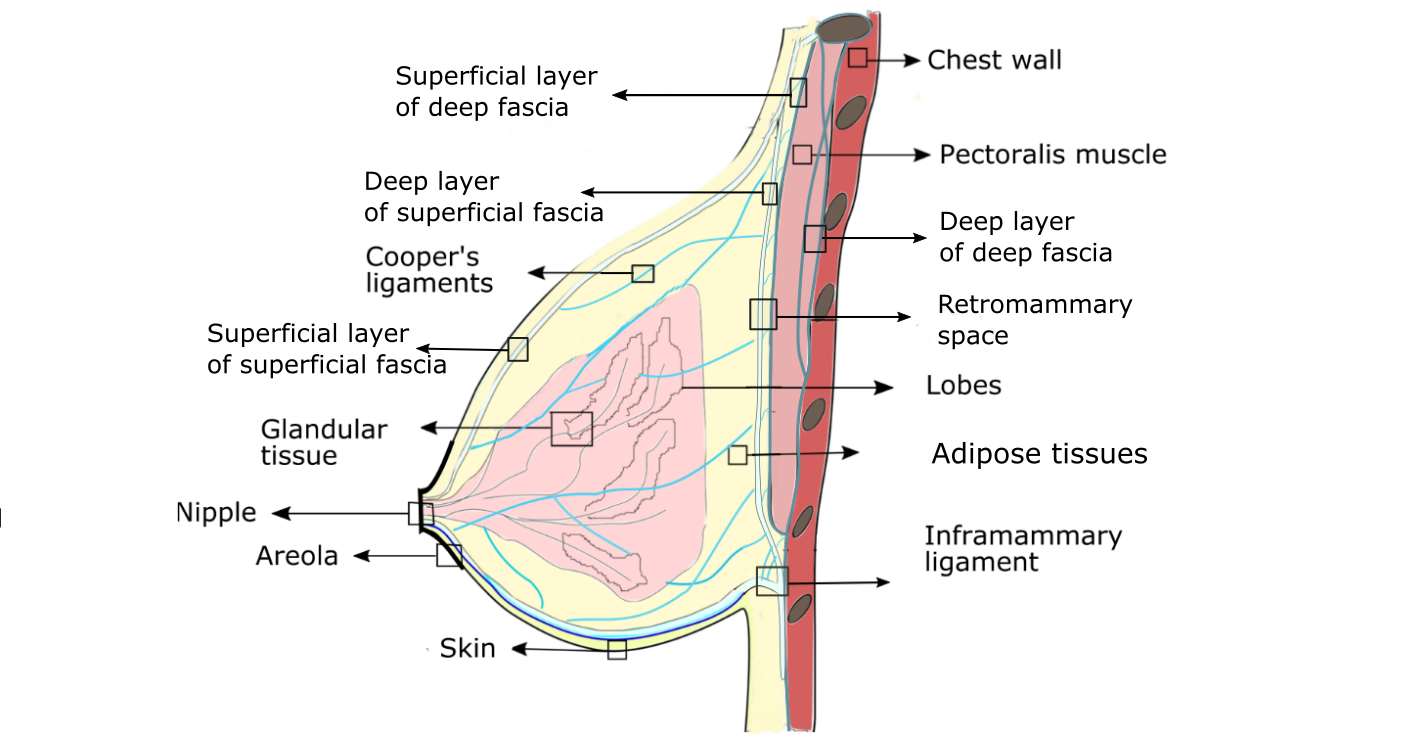
\includegraphics[width=\textwidth,keepaspectratio]{figures/anatomieSeinEuBlack2.png} 
\caption{Breast anatomy, \citep{clemente2011anatomy}}
\label{fig:breastanatomy}
\end{figure}
\end{center}

 A layer of adipose tissue and connective fascia separates the breast from the pectoral muscle forming a retro-mammary fat space.
 
The \textbf{skin} is the covering breast layer which provides protection and receives sensory stimuli from the external environment. It is a heterogeneous organ composed of 3 layers (see Figure \ref{fig:skinanatomy} , \citep{kanitakis2002anatomy} ): epidermis (dead cells) mainly composed of keratin, dermis composed of collagen and elastin fibers in a viscous matrix made of water and glycoproteins and hypodermis, mainly composed of adipocytes cells.


\begin{figure}[!h]
\centering
\centerline{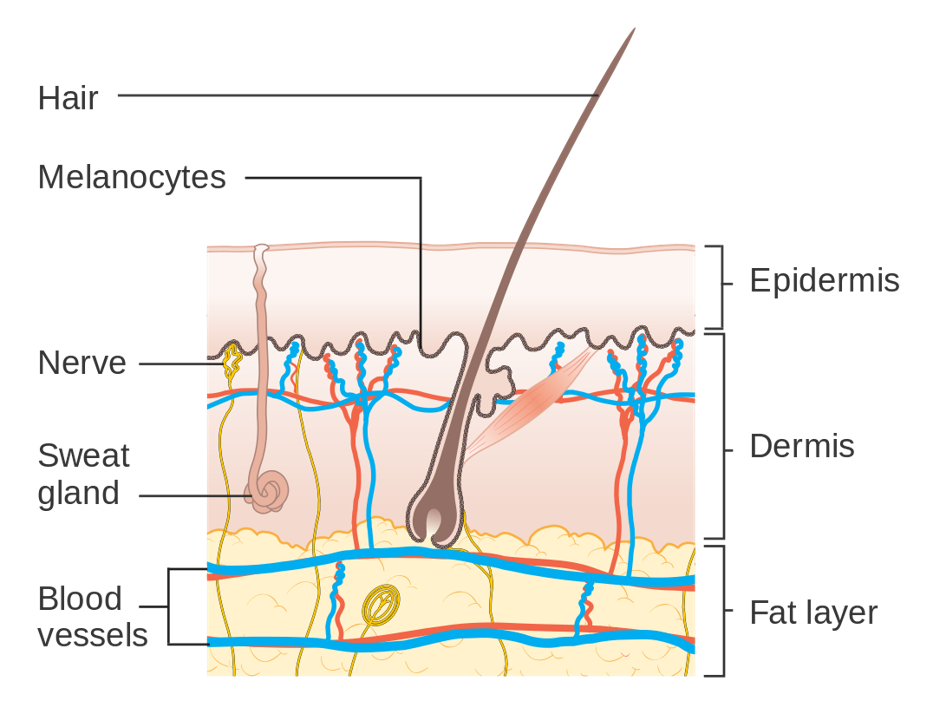
\includegraphics[width=0.5\textwidth,keepaspectratio]{figures/skin_2.jpg} }
\caption{Skin anatomy, \textit{Cancer Research UK}}
\label{fig:skinanatomy}
\end{figure}



The breast skin thickness vary from beast base to the nipple between $\sim$ 2 $mm$ and $\sim$ 0.5 $mm$. At the nipple areola region, the skin thickness measure 4-5 $mm$.
 \citep{andolina2011mammographic}. \cite{sutradhar_vivo_2013} studied the breast skin thickness of 16 different sectors radially oriented around the nipple. The thickness range proposed by the authors varies between $0.83 mm$ and $2.35 mm$ with a mean of $1.55 \pm 0.25 mm$. According to this study the skin thickness varies as follows: the lateral
region thickness is the thinnest among all the breast regions followed by superior/inferior and medial region; there is no significant difference between the inferior and superior breast regions; in the radially exterior region, the skin is thicker than in the radially interior region (close to the nipple).  \cite{ulger2003effect} found that, during the breast puberty, the breast volume increases and the skin thickness decreases in all regions.

The \textbf{connective tissue} is represented by Cooper's ligaments and fascial system. The breast fascial system is composed of deep fascia and superficial fascia. During puberty, breast is growing and the superficial fascia divides in two layers: the deep layer of the superficial fascia and the superficial layer of the superficial fascia \citep{kopans2007breast}.  Cooper's ligaments run throughout the breast tissue parenchyma from the deep layer of the superficial fascia beneath the breast to the superficial layer of superficial fascia where they are fixed (Figure \ref{fig:breastanatomy}). Because they are not taut, these ligaments allow the natural motion of the breast \citep{clemente2011anatomy}. Between the deep layer of the superficial fascia and the superficial layer of the deep fascia, a layer of connective loose tissue forms the retro-mammary space, allowing the breast tissue to slide over the chest \citep{mugea2014aesthetic}. In regions where the superficial fascia meets the deep fascia, suspension ligaments are created. One of these ligaments is situated at the level of the sixth and seventh ribs and is called the \textbf{inframammary ligament} \citep{bayati_inframammary_1995}. It evolves into the \textbf{deep lateral ligament} and the \textbf{deep cranial ligament} that are respectively attached to the axillary fascia and to the clavicle. The second meeting point of the 2 fascias is situated on the sternal line and is called the \textbf{deep medial ligament} (Figure \ref{fig:suspensoryligaments}). On the upper pole of the breast, near the second rib space, the deep fascia tightly connects with the 2 layers of the superficial fascia, here the third meeting point is created. The three ligaments are 3D structures, evolving from pectoral muscle toward the nipple underlying the skin surface.


The existence, the topography, and the thickness of the membranous layers of the superficial fascia have been studied in various regions of the body \citep{abu_membranous_2006}. According to the authors, the thickness of these superficial layers in both superior and inferior breast regions is equal to $88.12 \pm 7.70 \mu m$ and $140.27 \pm 11.03 \mu m$ respectively.

\begin{figure}[!h]
\centering
\centerline{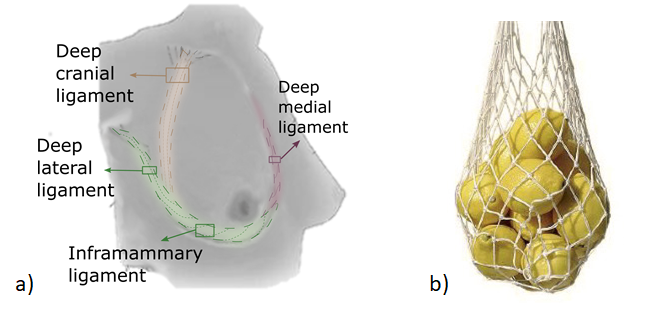
\includegraphics[width=0.7\textwidth,keepaspectratio]{figures/breastLigaments2.png} }
\caption{Suspensory ligaments. The suspensory ligaments together with the farcias constitute the breast sport matrix and ensure their inter-connection.   \citep{mugea2014aesthetic}}
\label{fig:suspensoryligaments}
\end{figure}


The lymphatic system is a vessel network which insures the transportation of white blood cells from tissues into the bloodstream. The majority of intramammary nodes are associated with the upper outer breast tissue and the lower outer part of the breast \citep{kopans2007breast}.  All intramammary lymph nodes are located in the lateral half of the breast along the margin of the breast parenchyma.  The lymphatic drainage of the breast extends from the subareolar plexus deep to and around the nipple (Figure\ref{fig:lyphaticDrainageandArtery} ).

The blood supply to the breast comes primarily from the internal mammary artery named successively subclavian, axillary, and brachial arteries (Figure\ref{fig:lyphaticDrainageandArtery}), from which lateral and internal thoracic arteries runs underneath the main breast tissue.

	
\begin{figure}[!h]
\centering
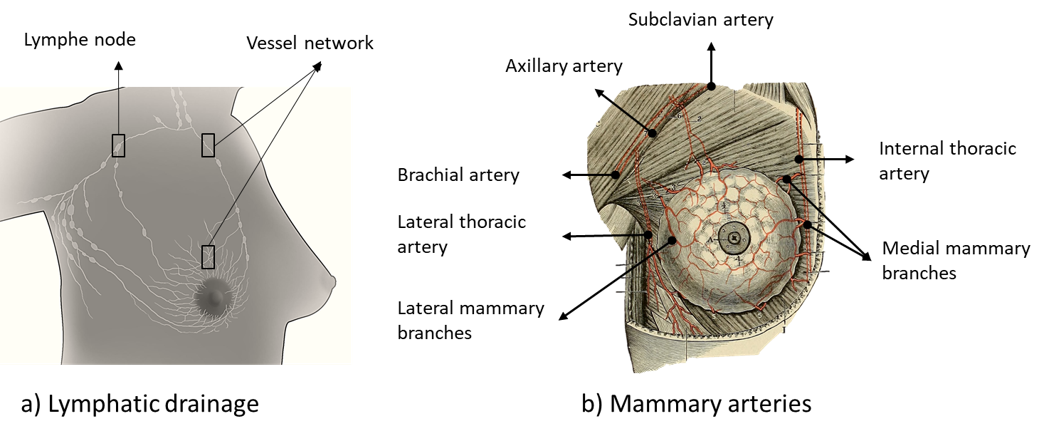
\includegraphics[width=\textwidth,keepaspectratio]{figures/lyphaticDrainageandArtery.PNG} 
\caption[Lymphatic system and Mammary Arteries for adult female breast. ]{Lymphatic system and Mammary Arteries for adult female breast.  Images reproduced from \cite{NCI_2012} and \cite{pilcher_breast_1917}}
\label{fig:lyphaticDrainageandArtery}
\end{figure}





\subsection{Adult breast texture changes}\label{subsection:adultbreasttexturechanges}

The female breast undergoes substantial changes during the woman's lifetime.  Most changes are caused by hormones and by woman's physiological condition. Important changes in female breast stiffness and composition occur during the menstrual cycle, pregnancy and menopause. 

There are 3 important changes during the menstrual cycle caused by hormonal changes \citep{andolina2011mammographic}. During the first phase, the estrogen (hormones) diffusion stimulates the epithelial cell multiplication and the enlargement of ductal structures. Next, during ovulation, epithelial cells begin to grow in the lobule due to progesterone hormone; an increase in blood flow is also noticed. In the last phase, the ductal structures and the lobes support an involution and a regression process. It must be mentioned that not all lobules regress, therefore during menstrual cycle new lobules can be created.   The work by \cite{lorenzen_menstrual-cycle_2003} showed that during the premenstrual phase the stiffness of fibro-glandular tissue and glandular tissue can change by 30\% and 14 \% respectively. They also have shown that in the middle of the menstrual cycle, the parenchyma volume increases of 38\% and the water content by 24.5\%.

During pregnancy, under the influence of estrogen and progesterone, the breast enlarges in volume and density, the veins dilate and the proportion of parenchyma tissues increases.  When lactation is weaned the breast returns to the pre-pregnancy state, and the atrophy of glandular, ductal, and stromal elements  is observed \citep{pandya_breast_2011}.

The menopausal breast contains a larger fraction of fatty tissues and reduce the number of ductal and lobular elements. During the first four years after menopause the breast is the subject of an atrophy process. The atrophy begins medially and posteriorly, then laterally, working its way to the nipple \citep{andolina2011mammographic}. In this period the breast loses progressively fat and stoma tissues, resulting in breast shrinkage and loss of contours.

 The breast support matrix can be stretched and attenuated by weight changes occurring during pregnancy and can relax with aging. These various changes can result in an excess of breast mobility over the chest and ptosis. 

\section{Breast Cancer}\label{section:breastcancer}

The first written description of breast cancer was on ancient Egyptian papyrus. At that time the treatment was considered futile and the woman was left without any medical assistance. Ancient Greeks, thought that the breast cancer was caused by an excess of black bile. It was thought that the monthly menstrual flow naturally relieved women of this excess, which explained why breast cancer was more common after menopause \citep{andolina2011mammographic}.

Nowadays, several researches \citep{pike_estrogens_1993,martin_webmd_2017} have shown that the cancer is always caused by damages to a cell's DNA. The initiation of the mutagenic process that may result in various genetic errors requires cell division.  A factor that increases cell proliferation will increase also the risk of cancer. The woman hormones, estrogen and progesterone, appear to impact the breast cell division rate \citep{ciocca_estrogen_1997,fanelli_estrogen_1996},  which explains the high rates of breast cancer in women ( $99\%$ of breast cancer occurs in women). The risks of developing a cancer is increased by various factors like age, genetics, family history or life style. According to \citep{martin_webmd_2017} the breast cancer risk factors can be explained by the exposure of women to the ovarian hormones during their lifetime.

The breast cancer is the second most frequent type of cancer and is the leading cause of death within women with cancer diagnosis \citep{spf_chiffres_2017}.  The Foundation for Medical Research \citep{frm_chiffres_2017} estimates the risk of developing breast cancer for french women as 1 in 8 with more than $47\%$ of cases diagnosed on women within 65 years old.
According to the French Public Health Agency \citep{spf_chiffres_2017} the incidence of breast cancer has increased by $138\% $ between $1980$ and $2005$. In United Kingdom and United States by year 2000 the death rate from breast cancer was reduced by almost 20\% and in 2005 was down by 25\% \citep{peto_uk_2000}. This significant improvement was attributable to the rise in the life expectancy and the upgrowth of screening technologies.


\subsection{Cancer classification }\label{subsection:breastcancerclasification}
Breast cancer type is determined by the specific cells that are affected. 
When a woman is developing a breast cancer, more frequently the primary tumor is developed in the epithelial cells, this type of tumor is called carcinomas. The primary tumor can also start in cells from other tissues such as muscle, fat or connective tissues. These types of tumors are called sarcomas, phyllodes, Paget disease and angiosarcomas but they are much rare \citep{acs_cancer_2017}. 

The carcinomas are then classified based on their location and how far the cancerous cell have spread. When the cancerous cells remain within the milk ducts or lobules, the cancer is classified as a non-invasive cancer. Otherwise, the malignant cancerous cells break through normal breast tissue barriers and spread out through other body organs, they are classified as invasive cancer \citep{andolina2011mammographic}. The most common types of carcinomas characterized by their location are: ductal carcinoma and lobular carcinoma. 

The invasive ductal carcinoma starts in the epithelial cells that line the milk ducts, whereas the invasive lobular carcinoma starts in the lobules. Both evolve through the surrounding tissues and may widespread to the other organs through bloodstream and lymph nodes (metastasize). 

Although the non-invasive carcinomas are not malignant, they have a 40\% chance to change to invasive carcinomas over a 30-year period. The non-invasive ductal carcinomas start and stay inside the milk duct. The non-invasive lobular carcinoma overgrowth the normal breast cells and stay inside the lobule. 

Invasive lobular carcinoma (ILC) \nomenclature{ILC}{Invasive lobular carcinoma} may be harder to detect on physical exam as well as imaging, like mammograms, than invasive ductal carcinoma. Moreover, compared to other kinds of invasive carcinomas, about 1 in 5 women with ILC might have cancer in both breasts.  Non-invasive ductal carcinoma is the more commonly detected form, making up 4\% of symptomatic cancers and 20\% of the cancer detected during a screening program. Its presence may be indicated on X-ray mammograms by microcalcifications \citep{acs_cancer_2017}.
 
\subsection{Breast cancer screening}\label{subsection:cancerscrenning}
Early detection remains the primary defense available to prevent the development of breast cancer. Early detection of breast cancer is made possible by  regular screening tests aimed to find suspicious legions before any symptoms can develop.  The principal benefit of the regular screening is the potential to prevent the premature and often prolonged, painful death of the individual. Studies have shown that regular mammographic screening resulted in a $63\%$ reduction in breast carcinoma death among women who actually underwent screening \citep{tabar_beyond_2001}. In 2012, the review of the UK screening program \citep{NHSBSP_2012} showed that it prevented 1300 deaths from breast cancer a year. 

Secondary benefits include a reduction in the trauma by treating earlier-stage lesions. Indeed, earlier found invasive carcinoma better respond  to treatment which means that the patient may avoid having a mastectomy or a chemotherapy.

Various worldwide countries have adopted organized breast cancer screening programs. Depending on the regional statistics and the estimated risk factors (age group, breast density, family history etc) the population is invited to participate to a free screening examination. In 1994, the French National Authority for Health approved a national screening program \citep{HAS_2016}. Since then, every woman within 50 and 74 years old, is invited one in two years for a clinical exam and a mammography.

The individuals who are suspected of having breast cancer, will have additional diagnostic tests as: diagnostic mammography, ultrasound (US)\nomenclature{US}{Ultrasound},Magnetic Resonance Imaging (MRI)\nomenclature{MRI}{Magnetic Resonance Imaging}, biopsy, blood test etc. The diagnostic test  not only helps to confirm or to infirm the screening result,but also, in case of positive test,  to determine the stage and the type of the breast cancer.
\section{Medical imaging}\label{section:medicalimaging}
 
Medical images are the techniques used in medicine to achieve information on human body internal structures or internal tissues properties. This information is then processed and analyzed in order to diagnose, monitor, or treat medical conditions. This technology encompasses different imaging modalities and processes, each with their own advantages and disadvantages. Next, the most relevant modalities for breast imaging are presented .

 

\subsection{X-ray mammography}\label{subsection:mammography}

X-ray mammography is a type of medical imaging that uses x-rays to capture images of the internal structures of the breast (FDA \nomenclature{FDA}{Food and Drug Administration } definition). In digital mammography (also known as Full Field Digital Mammography, FFDM\nomenclature{FFDM}{Full Field Digital Mammography}) x-rays are beamed through the breast to an image receptor (Figure\ref{fig:mammographyc ecam}). A detector converts X-rays to digital information. 

	
\begin{figure}[!h]
\centering
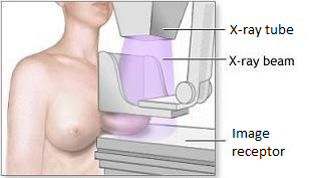
\includegraphics[width=0.5\textwidth,keepaspectratio]{figures/xraymammo.PNG} 
\caption[Mammographyc exam]{Mammographyc exam}
\label{fig:mammographyc ecam}
\end{figure} 

The mammography is used to detect parenchymal distortion, asymmetry, masses and clusters of microcalcifications within the breast.  These findings are not pathogenic
and require a tissue diagnosis to confirm the
presence of an invasive cancer, in situ cancer, or a nonmalignant finding. Microcalcifications ($\mu calc$\nomenclature{$\mu calc$}{microcalcifications}) are small calcium deposits embedded in a protein matrix .   They have x-ray attenuation coefficients substantially higher than breast tissue and therefore appear as bright spots in the x-ray images. The diameter of a microcalcification
is typically inferior to 1mm \citep{henrot_breast_2014}. In terms of form, breast microcalcifications can come in many shapes and sizes.  So, they can be round, linear, coarse or granular.  A mass is a radiological finding demonstrating an increased density versus the surrounding tissue. There is a large variation on mass size and shape, usually a suspicious mass is larger than 8mm and have irregular or speculated margins \citep{mckenna_abnormal_1994}.  Asymmetry and parenchymal distortion are visualised as tethering or indentation of breast tissue. They are the
third most common mammographic appearance of nonpalpable
breast cancer, representing nearly 6\% of abnormalities detected on screening mammography \citep{gaur_architectural_2013}. 

A standard mammographic protocol always includes breast compression prior to image acquisition. Women breast is compressed between two plates until a nearly uniform breast thickness is obtained. Nowadays, the European Commission recommends a force standardized breast compression, i.e. the compression stops at a level of force just below the subject’s pain threshold or to the maximum setting of the machine (not to exceed 200 N). Analog mammography used screen/film detector technology in order to display breast internal structures, thus a uniform breast compression was needed in order to ensure a uniform exposure over the breast volume. With digital mammography, the exposure variation could be corrected with post-processing, while the breast compression is still indispensable to hold the breast away from the chest wall, to reduce the blur due to physical motion, to reduce the absorbed dose of ionizing photons, to separate overlapping structures, to reduce image degrading scatter \citep{kopans2007breast}.


 
 %Breast cancer specialists estimate that breast cancer most frequently appears as microcalcifications and masses \citep{venkatesan_positive_2009}. 
Studies in different countries have assessed mammography sensitivity and specificity. The obtained sensitivities ranges between 81 and 88 \%, and the specificities between 83 and 98 \% \citep{kemp_comparing_2015,hofvind_sensitivity_2012}. The mammography sensitivity is mostly affected by dense breasts. A dense breast is a breast for which the  proportion of the fibroglandular tissues exceed greatly the proportion of fatty tissues. Fatty tissues are radiographically translucent, and lead to high intensity signal appearing on the mammographic images as dark areas. Meanwhile, the fibroglandular tissues and breast cancers tend to absorb more x-rays photons, therefore they will appear as white areas. The lack of contrast between the cancer and dense regions of the background will make the detection more difficult.      
 

\subsection{Ultrasounds}\label{subsection:ultrasound}

Breast ultrasound uses high-frequency sound waves to image breast tissues. The ultrasound technician put gel on the skin above the area of interest and moves the sound-emitting probe over the skin. The emitted waves are bounced by the breast soft tissues. The probe picks up the reflected waves and transforms them into a 2D image. 

For asymptomatic women, a careful investigation of lateral and profound breast tissues is needed to identify the suspicious lesions. The limited field of view of the ultrasound image prevents from seeing abnormalities that lie deeper in the breast. Consequently, the ultrasounds are not sufficient for regular screening and are used to complement other screening tests. However, it is widely used to investigate suspicious lesions found within mammography, clinical or self-examinations. Breast ultrasound is particularly effective in differentiating  cysts from solid lesions, but has a low sensitivity for breast which are the most common feature in addition to masses associated with breast cancer.
Breast ultrasound can also be used for differential diagnosis, local staging and intervention guidance.

Ultrasound elastography is a sonographic imaging technique combining the ultrasound technology with the basic physical principles of elastography. Elastography assesses tissue deformability by providing information on the tissue elasticity. It consists of either an image of strain in response to force or an image of estimated elastic moduli. This approach is somehow equivalent to clinical or self-examination, but with a higher precision.

Shear-wave elastography (SWE\nomenclature{SWE}{Shear-Wave Elastography}) uses focused pulses of ultrasound generated by the probe to induce soft tissues deformation. The tissues elasticity is assessed either by directly measuring soft tissues deformation or by measuring the speed of shear wave propagation. The combination of SWE with conventional ultrasound
increases the diagnostic performance for breast lesions, compared
with conventional ultrasound alone \citep{youk_shear_2017}.  Elastrography serves as a complementary tool to differentiate benign from malignant lesions by providing information about the lesion stiffness\citep{itoh_breast_2006,olgun_use_2014}
 
\subsection{Magnetic resonance imaging}\label{subsection:mri}

Magnetic resonance imaging (MRI) is a noninvasive procedure used in breast imaging for studying internal structure of the breast that cannot be properly imaged using standard x-ray imaging ( dense breasts).  It employs radio-frequency (RF\nomenclature{RF}{ Radio-Frequency waves}) waves and intense magnetic fields to excite hydrogen atoms. Body parts that contain hydrogen atoms (e.g. in water) are then imaged with contrasts depending on relaxation phenomenon characteristic of the tissues in the body. The quality of the image produced by MRI techniques depends, in part, on the strength of the received signal. For higher image quality, it is optimal to use an independent RF receiving coil placed in close proximity to the region of interest.  For breast imaging, dedicated breast MRI coils can be used. The patient is placed in prone position with the breast inside the coil and both arms by the sides of the body.

When the cancerous tumor develops, new vascularizations are created on the direct surrounding to provide oxygen.
Thus, for breast cancer imaging, a contrast agent may be used to enhance highly vascularized regions. These regions corresponding to the lesions are visualized due to their uptake of contrast agent. Contrast enhanced MRI is used as a screening modality for women with high risk of cancer.  

Low specificity and high cost of MRI restricts its use in a routine screening \citep{peters_meta_2008}. However, it is increasingly used for high-risk groups and for lesions that are difficult to detect with mammography or ultrasounds tests. 


\section{Conclusion}\label{section:conlusion}
Today, mammography the primary imaging modality used in breast cancer screening and plays an important role in cancer diagnosis. Ultrasounds and Magnetic Resonance Imaging are complementary imaging techniques used mostly for dense breasts and high-risk women.
 
In order to obtain an accurate reading, the mammography machine needs to compress the breasts.  The discomfort and pain produced by breast compression might deter women from attending breast screening by mammography  \citep{aro_psychosocial_1999,fleming_intermittent_2013}. In a study by \citep{dullum_rates_2000} more than 50\% of attendants (N= 1800) mentioned from moderate to extreme physical discomfort.  It has been reported that the
fear for pain itself can already be a reason to avoid getting the first mammogram \citep{andrews_pain_2001}, and that 15\% of those who skipped the second appointment cited as the main cause an unpleasant or painful first mammogram \citep{fleming_intermittent_2013,whelehan_effect_2013}.  Postpone the mammographic exam can lead to delayed breast cancer diagnoses and worse prognoses (expected outcomes) for some women.

The main direct cause of pain in mammography is the flattening of the breast which is directly linked to the applied compression force. Latest researches indicate that with a reduced level of compression (10N vs 30N), 24\% of women did not experience a difference in breast thickness. If breast thickness is not reduced when compression force is further applied, then discomfort increases with no benefit in image quality or average dose. Therefore, a detailed study on alternative breast compression techniques considering the patient comfort in addition to the image quality and ionizing radiation dose is needed.

The aim of this work is to provide a simulation framework capable to assess the patient physical comfort indicators, as well as the corresponding image quality and average glandular dose for breast compression with different paddles designs. The developed numerical methods would serve to build an optimal compression paddle in terms of latter listed parameters, and therefore increase the adherence to breast cancer screening. 

In this scope, a subject-specific biomechanical Finite Element (FE\nomenclature{FE}{Finite Element}) model is developed and evaluated on real deformations measured on MR images. The proposed model is then used to compute the tissues deformation associated to breast compression during mammography.  The resulting internal stress/strain intensities are then used as a first estimate of the physical comfort. The deformed breast geometry is the subject of a Monte-Carlo image simulation allowing to assess the image quality (IQ\nomenclature{IQ}{Image Quality}) and average glandular dose (\nomenclature{AGD}{Average Glandular Dose}AGD), in order to validate the image quality for the different strategies of compression we are considering.






\clearemptydoublepage
\part{Biomechanical breast modeling}\label{part:bioMecaModels}
\chapter{Background and state of the art}\label{chapter:bioMecaModelsBackground}


Finite elements models are widely used to estimate body parts deformation udder predefined boundary conditions. Several biomechanical models of the breast were recently developed providing physics-based predictions of tissue motion and internal stress and strain intensity.  In our work, we assume that the strain intensity obtained during the tissues deformation may by correlated with the patient discomfort. Thus, a biomechanical model obtained from the patient's MRI volume can be subsequently used to mimic breast compression during the mammographic acquisition. The resulting tissues strain cartography can be used as a first quantification of the patient inconfort.

This chapter provide theoretical background on continuous mechanic theory applied to soft tissues modeling. The principle of finite elements theory is defined including solid bodies and contact mechanics. A review of the existing biomechanical breast model is given describing the main challenges in the field and the proposed solution. These works proved the core foundation for the next developed patient specific breast model. 
      
\clearpage
\section{Continuous mechanics}
\label{section:continuousmechanics}
Continuum mechanics is a branch of mechanics that deals with the analysis of the kinematics and the mechanical behavior of materials modeled as a continuous mass. Continuum mechanics is based on the continuum hypothesis: the matter is continuously distributed throughout the space occupied by the matter. The basis for the hypothesis is how physical quantities, as for example pressure, temperature, and velocity, are measured macroscopically.

In this section the continuous mechanis theory applied to solids bodys was discribed using the following sources: \cite{belytschko_nonlinear_2013,abeyaratne_continuum_2012}.
\subsection{Deformation and strain}\label{subsection:defromationandstrain}
Continuous mechanics is the mathematical description of how physical objects that occur in nature respond to the application of forces.

	A \textbf{body} is the mathematical abstraction of an \textit{object} and is defined by its geometric and constitutive properties.  At a macroscopic level, a solid \textit{object} is described as homogeneous and continuous body, i.e. the substance of the object has a unique composition and completely fills the space it occupies thus, ignoring the granular (atomic) nature of matter. In continuous mechanics, a body $\mathcal{B}$\nomenclature{$\mathcal{B}$}{Body} is composed of a set of \textbf{particles} $p$ \nomenclature{$p$}{Particle or material point} (or material points). Each particle is located at some defined \textbf{point}  $x$ in three dimensional space. The set of all the points in space, corresponding to the locations of all the particles, is the \textbf{domain} $\Omega$ \nomenclature{$\Omega$}{Domain occupied by the body} occupied by the body in a given configuration, here also named $geometry$. A particular body can change its configuration and therefore the occupied region in the space when exposed to some external stimuli like force, pressure or heat.
	
 The \textbf{configuration} of a body is defined as a one-to-one mapping between the particle $p$ and position $x$, $\Omega_0 = \chi_0 (\mathcal{B})$ (see figure \ref{reference_config_theory}). To describe the solid's respond to external stimuli one needs to know the changes in geometrical characteristics between at least two configurations: the configuration that one wishes to analyze $\Omega_1$ \nomenclature{$\Omega_1$}{Current or analyzed body configuration }, and the \textbf{reference configuration} relative to which the changes are to be measured $\Omega_0$  \nomenclature{$\Omega_0$}{Reference body configuration }. Here, see figure \ref{reference_config_theory}, the mappings $\chi_0$ and $\chi_1$ take $p \rightarrow X$\nomenclature{$X$}{Point position on the reference configuration} and $p \rightarrow x$\nomenclature{$x$}{Point position on the current configuration}, thus $X$ and $x$ are the positions of particle $p$ in the two configurations under consideration.

Frequently, the reference configuration is fixed for a given study and is chosen arbitrary in a the most convenient way among all the configurations that the body can sustain. 
 
 The \textbf{deformation} of the body from the reference configuration $\Omega_0$ is characterized by the next defined mapping $\Phi$:
 \begin{equation} 
 x = \Phi(X) = \chi_1(\chi_0^{-1}(X)), \ \ \  where \ \  X \in \Omega_0 \ and \ x \in \Omega_1
 \label{referenceToCurrentCoordinates}
 \end{equation}
 
 The \textbf{displacement} $u$\nomenclature{$u$}{Particle displacement} of a particle is the difference between its position in the analyzed configuration (or current configuration) and its position in the reference configuration.
 \begin{equation}
 u(X) = \Phi(X) - X
 \end{equation}


\begin{figure}
\begin{center}
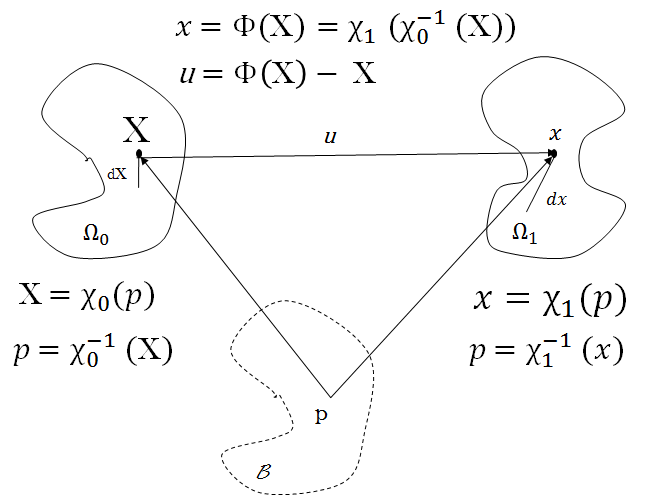
\includegraphics[width=0.7\textwidth,keepaspectratio]{figures/referenceFig.png} 
\caption{ The position of a particle in the reference and current body configurations.}
\label{reference_config_theory}
\end{center}
\end{figure}

Suppose that $G(\Omega_1)$ is the value of some extensive physical property  associated with the body $\mathcal{B}$ in the current configuration (such as the body mass $m$\nomenclature{$m$}{Body mass}). There exists a density $g(x)$ such that:
 $$G(\Omega_1) = \int_{\Omega_1} g(x)dv$$  
 where $dv$ is the volume of the material element.
 Thus, the property $G(\Omega_1)$ is related to the body while the density $g(x)$ is related to the position of the body particle.
\subsubsection*{Eulerian and Lagrangian formulations}
There are two classical techniques used to describe the body physical characteristics depending on the choice of independent variables.
 Some physical characteristics, such as mass density, can be defined for each individual particle. In such cases, the body characteristics are defined by the function $$m = \mathcal{M}(p)$$ for all $p \in \mathcal{B}$. Here the coordinate system remains consistent and moves with the particle. Therefore, the coordinates of both, the particle and the attached variable, do not change along the deformation. A particle is an abstract entity and cannot be used in numerical calculations, thus it is described by its location in reference configuration $p= \chi_0^{-1}(X)$ .
 $$m =  \mathcal{M}(p) = \mathcal{M}(\chi_0^{-1}(X))$$
 We call $X$ Lagrangian or material coordinates and their application is called Lagrangian or material description.  
 

Instead of defining body characteristics as a function of body particles, one can define it directly as a function of particle location in current configuration by using the relation $ x = \chi_1(p)$, and therefore 
$$m = \tilde{ \mathcal{M}}(x) = \mathcal{M}(\chi_1^{-1}(x))$$
 Here the coordinate system is fixed and the particles coordinate are changing. Therefore, the position of particle and any related quantity changes during the deformation.We call $x$ Eulerian or spatial coordinates and their application is called Eulerian or spatial description.
 
 These approaches are distinguished by three important aspects: the mesh description, the stress tensor and momentum equilibrium and the strain measure. The advantages and drawback of these two formulations will be discussed later in this chapter. Further, only Lagrangian formulation is used to describe the continuous deformation of soft tissues.       

\subsubsection*{Deformation gradient}\label{deformatiogradient}

In mathematical formulation the deformation gradient tensor $F$\nomenclature{$F$}{Deformation gradient} is the Jacobian matrix of the deformation $\Phi(X)$:
\begin{equation}
F = \frac{\partial \Phi (X)}{\partial X} = \frac{\partial x}{\partial X}
\end{equation}

Considering infinitesimal quantities, the deformation gradient relates the segment $dX$ in the reference configuration to the corresponding deformed segment $dx$ in the current configuration (Figure \ref{reference_config_theory}) 
\begin{equation}
dx = F \cdot dX.
\label{deformationGradRelation}
\end{equation}

In addition to the mapping of such vectors, the deformation gradient tensor allows also the mapping of differential volumes as:
\begin{equation}
dv = det(F)dV = JdV
\end{equation}

The Jacobian determinant of the deformation gradient tensor $J$\nomenclature{$J$}{Jacobian determinant of the deformation gradient tensor} is a measure of the volume variation during the deformation. It can be used to relate extensive physical properties in the current and reference configurations:
\begin{equation}
\int_{\Omega_1}g(x)dv = \int_{\Omega_0}g(\Phi(X))JdV
\label{JacobianRelation}
\end{equation}

\subsubsection*{Decomposition of the deformation gradient tensor into rotation and stretch}\label{deformationgradienttensor}
The deformation gradient tensor $F$ completely characterizes
the body deformation in the vicinity of a particle p. This deformation consists of a rigid body rotation and body \textit{stretch} (see Figure \ref{deformationGradientDecom}). As $dX$ and $dx$ are differential segments, the map $F$ is not affected by rigid-body translations.  

\begin{figure}
\begin{center}
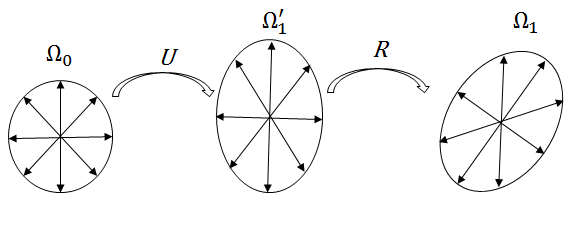
\includegraphics[width=0.7\textwidth,keepaspectratio]{figures/deformationTensorDecomposition.png} 
\caption[]{Decomposition by rotation and a stretch of a material particle.  }
\label{deformationGradientDecom}
\end{center}
\end{figure}


Generally, the body stretch is defined as the ratio of the deformed line elements to the length of the corresponding undeformed line element \nomenclature{$l$}{body stretch}
\begin{equation}
l = \frac{\vert dx \vert}{\vert dX \vert},
\end{equation} 
and consists locally on three mutually orthogonal stretches named \textbf{the principal stretches}.

According to the polar decomposition theorem, the deformation tensor can be written as the product of a proper orthogonal tensor $R$ representing the rotational part, and a symmetric positive defined tensor $U$ representing the body distorsion. 
\begin{equation}
F = R \cdot U.
\end{equation}
where $U$ and $R$ are given by the relations $U = (F^T \cdot F)^ {\frac{1}{2}} $ and $R = F \cdot U^{-1}$. The essential property of tensor $U$ is that it is symmetric and positive, therefor it has three real positive eigenvalues
$\lambda_1, \lambda_2, \lambda_3$ and a corresponding triplet of orthonormal eigenvectors $r_1, r_2, r_3$. Thus then an infinitesimal segment $dx$ is stretched by the tensor $U$, the segment is distorted in the principal direction of U by amounts of the corresponding eigenvalues of U. 

The tensor $U$ is also called the \textbf{right stretch tensor}.  Since there is a one-to-one relation between $U$ ans $U^2$, for the simplification of numerical calculus the stretch tensor can by replaced by the \textbf{Green deformation tensor} $C = F^T \cdot F$.



There are three particular functions of $C$ called the principal invaraints. 

\begin{equation}
\label{principal_invariants}
I_1(C) = tr C, \ \ I_2(C)=\frac{1}{2}\left[ trC^2 - \left(tr C \right)^2 \right], \ \ I_3(C)=det(C) .
\end{equation} 

These functions are related to the three principal stretches by the next relations:
\begin{equation}
\label{principalstrechinvariantsrelation}
I_1(C) = \lambda_1^2+\lambda_2^2+\lambda_3^2, \ \ I_2(C) = \lambda_1^2 \lambda_2^2 + \lambda_2^2 \lambda_3^2+ \lambda_3^2 \lambda_1^2, \ \ I_3(C) = \lambda_1^2 \lambda_2^2 \lambda_3^2
\end{equation}

The essential property of the principal invariants is that they don't change under coordinate transformations for a given body configuration. Their use to compute the body stretch will be an essential part of constitutive modeling, because the behavior of a material should not depend on the coordinate system.

It can be also shown that:
\begin{equation}
\label{eq:detinvariantrelation}
det(C-\mu I) = -\mu ^3+I_1(C)\mu ^2-I_2(C)\mu +I_3(C)
\end{equation}. 



\subsubsection*{Strain measures}\label{strainmeasure}
Referring to small deformations, the engineering nominal strain is defined as the ratio of the change in length of the deformed line element to the length of the corresponding undeformed line element:  
\begin{equation}
\epsilon = \frac{ dx  - dX }{	dX }
\end{equation}

When the body is not deformed, the deformation gradient $F$ and therefore the right stretch tensor $U$ is equal to identity tensor $I$. The strain in such a case is equal to zero. 

For most biological soft tissues, large deformation has to be considered. In that case, the previously defined strain is no more applicable. For large deformations, a measure of strain can be any monotonically increasing function related to stretch in a one-to-one manner, this function has to vanish in the reference configuration.

In orthogonal coordinate system, an admissible function is 

\begin{equation}
f(x) = \frac{1}{m}(x^m-1) \ for \ (m \neq 0)\  \ and \ ln(x) \ for \ (m=0)
\end{equation}


For $m = 0$ the function represents the Hencky strain tensor, 

\begin{equation}
E = ln(U), 
\end{equation}

for $m=1$  the function represents the Biot strain tensor 
\begin{equation}
E = U-I,
\end{equation}
and for $m=2$ the Green-Lagrangian stain tensor:
\begin{equation}
E = \frac{1}{2}(U^2-I) =  \frac{1}{2}(C-I)
\end{equation}

The Green-Lagrangian tensor is commonly used in practice as, by using the relation \ref{eq:detinvariantrelation}, it can be computed without prior knowledge of the eigenvectors of the Green deformation tensor C.
%Here only Green-Lagrangian strain is introduced. The Green-Lagrangian tensor $E$ is defined as:
%\begin{equation}
%dx^2 - dX^2 = 2dX \cdot E \cdot dX
%\label{GLRelation}
%\end{equation}
%
%From \ref{deformationGradRelation} equation, $dx^2$ is written as
%$$dx \cdot dx = (F \cdot dX)\cdot (F \cdot dX) = (F \cdot dX)^T \cdot (F \cdot dX) = dX^T \cdot F^T \cdot F \cdot dX = dX \cdot C \cdot dX,$$
%therefore the relation \ref{GLRelation} becomes 
%$$dX \cdot C \cdot dX - dX \cdot I \cdot dX = dX\cdot 2E \cdot dX$$
%Since the above relation must hold for all $dX$, one can deduce that:
%\begin{equation}
%E = \frac{1}{2} (C - I)
%\end{equation}

\subsection{Stress measures}%\label{subsection:stressmeasure}

\subsubsection*{Body and contact forces}\label{bodycontactforces}
Generally, forces are categorized as internal and external forces. An \textbf{external force } is a force caused by an external agent outside of the system, and contrariwise an \textbf{internal force} is a force exchanged by the particle in the system. The external forces, in turn, are categorized in \textbf{body forces} (acting at the distance) and \textbf{contact forces} (acting on the body surface). The relation between body forces per unit undeformed volume $\tilde{b}(X)$ (Lagrangian coordinates) and body forces per unit deformed volume $b(x)$ is given by the following relation:
\begin{equation}
\tilde{b} = \frac{dv}{dV} b = Jb.
\end{equation}

The contact forces can act on the external surface of the body or on a imaginary internal surface enclosing a volume element (Fig. \ref{internalcontactForceDefinition}). 
In general terms, the stress (or the \textbf{traction vector}) $t^n(x)$ is defined as contact force per unit area $da$ in the limit as $da \rightarrow 0$. Therefore $t^n(x)$ varies from point to point in intensity and orientation depending on the $da(n)$ orientation.  The stress vector projection on normal axis $n$ defines the \textbf{normal stress vector} and its projection on the tangential axis define the \textbf{shear stress vector}.


\begin{figure}
\begin{center}
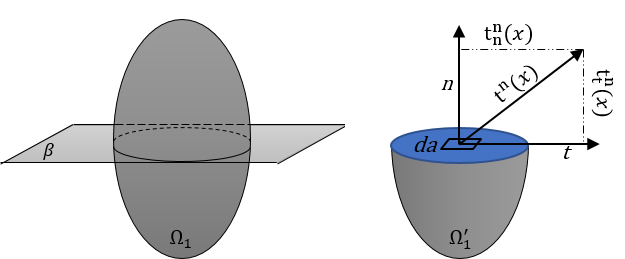
\includegraphics[width=0.7\textwidth,keepaspectratio]{figures/internalcontactForceDefinition.png} 
\caption[]{True stress vector $t^n(x)$ at point $x$ on the fictitious surface created  by the cutting plane $\beta$ of normal  $\overrightarrow n$ passing through the point $x$. }
\label{internalcontactForceDefinition}
\end{center}
\end{figure}

The stress on the boundary $\partial \Omega_1$ of the region occupied by the body is applied by external forces through physical contacts along the boundary. When formulating and solving a boundary-value problem, this stress defines the boundary conditions.


\subsubsection*{Cauchy's lemma}

Cauchy's lemma states that traction vectors acting on opposite sides of a surface are equal and opposite.
\begin{equation}
t^{-n}(x) = -t^n(x)
\label{chauchyLemma}
\end{equation}
\subsubsection*{Cauchy's Law}
Cauchy’s law states that there exists a Cauchy stress tensor $\sigma$ which maps linearly the normal to a surface to the stress vector acting on that surface, according to the next relation
\begin{equation}
t^n = \sigma \cdot n \ \ \ where \  \ t^n_i = \sigma_{i,j} n_j
\end{equation}

When large deformations are considered, the reference and current configurations of the body are significantly different and a clear distinction has to be made between them. The traction vector $t^n$ is defined in Eulerian coordinates (body current configuration) and is also called the \textbf{true stress}. Accordingly, the Cauchy stress tensor $\sigma$ is called the true stress tensor.

The definition of any measure with respect to the deformed configuration is less practical as it is usually unknown a priori. For the simplification of mathematical formulation, a new pseudostress is defined in the Lagrangian coordinate space named the \textbf{engineering stress}. The engineering stress has no physical meaning and has to be converted in to true stress for any interpretations.


\begin{figure}
\begin{center}
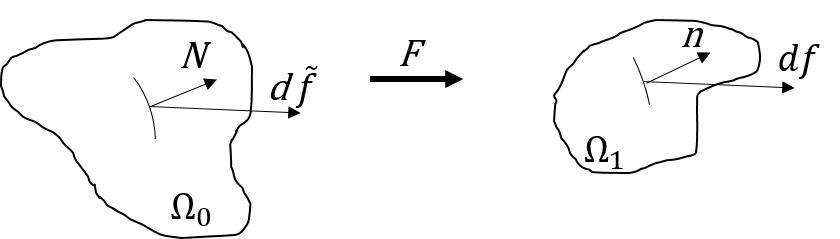
\includegraphics[width=0.7\textwidth,keepaspectratio]{figures/stressnotion.png} 
\caption[]{Deformation of area $dA$  into area $da$. The force $df$ acting on deformed area $da$ and the pseudoforce $d\tilde{f}$ acting on undeformed area $dA$}
\label{stressnotion}
\end{center}
\end{figure} 


Next, two pseodostress vectors are defined (Fig. \ref{stressnotion}):
\begin{itemize}
\item $T^N$ defined as the contact force $df$ per unit area $dA$ in reference configuration.
\item $\tilde{T}^N$ defined as the contact pseudoforce $d\tilde{f}$ per unit area $dA$ in reference configuration.  
\end{itemize}


Accordingly, two pseudostress tensors are defined based on pseudostress vectors:
\begin{itemize}
\item $T^N = P \cdot N$, $P$ is called \textbf{first Piola-Kircchoff stress tensor},
\item  $\tilde{T}^N = S \cdot N $, $S$ is called \textbf{second Piola-Kircchoff stress tensor}. 
\end{itemize} 
were $N$ is the normal vector of unit area $dA$.

The three stress tensors are linked by the next relation 
\begin{equation}
\sigma = J^{-1}F \cdot P = J^{-1} F \cdot S \cdot F^T
\label{PK12}
\end{equation}
\subsection{Conservation equations}\label{subsection:conservationequations}
Three conservation laws must be satisfied by physical system subject to any applied boundary conditions: \textbf{conservation of mass, conservation of linear momentum} and \textbf{conservation of angular momentum}. The resulting equations describe partially the mechanical behavior of a continuous body.

\subsubsection*{ Conservation of mass}
The mass $m$ of a body with the density $\rho$, that infills the space region $\Omega_1$ is given by :
\begin{equation}
m(\Omega) = \int_{\Omega} \rho(X)dV
\end{equation}
The mass conservation law requires that the body mass remains constant throughout all possible body configurations. For a Lagrangian formulation, this results in a relation between the body density in the reference configuration $\rho_1$ and the body density in the current configuration $\rho$.
$$\int_{\Omega_1} \rho_1 dv = \int_{\Omega_0} \rho_0 dV = const. $$

Using the relation \ref{JacobianRelation} one can deduce that:
\begin{equation}
\int_{\Omega_0} \left( \rho_1 J - \rho_0\right)dv = 0 \  \ and \  \ \rho_1 J = \rho_0
\end{equation}
\subsubsection*{Conservation of the linear momentum}

Assume that a body $\mathcal{B}$ is defined on a arbitrary region $\Omega_0$ with boundary $\Gamma_0$, and is subjected to a body-force $\rho_0  b$ and the surface traction $T^N$. And let $X$ be the particle location in the undeformed solid.
 The total force acting on the body $\mathcal{B}$ is defined as:
\begin{equation}
f = \int_{\Omega_1}\rho_0 b(X)dV + \int_{\Gamma_0} T^N(X)dA
\end{equation}
 
The conservation of the linear momentum requires that the total forces acting on the body to be equal to the time rate change of the linear momentum. In a static problem the time rate change of the linear momentum is neglected and thus an equilibrium equation is obtained.
\begin{equation}
\rho_0 b+\nabla_0 \cdot P  = 0
\end{equation}
Where the $P_{ji}$ are the components of first Piola-Kircchoff stress tensor
The equilibrium equation can be formulated in terms of the second Piola-Kircchoff stress tensor by using \ref{PK12} relations.
\subsubsection*{Conservation of angular momentum}
The conservation of angular momentum requires that the resultant momentum on any part of the body about a fixed point $\mathcal{O}$ equals the rate of increasing of its angular momentum (about $\mathcal{O}$). For a static problem, the integral form of the conservation of angular momentum is defined as:
\begin{equation}
\label{angularMomentum}
\int_{\Omega_0} X \times \rho_0 b(X)dV + \int_{\partial \Omega_0} X \times  T^N(X)dA = 0
\end{equation}

The relation \ref{angularMomentum} requires that the second Piola-Kircchoff stress tensor is a symmetric tensor:
\begin{equation}
S = S^T
\end{equation}
In summary, the conservation equations are fulfilled if and only if the following local conditions are fulfilled at each point in the body:
\begin{equation}
\rho_1 J = \rho_0, \ \ \nabla_0 \cdot S \cdot F^T + \rho_0 b =0, \ \ S=S^T 
\end{equation}
with the traction on the surface related to the stress through $\tilde{T^n} = S \cdot N$.
 For the simplification of mathematical calculus, the constitutive equations are formulated in terms of the second Piola-Kircchof stress tensor using the relations \ref{PK12}.

\subsection{Constitutive models}\label{subsection:constitutivemodels}
   The constitutive models, called also material models, define the relation between stress and strain of a physical system under the action of external stimuli. It is almost impossible to define a universal material behavior capable to model the material response to all possible conditions. Thus, for a given martial, several constitutive models can be defined depending on the studied characteristics. \\
	Biological materials are classified into:
	\begin{itemize}
\item \textit{ Isotropic or anisotropic materials:} in a isotropic (anisotropic) material the values of a property is constant (vary) with respect to the direction.

\item\textit{ Compressible or incompressible materials:} in a compressible (incompressible) material the volume changes (remains constant) during the deformation and the density remains constant. For a incompressible material the Jacobian determinant of the deformation tensor $J$ is equal to 1. 

\item \textit{Homogeneous or heterogeneous materials} in a homogeneous (heterogeneous) material the values of a property is constant (vary) with respect to the position within the body.
	\end{itemize}

Biological soft tissues are modeled using elastic materials model. The elasticity is the property of a solid material to return to its original size and shape when the influence of an external force is removed. In this case the strains are said to be reversible. 
	 
Considering small deformations, the stress-strain law of a linear material is given by the \textbf{Hook's law} $$\sigma = \lambda \epsilon,$$ where  the coefficient of proportionality $\lambda$ \nomenclature{$\lambda$}{Young's moduli} is named \textbf{Young's moduli}. 

 Elastic materials may be defined also with a non-linear stress-strain relationship. In such cases the elastic moduli ($\lambda $) is defined in function of strain $\epsilon$ $$\lambda = \frac{\partial \sigma}{\partial \epsilon} = f(\epsilon).$$

For example, for an elastic exponential material \citep{azar_methods_2002} the elastic moduli is computed using the function 
\begin{equation}
f(\epsilon) = b e^{m \epsilon},
\end{equation} 
where b and m are material parameters.
 
For large deformation the stress-strain relationship is deduced from a potential function. A \textbf{hyperelastic} material is an elastic material for which the work is independent of the deformation path. The material reversibility and path-independent behavior implies the absence of energy dissipation during the deformation. Thus there exist a \textbf{potential} function $W(E)$ such that $$S = \frac{\partial W(E)}{\partial E}= 2\frac{\partial \psi (C)}{\partial C}$$.\\
Moreover, if the material is isotropic, the stored strain energy $W$ of a hyperelastic material can by written as a function of principal invariants ($I_1, I_2, I_3$) of the Green deformation tensor $C$ previously defined in equation \ref{principal_invariants}.

We introduce below the most used potential functions for the characterization of biological soft tissues.
 
For the simplification of potential expressions, we define the first and the second deviatoric strain invariants:
\begin{center}
$\overline{I}_1=\frac{I_1}{I_3^{2/3}} $;  $\overline{I}_2=\frac{I_2}{I_3^{4/3}}$
\end{center}

We also define the \textbf{ Bulk moduli} \nomenclature{K}{Bulk moduli} as measure of a material's resistance to compression; the \textbf{shear moduli}\nomenclature{$\mu$}{shear moduli} as the ratio of shear stress to the shear strain; and the \textbf{Poisson ratio} \nomenclature{$\nu$}{Poisson ratio} as the ratio between longitudinal strain to the transverse strain describing the body shape change . For small deformation the Bulk moduli and shear moduli are linked to the Young's moduli and Poisson ratio by the next relations:
 \begin{equation} 
  K = \frac{\lambda}{3(1-2\nu)} \ \ and \ \ \mu = \frac{\lambda}{2(1+\nu)}
\end{equation}
  
\subsubsection*{Neo-Hookean potential function}
The Neo-Hookean \citep{treloar_elasticity_1943} law is an extension of the Hook's law to large deformations. The potential function is based only on the first invariant and is given by 
\begin{equation}
\label{eq:Neo-Hookmodel}
W =\frac{\mu}{2} (\overline{I}_1-3) + \frac{K}{2}(J-1)^2,
\end{equation}
where $\mu$ and $K$ are initial shear moduli and initial Bulk moduli respectively. 
\subsubsection*{Mooney-Rivlin potential function}
The potential function of a Mooney-Rivlin \citep{rivlin_large_1951} material is defined as:
\begin{equation}
\label{eq:mooneyRivlingmodel}
W=\frac{\mu_1}{2}(\overline{I}_1-3)+\frac{\mu_2}{2}(\overline{I}_2-3)+\frac{K}{2}(J-2)^2,
\end{equation}
where the constants $\mu_1$ and $\mu_2$ describing the material properties are linked to the initial shear moduli $\mu = (\mu_1+\mu_2)$. And the constant $K$ is the initial Bulk moduli. 

\subsubsection*{Gent potential function}
The potential function of a Gent \citep{gent_forms_1958} material model is defined as:
\begin{equation}
\label{gentmodel}
W=-\frac{\mu J_m}{2}ln\left(1-\frac{\overline{I}_1-3}{J_m}\right)+\frac{K}{2}\left(\frac{J^2-1}{2}-lnJ\right),
\end{equation}
 where $\mu$ and $K$ constants are the initial shear moduli and the initial Bulk moduli respectively. And $J_m$ is a parameter limiting the value of $(\overline{I}_1-3)$
\subsubsection*{Ogden model}
The Ogden \citep{ogden_large_1972} material model is based on the three principal stretches ($\lambda_1,\lambda_2,\lambda_3$) and $2N$ material constants, where $N$ is the number of polynomials that constitute the potential function:
\begin{equation}
\label{eq:ogdenmodel}
W= \sum^N_{i = 1} \frac{\mu_i}{\alpha_i}(\lambda_1^{\alpha_i}+\lambda_2^{\alpha_i}+\lambda_3^{\alpha_i}-3) + \sum_{k=1}^N \frac{K}{2}(J-1)^{2k},
\end{equation}
where $\mu_i$ and $\alpha_i$ are material constants, and $K$ is the Bulk moduli.

\subsubsection*{Yeoh model}
The potential function of Yeoh \citep{yeoh_characterization_1990} model is based on the first invariant:
\begin{equation}
\label{eq:yeohmodel}
W = \sum_{i=1}^N \mu_i(\overline{I}_1 - 3)^i + \sum_{k=1}^N \frac{K}{2}(J-1)^{2k},
\end{equation}
where the $\mu_i$ are material constants and $K$ is the Bulk moduli.

\subsubsection*{Govering equations of Lagrangian formulation} 
We consider a body $\mathcal{B}$ which occupies in the reference configuration the domain $\Omega_0$ with a boundary $\Gamma_0$`. The governing equations for the mechanical behavior of a continuous body are:
\begin{enumerate}
\item Conservation of mass $\rho_1 J = \rho_0$
\item Conservation of linear momentum $\nabla \cdot P + \rho b = 0$
\item Conservation of angular momentum $F \cdot P = P^T \cdot F^T$
\item Constitutive equations
\item Measure of strain $E = \frac{1}{2} (C-I)$
\item Boundary condition: $e_i \cdot N \cdot P = e_i \cdot \overline{t}$ on $\Gamma_0^{t_i}$
\item Internal continuity condition: $\llbracket e_i \cdot N \cdot P \rrbracket = 0$ on $\Gamma_0^{int}$
\end{enumerate} 

Where we note $\Gamma_0^{t_i}$ the set of prescribed traction  $\overline{t}$ on the body boundary $\Gamma_0$ ; and $\Gamma_0^{int}$ is the union of all surfaces where the stresses are discontinuous in the body (material interfaces).

The momentum equation together with the traction boundary condition and interior traction continuity condition are called generalized momentum balance (GMB) \nomenclature{GBM}{generalized momentum balance}.
\section{Finite Element Discretization}

\label{section:lagrangianmesh}
In continuous mechanics the body deformation is expressed in terms of partial differential equations (PDE \nomenclature{PDE}{partial differential equations}). For the majority of problems, the PDEs cannot be solved analytically, therefore approximation methods are developed. To this end, the finite element (FE) method has become the standard numerical calculation to compute such approximations. The computational domain, the unknown solution, and its partial derivatives are discretized, so as to obtain a set of algebraic equations for the function values at a finite number of discrete locations. The unknowns of the discrete problem are
associated with a computational mesh which represents a subdivision of the domain $\Omega_0$ into many small control volumes $\Omega_k$

\subsection{Eulerian and Lagrangian mesh description}

The mesh description depends on the chosen independent variables (Eulerian or Lagrangian formulation). An Eulerian mesh formulation is usually used to solve problems linked to fluid like materials and a Lagrangian mesh for solid like materials. In an Eulerian mesh, the Eulerian coordinates of nodes are fixed (coincident with spatial points) and the material point change in time (see Figure \ref{lagrangian_mesh}.b). In this case the mesh has to be large enough to contain the body in its current configuration. Throughout the deformation, the material points will belong to different elements. On the contrary, in a Lagrangian mesh, the Lagrangian coordinates of nodes are time invariant, nodal trajectory corresponds with material points trajectory and no material passes between elements (see Figure \ref{lagrangian_mesh}.a). 

\begin{figure}[!h]
\centering
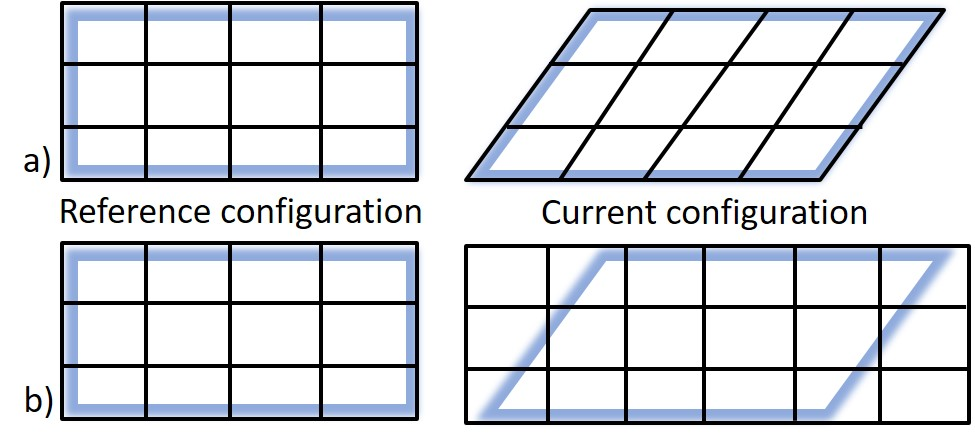
\includegraphics[width=0.8\textwidth,keepaspectratio]{figures/lagrangian_mesh.jpg} 
\caption{a) Lagrangian mesh formulation. b) Euler mesh formulation}
\label{lagrangian_mesh}
\end{figure}
 

In a Lagrangian mesh, the boundary and interface nodes remain coincident with body boundaries and material interfaces throughout the entire deformation. Thus, the boundary conditions are defined directly on the respective nodes. On the other hand, in a Eulerian mesh the boundary and interface conditions have to be defined on point which are not nodes. This implies important complications in multi-dimensional problems.  

An important drawback of a Lagrangian mesh affect mainly the large deformation domain. As the nodes are coincident with the material points, the elements deform with materials. Therefore, the magnitude of deformation is limited because of element distortion. The limited distortion that most elements can sustain without performance degradation or failure is a important factor in nonlinear analysis with Lagrangian formulation. 
 

\subsection{Lagrangian mesh}\label{subsection:lagrangianmesh}

The general approach of the FE method in Lagrangian formulation is shown in Fig. \ref{fe_method}. First the momentum equations with given boundary conditions are multiplied by a set of appropriate test functions. The test functions have to satisfy all displacement boundary conditions and to be smooth enough so that all derivatives in momentum equations are well defined. Then performing an integration by parts, the week formulation of GMB is obtained, also called the principle of virtual work \citep{belytschko_nonlinear_2013}. 

\begin{figure}[!h]
\centering
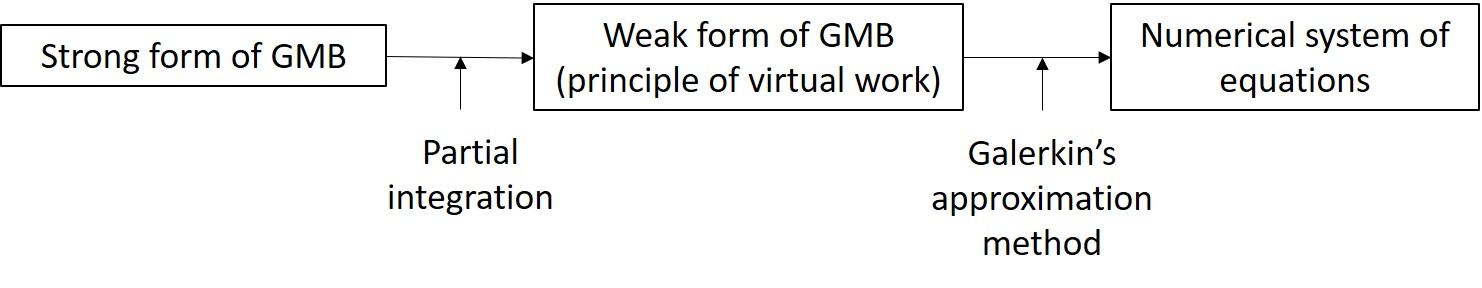
\includegraphics[width=0.8\textwidth,keepaspectratio]{figures/fe_method.jpg}
\caption{From strong formulation of the generalized momentum balance (GMB) to numerical equations.}
\label{fe_method}
\end{figure}




 The momentum equations and the traction boundary conditions, usually called the strong form, cannot be directly discretized by FE method. The strong formulation of the GMB equations impose the $C_1$ continuity conditions on the field variables. Therefore, the solution of this problem does not always exist. This is true especially in the case of complex domains with different material interfaces. In order to overcome these difficulties, weak formulations are preferred. The week formulation of GMB reduces the continuity requirements thereby allowing the use of easy-to-construct and implement polynomials. Because of the reduction in the requirements of function smoothness, the weak forms never give an exact solution but one can obtain a relatively accurate solution with the discretization refinement.



From the week form of the GMB equations, the numerical system of equations is formulated by using finite elements interpolants for the mechanical displacement and the test functions.   The whole domain is discretization into a number of smaller areas or volumes which are called \textbf{finite elements} and their assembly is called a\textbf{ mesh}. Elements can be of various shapes (as shown in Figure \ref{discretization}.b),  quadrilateral or triangular in two dimensions, and tetrahedral or hexahedron in three-dimensions.


\begin{figure}[!h]
\centering
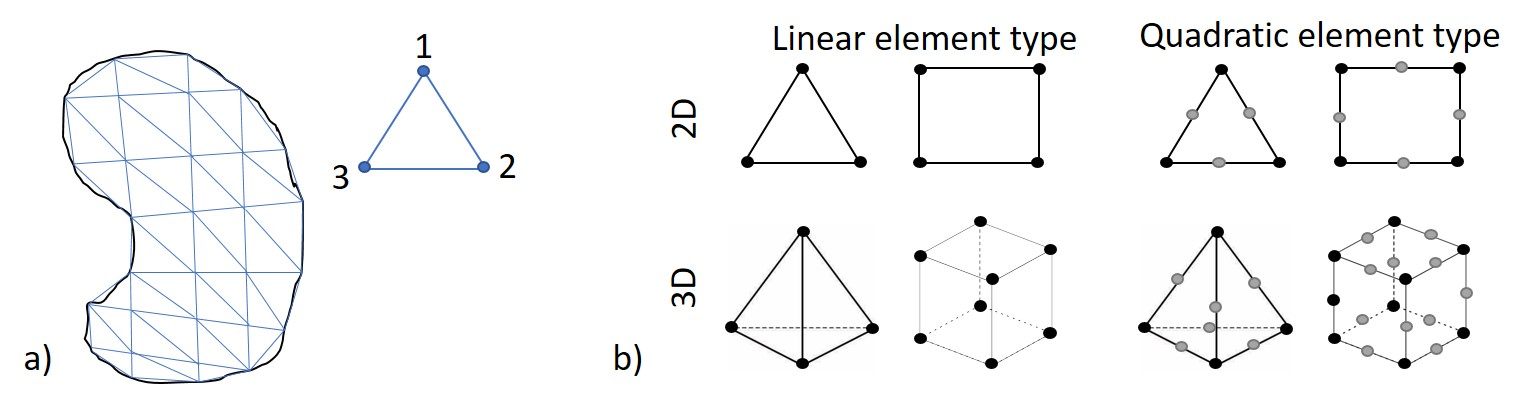
\includegraphics[width=1\textwidth,keepaspectratio]{figures/discretization.jpg} 
\caption{a) Discretization of  a 2D domain with triangular finite elements :Lagrangian mesh . b) Different types of finite elements}
\label{discretization}
\end{figure}

 The mechanical displacement is approximated at the discretization points called finite element\textbf{nodes}. The nodes are at the vertices corners of the elements for a linear type, and at the vertices corners and midsides of the elements edges for a quadratic type (figure \ref{discretization}.b). The displacement of each point within an element is interpolated from the values of the displacements of the nodes of the element. In this way, the problem of finding the displacement of every point within the body is replaced by the problem of finding the displacements of a finite number of nodes.
 
 As in a Lagrangian mesh the nodes are following the motions, for large deformation the finite elements can be highly distorted. Therefore, the elements shape quality is generally checked all along the deformation process. Several shape parameters for each element type have been proposed such as: aspect ratio, maximum corner angle, Jacobian ratio, skewness, parallel deviation, warping factor. The acceptable limit values of these shape factors are proper to the elements types. 
 
In the following, only the shape parameters of the linear triangular elements are presented \citep{ansys_theory_2017}.  
 \subsubsection*{Triangle aspect ratio }
 The element's shape aspect ratio is computed using only the vertices corner nodes of the element (Figure \ref{fig:aspectratio}). First, two lines are created: one through a node ($K$) and the midpoint of the opposite edge ($ K'$), the second through the midpoint of the others two edges ($J'$ and $ I'$). Then two rectangles are created, each rectangle have a pair of edges parallel to one of previously defined lines. The rectangle edges have to pass through the nodes and the triangle's edges midpoints. This construction is repeated for each triangle's node resulting in 6 rectangles. The aspect ratio of a rectangle is defined as the ratio between the longer and shorter side. Thus, the triangle's aspect ratio is defined as the maximal aspect ratio over the 6 rectangles divided by squared root of 3. 
 
 The best possible aspect ratio is 1 and is represented by an equilateral triangle. An element with an aspect ratio larger than 20 is considered as bad aspect element, large aspect ratio may degrade solution performance.
 
 \begin{figure}[!h]
\centering
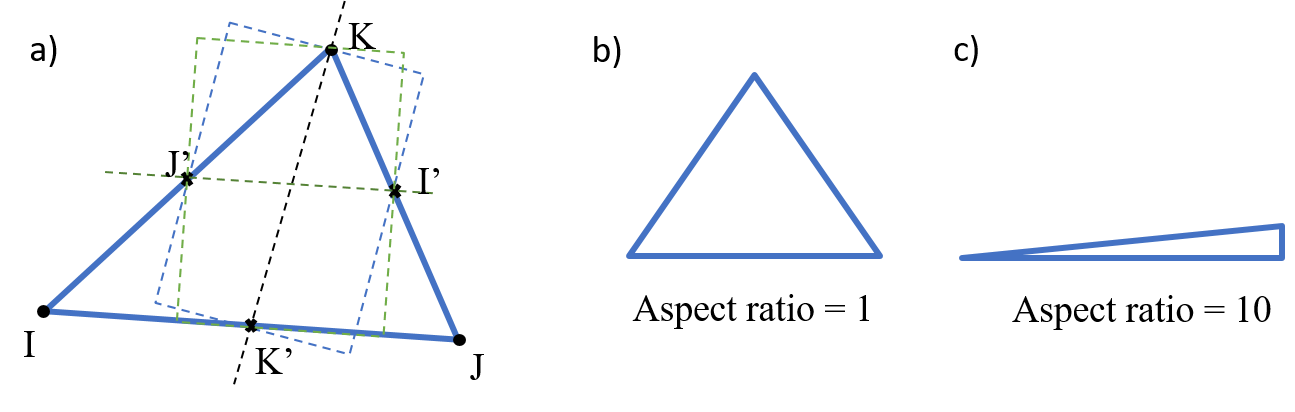
\includegraphics[width=0.9\textwidth,keepaspectratio]{figures/aspectRatio.png} 
\caption{Computation of the aspect ratio for a triangle}
\label{fig:aspectratio}
\end{figure}  

\subsubsection*{Triangle maximum corner angle}
The maximum corner angle is computed using nodes position in 3D space. The best possible maximum corner angle is 60\textdegree. An element having a maximal corner angle larger than 165\textdegree is considered as bad shape element, large corner angles may degrade the solution performance. Figure \ref{fig:cornerangle} shows a triangle with a good ( 60\textdegree) and bad ( 165\textdegree) quality. 

 \begin{figure}[!h]
\centering
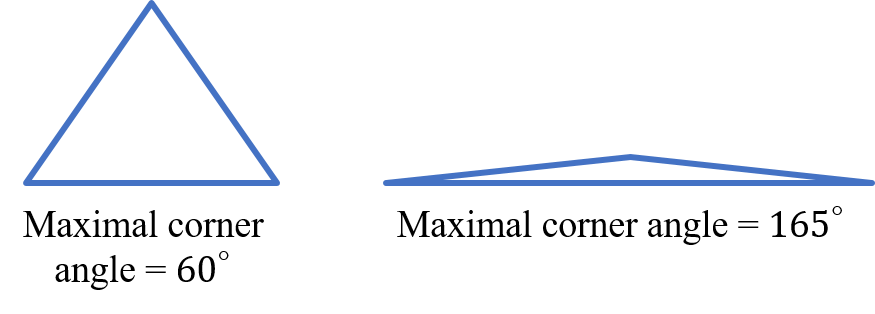
\includegraphics[width=0.6\textwidth,keepaspectratio]{figures/maximalcornerangle.png} 
\caption{Example of triangles with different maximal corner angles.}
\label{fig:cornerangle}
\end{figure} 

The aspect ratio and the maximal corner deviation of a tetrahedra is computed using the definition of the same measure on a triangle. The elements shape parameter is assigned as the worst value over the triangles defined by the tetrahedra's faces and cross-sections.  

\subsubsection*{Skewness }
The skewness of a triangular element is computed using the equivalent volume deviation method. It is defined as the difference between the optimal and real cell size over the optimal cell size. The optimal size is the size of an equilateral cell with the same circum radius. According to its definition, the value of 0 indicates an ideal cell, from 0 to 0.75 the cell is considered to have a good quality, from 0.75 to 1 the cell is considered to have a bad quality and a value of 1 indicates a completely degenerated cell (Figure \ref{fig:skewness}).   

 \begin{figure}[!h]
\centering
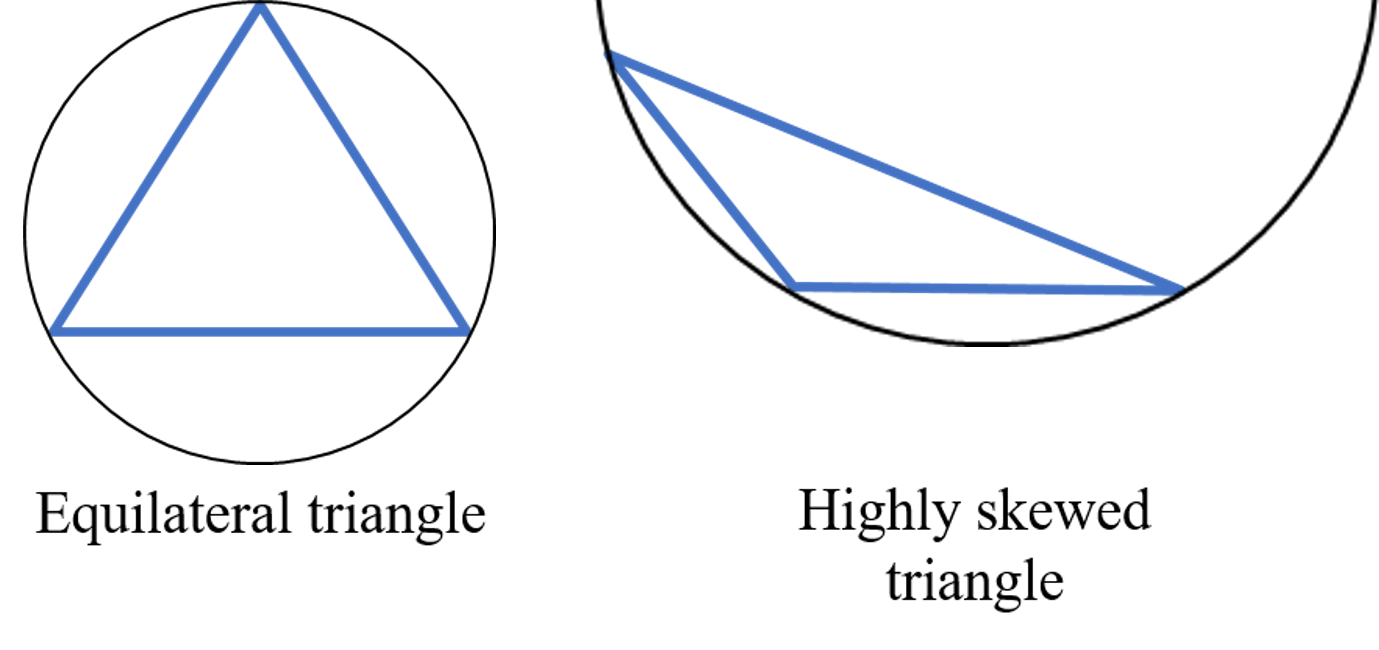
\includegraphics[width=0.6\textwidth,keepaspectratio]{figures/skewness.png} 
\caption{Example of triangles with different skewness with the corresponding circum radius.}
\label{fig:skewness}
\end{figure}
 
\section{Contact mechanics}\label{section:contactmechanics}

In order to transfer the loads between elements, the nodes have to be connected together. If two bodies are separated with no common nodes, no interaction will occur during the deformation and the bodies will pass through each other. Here, an asymmetric surface-to-surface contact method is used to solve the multi-body interaction problems.

Let's consider two different bodies $\mathcal{A}$ and $\mathcal{B}$ and their occupied domains $\Omega_A$ and $\Omega_B$ with boundaries $\Gamma_A$ and $\Gamma_B$ respectively (see Figure \ref{contact_bodies}). Also, we note $\Omega$ the domain of intersection of two bodies. The contact interface is the intersection of the surfaces of the two bodies:
$$\Gamma = \Gamma_A \cap \Gamma_B.$$
The intersection consists of two surfaces, usually distinguished as \textbf{target} and \textbf{contact} surfaces. For an asymmetric contact each surface has a single designation and the choice of the surfaces type is made following these next guidelines (the target surface property are enumerated in their priority order):
\begin{itemize}
\item if the body $\mathcal{A}$ is stiffer than the body $\mathcal{B}$, the surface $\Gamma_A$ defines the target and $\Gamma_B$ the contact surface;
\item if $\Gamma_A$ is a concave surface getting in contact with the convex surface $\Gamma_B$, the surface $\Gamma_A$ defines the target and $\Gamma_B$ the contact surface.
\item if the surface $\Gamma_A$ is larger than $\Gamma_B$, the surface $\Gamma_A$ denotes the target and the $\Gamma_B$ the contact surfaces.
\end{itemize} 
For the following, we identify $\Gamma_A$ as the target surface and $\Gamma_B$ as the contact surface (Figure \ref{contact_bodies}). 

 Sometimes, the asymmetric contact does not perform satisfactory results and a symmetric contact is needed. When defining a symmetric contact each surface coming in contact is designated to be both, contact and target surface type. Therefore, two set of contact pairs are defined. The symmetric contact may be used then the distinction between the contact and the target surfaces is not clear or to reduce the contact penetration, however it usually results in a more time-consuming solution.



\subsection{Contact inteface equations}%\label{governingequations}
 In the case of multi-body interaction, in addition to the standard mechanical governing equations, two more contact conditions have to be fulfilled: the two bodies cannot interpenetrate and the traction must satisfy momentum conservation on the contact interfaces.
   

 \begin{center}
\begin{figure}
\centerline{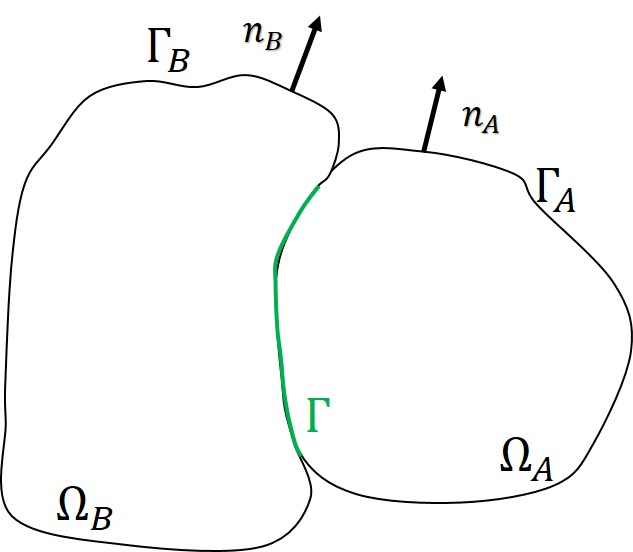
\includegraphics[width=0.4\textwidth,keepaspectratio]{figures/contact_bodies.jpg} }
\caption{Multi-body contact problem.}
\label{contact_bodies}
\end{figure}
\end{center} 
   
  \subsubsection*{Traction conditions}
  Traction conditions must follow the balance of momentum across the contact interface:
  \begin{equation}
  t_A + t_B=0
\end{equation}
On the contact boundary surface $\Gamma$ the traction vector is decomposed into its normal and tangential components:

$$t_A^n = t_A \cdot n_A,  \ \ \ t_B^n = t_B \cdot n_B$$
$$t_A^t = t_A - t_A^n n_A, \ \ \ t_B^t = t_B - t_B^n n_B$$

Therefore the momentum balance requires:
\begin{equation} 
t_A^n + t_B^n = 0, \ \ \ t_A^t + t_B^t = 0
\end{equation} 

 \subsubsection*{Inter-penetrability condition}
The bodies implied in a multi-body problem must fulfill the inter-penetrability condition:
\begin{equation}
\Omega_A \cap \Omega_B = 0
\end{equation}
Decomposing the displacement $u$ into its normal and tangential components $u^n$ and $u^t$ respectively the inter-penetrability condition can be written as:
\begin{equation}
t^n \leq 0, \ \ u^n-g n_a \leq 0, \ \ t^n(u^n-g n_a) = 0
\end{equation}
 Where $g$ is the gap between the two bodies and $n_a$ is the normal to the target surface.

\subsection{Surface interaction models}%

\label{subsection:surfaceinteractionmodels}
When two solid bodies are placed together under a nonzero normal force and acted upon by another with a tangential force, a \textbf{friction force} $f_{friction}$ tangential to the interface and opposite to the applied force is created. Depending on whether the applied force can overcome the friction force opposing it, the bodies may or may not move relative to each other. The body motion along the interface is called \textbf{sliding}. The \textbf{sliding force}, $f_{sliding}$ is the applied tangential force which causes the sliding motion between the two bodies.
  
Determining whether relative motion will or will not occur requires balancing the involved forces. According to the allowed relative body motion in tangential or normal directions, five types of surface interaction models are distinguished: bonded, rough, no-separation, frictional and frictionless. Table \ref{contactB} resumes each corresponding mechanical behavior. If the body motion is not allowed in normal or tangential direction, once the bodies get in contact, the respective components of traction are equals ($t_A=t_B$), which means that, for a pure \textbf{bonded} contact, the two bodies are considered as a unique solid body.    

\begin{table}[H]

\begin{center}
\begin{tabular}{||c|c|c||}
\hline
Name & body motion in normal direction & body motion in tangential direction \\
\hline\hline
Bonded & No & No\\
\hline
Rough & Yes & No, $f_{friction} \gg f_{sliding}$ \\
\hline
No-separation & No & Yes, $f_{friction} = 0$ \\
\hline
Frictionless & Yes & Yes, $f_{friction} = 0$ \\
\hline
Frictional & Yes & Yes, if $f_{sliding} > f_{friction}$\\
\hline
\end{tabular}
\caption{Surface interaction models and corresponding mechanical behaviors}
\label{contactB}
\end{center}
\end{table}

The \textit{frictional} contact behavior is defined using Coulomb friction law. For a continuous body the Coulomb friction model is applied at each point of the contact interface.
Considering that bodies $\mathcal{A}$ and $\mathcal{B}$ which are in contact within the surface $\Gamma$, then for all $x \in \Gamma$:
\begin{equation}
\label{stiking}
if \ \Vert t^t(x) \Vert < -\mu_f t^n(x),\ \ \Delta u^t=0 
\end{equation}
\begin{equation}
\label{sliding}
if \ \Vert t^t(x) \Vert = -\mu_f t^n(x),\ \ \Delta u^t=-k(x)t^t(x),\ \ k(x)>0
\end{equation}

Where $\mu_f$ is the material property named \textbf{friction coefficient},  $\Delta u^t$ is the slip incremental in the tangential direction and $k(x)$ is a variable computed from the momentum equation. The condition \ref{stiking} is known as the sticking condition: the tangential traction is less than the critical value, thus no sliding occurs. Reciprocally, condition \ref{sliding} is called the sliding condition.

When a frictionless contact model is used, $\mu_f = 0$, the tangential tractions vanish completely: $t_A^t = t_B^t = 0$. On the contrary, when a rough contact is modeled, the friction coefficient $\mu_f$ is equal to infinity, so that the sticking condition is always fulfilled. 

In practice, several contact models can be combined to model a physical contact between two bodies.   

\subsection{Contact formulation algorithm: Pure Penalty model}%\label{subsection:purepenalty}

\subsubsection*{Pinball region}

Contact formulation presents two primary difficulties from a computational point of view. First, the traction conditions have to be estimated for each considered frictional model. And second is the unpredictability of regions which will get in contact with each other during the deformation process.

The region of contact depends on materials properties and imposed boundary conditions; therefore, it is difficult to know a priori where the surfaces will be in contact. To formulate analytic equations, one has to know exactly the nodes involved in the contact process. Therefore, during body deformation, the program calculates if the contact is \textit{opened} or \textit{closed}. The status is defined using a sliding pinball (Figure \ref{fig:pinball}). The pinball slides over the contact surface nodes and searches for the target surface. If the node to surface distance is smaller than the pinball radius, the contact is considered to be closed (Figure \ref{fig:pinball}, green nodes) otherwise the contact is considered to be opened (Figure \ref{fig:pinball}, gray nodes).    

\begin{figure}[!h]
\centering
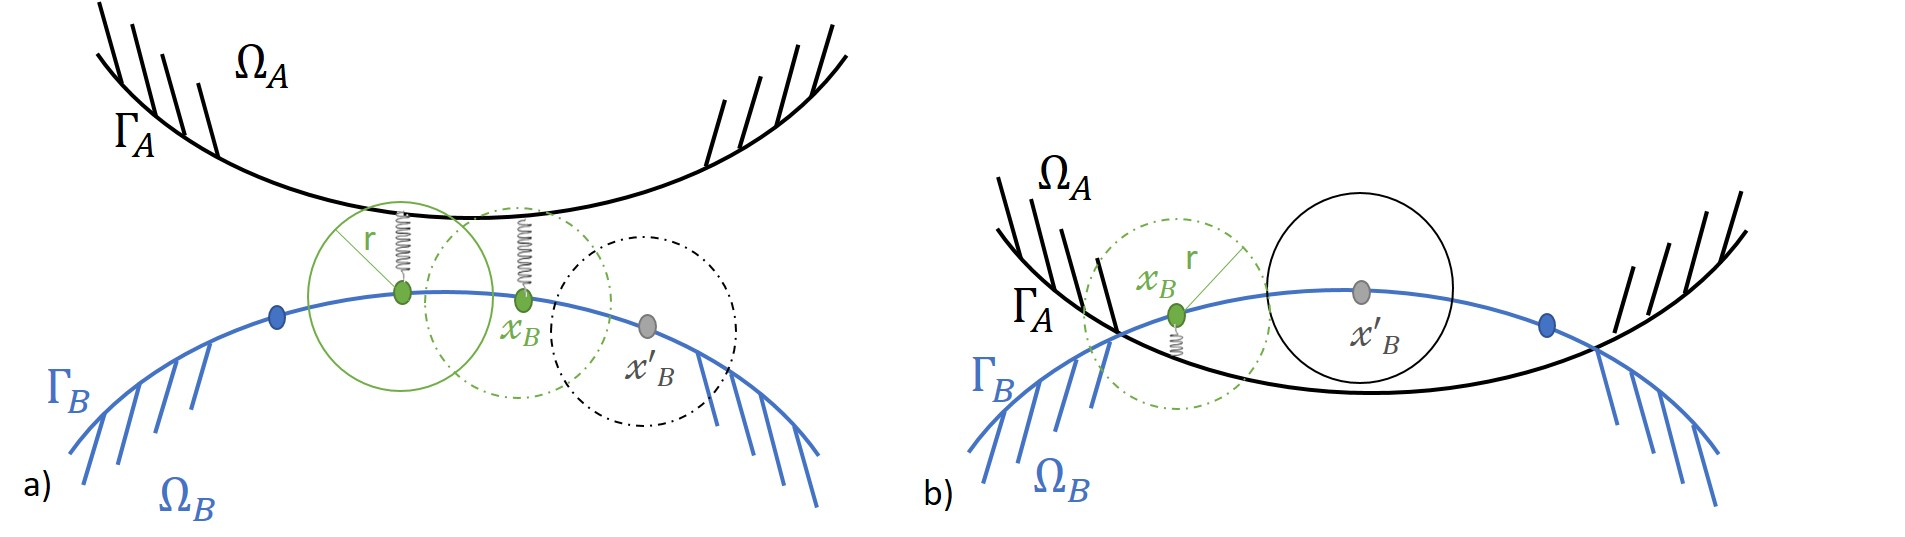
\includegraphics[width=1\textwidth,keepaspectratio]{figures/pinball.jpg} 
\caption{Contact status update using a pinball of radius r. Green nodes- updated nodes to closed contact status; gray nodes - updated nodes to open contact status; blue nodes- nodes which contact status need to be updated}
\label{fig:pinball}
\end{figure}

 
 \subsubsection*{Gap and penetration measures} 
  Let's consider a point $x_B$ bellowing to the body surface $\Gamma_B$ and $x_A$ the intersection point of the surface normal $n_B$ with the surface $\Gamma_A$ (Figure \ref{gap_penetration}). The point to surface distance $d_1(x_B,\mathcal{A})$  is defined as:
\begin{equation}
\label{normalContactdistance}
d_1(x_B,\mathcal{A}) = \Vert x_B-x_A \Vert = \left[  \Sigma_{i={1,2,3}}\left( x_B^i - x_A^i \right)^2\right]^{\frac{1}{2}}
\end{equation}

 \begin{center}
\begin{figure}
\centerline{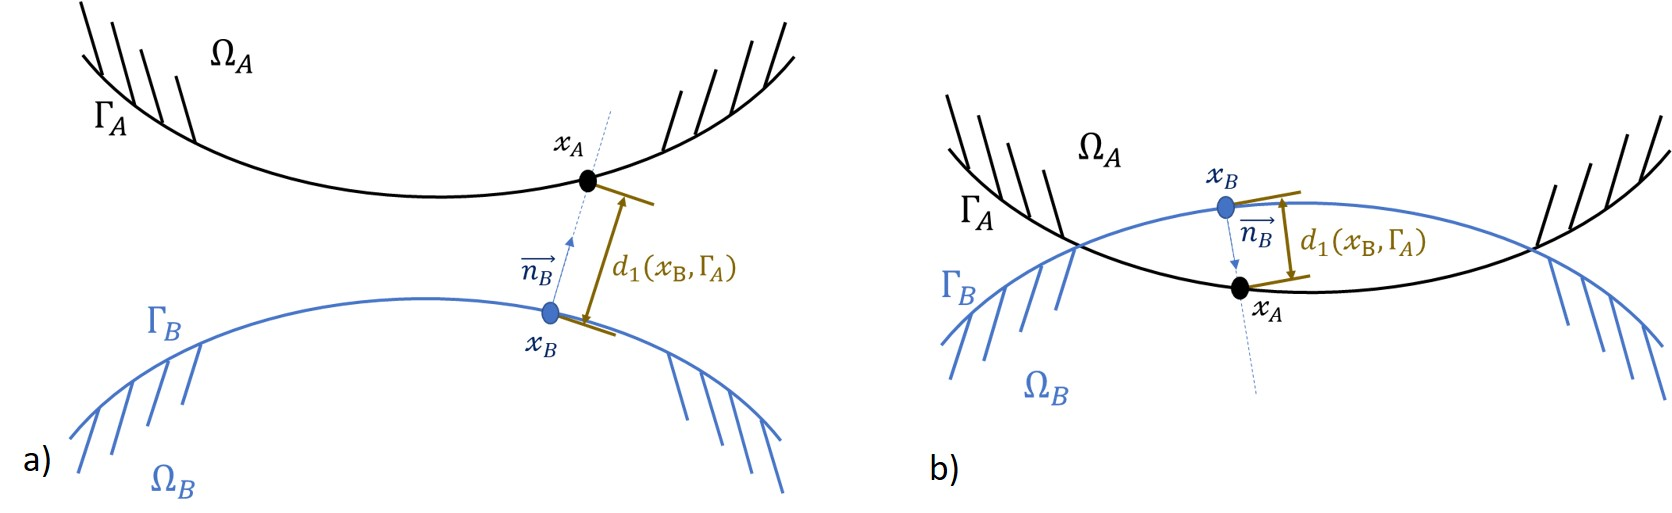
\includegraphics[width=1\textwidth,keepaspectratio]{figures/gap_penetration.jpg} }
\caption{a) Body $\mathcal{A}$ and body $\mathcal{B}$ are close but not in contact. The $d_1(x_B,\mathcal{A})$ measure define the gap between the bodies at point $x_B$.  b) Body $\mathcal{B}$ have penetrated the body $\mathcal{A}$. The $d_1(x_B,\mathcal{A})$ measure gives the penetration at point $x_B$.}
\label{gap_penetration}
\end{figure}
\end{center}

If the intersection point $x_A$ is located inside the pinball area, the node to surface distance define the amount of \textbf{gap} or \textbf{penetration} of the respective node (Figure \ref{gap_penetration}).
 
Computing the gap or penetration at single points increase numerical instabilities.  Therefore, in this work, the gap and penetration are computed in an averaged manner over the projected surface areas. Figure \ref{projecte_surface} show the projected surface areas (c) obtained by the intersection of the target surface areas (a) with the projected contact surface areas (b) over the target areas (a). 

 \begin{center}
\begin{figure}
\centerline{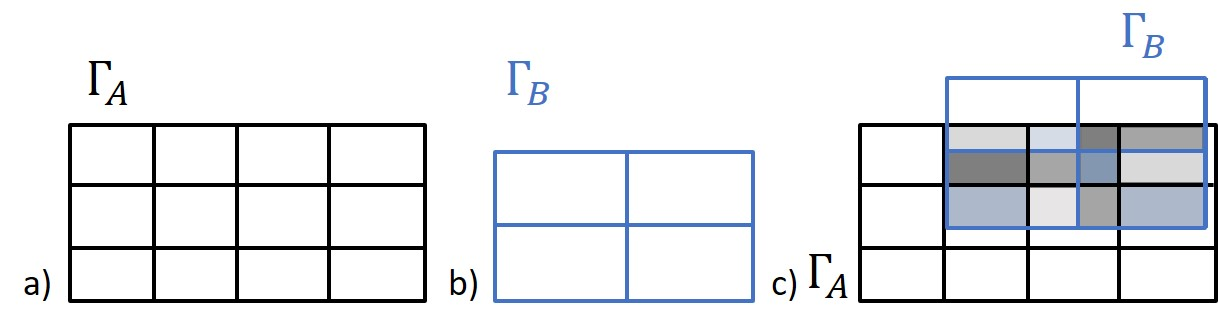
\includegraphics[width=1\textwidth,keepaspectratio]{figures/projecte_surface.jpg} }
\caption{The contact surface projection over the target surface: a) Target discretized area; b) contact discretized area; c) intersection of the projected surfaces.}
\label{projecte_surface}
\end{figure}
\end{center}

 The interested reader is referred to ANSYS contact technology guide \citep{ansys_contact_2017} for more details on the contact modeling.


\subsubsection*{Finite element mesh}
For the finite element computation, contact and target surfaces have to be discretized with 2D linear or quadratic elements (Figure \ref{discretization}) consistent with the underling 3D element mesh. The elements are named contact and target elements respectively.  They have no material properties apart the friction coefficient $\mu_f$. The stress-strain as well as the gap or penetration measures are computed for each mesh node of the discretized surface.

\subsubsection*{Pure Penalty method}
In this manuscript, one of the most popular mathematical expression of contact compatibility conditions is used, namely the penalty method. With such a method, additional contact properties are defined to manage contact behavior: a normal stiffness factor, opening stiffness factor, and a tangential stiffness factor. Such factors play an important role in the numerical computation but have no physical meaning.

The penalty method uses a spring like relationship to introduce a force for all nodes pairs (contact-target) that are defined to be in closed contact (Figure \ref{normalContactdistance}). The contact force is computed using the following expression:
\begin{equation}
f_c = k_c d
\end{equation}
where $d$ represents the penetration or gap amount and $k_c$ is the normal stiffness factor or the opening stiffness factor respectively. The tangential stiffness factor works in the same way enforcing the responding frictional force. Even if physical contacting bodies do not interpenetrate ($d = 0$), some finite amount of penetration, $d > 0$, is required mathematically to maintain equilibrium. 
 
 The biggest challenge here is that the magnitude of the stiffness contact factors is completely unknown beforehand. The contact force at each node have to be large enough to push the contact surface back to the target surface and eliminate unwanted penetration or gap. In the same time, if the contact force is too large, it pushes the contact surface far away from the pinball region causing error and solution instabilities.

\section{Breast biomechanical model: overview}

Biomechanical modelling of breast tissues has been widely investigated for various medical applications such as surgical procedure training, pre-operative planning, diagnosis and clinical biopsy, image guided surgery, image registration, and material parameter estimation (Table \ref{table:mechanical_models_table}). For the last 20 years, several research groups have presented their breast models based on finite elements modeling.  The complexity and relevance to breast anatomy of each model depend on the research purposes for which it was designed. 

Several groups have proposed biomechanical breast models to register uncompressed volumetric breast data to the compressed one \citep{han_development_2012,ruiter_model_based_2006,sturgeon_finite_element_2016} or to compressed projection mammographic data \citep{kellner_simulation_2007}. Within this framework, the authors modeled the breast deformation from prone to compressed prone position assuming linear elastic materials, zero residual stress and Dirichlet boundary conditions.
However, compression-like breast deformation is too limited to characterize global breast mechanics.

 Applications such as image guided surgery or preoperative planning imply a wider range of deformations. Therefore biomechanical breast models capable of estimating gravity induced deformation between different body position were proposed, for example from supine to prone positions (named also multi-loading gravity simulations) \citep{gamage_modelling_2012,georgii_simulation_2016,eiben_surface_2016} . Considering the involved large deformation, these models need to be more accurate with respect to mechanical and anatomical breast properties. In this respect, a patient-specific model is needed considering more personalized boundary conditions, material models and a better representation of breast anatomy. 

 
As described in Section \ref{section:continuousmechanics}, to build such a mechanical breast model, one need to provide the breast geometry in a \textbf{reference configuration}, the \textbf{constitutive models} of tissues composing the volume and the \textbf{boundary conditions}. The definition of all these variables has a significant impact on model accuracy.

\subsection{Breast reference configuration} 

A large number of existing patient specific models are using volumetric data from MR images \cite{carter_biomechanical_2009},\cite{kellner_simulation_2007}, \cite{conley_realization_2015} \cite{eiben_symmetric_2016}, \cite{martinez_finite_2017}  or CT images \cite{palomar_finite_2008},\cite{sturgeon_finite_element_2016} to design the breast geometry. During such exams, the acquired breast tissues are already deformed with deformation that significantly change breast geometries, for example if the patient is in a supine or in a prone position. Moreover, the deformed breast configurations include already the initial pre-stresses which are generally unknown and are extremely difficult to measure in clinical conditions. 
 

To model the breast tissues deformation under gravity loading, the reference state is chosen to be the breast geometry in a stress-free configuration, i.e. without being deformed by any force, including gravity. The breast stress-free geometry is practically impossible to measure; therefore, several estimation methods have been proposed. The four most used ones are described below.

 
 
  \subsubsection*{Inverse gravity}\label{subsubsection:inversegravity}
 \citep{palomar_finite_2008, sturgeon_finite_element_2016} used the inverse gravity method to estimate the stress-free geometry from the prone position measured during the exam. In their work, the authors just reversed the gravity effects without considering the initial stresses already included in the breast prone configuration. According to \cite{eiben_breast_2014} the inverse gravity methods gives a poor approximation of the breast reference state and can be used only with small deformations or highly constrained models.  

 \subsubsection*{Breast neutral buoyancy configuration}
 Assuming that breast density is equal to water density, \cite{rajagopal_creating_2008} compute the breast stress-free configuration by imaging the breast immersed in water. Following the same physical assumptions, \cite{kuhlmann_mechanical_2013} proposed to estimate the stress-free configuration by applying a hydro-static distributed load on the breast surface collected in a prone configuration. Even though the estimated geometries are accurate enough, these methods are time-consuming and is difficult to transpose in a clinical framework. 

 \subsubsection*{Prediction-correction iterative algorithm}
 The prediction-correction iterative method was first proposed by \citep{govindjee_computational_1998} and adapted later by \cite{carter_biomechanical_2009} and \cite{eiben_breast_2014}. The original method is based on the prediction-correction iterative scheme represented in Figure \ref{predictioncorectionalgo}. The first approximation of the breast reference configuration is estimated by applying the inverse gravity method on the prone breast configuration (see above).  Then, a numerical breast prone configuration is computed and compared to the corresponding measured one. The difference between the two prone geometries (The measured one and the simulated one) is used to update the reference breast configuration. The process is repeated until the convergence is achieved (i.e. then the difference is minimal). These methods were validated using the neutral buoyancy breast shape.

\begin{figure}[!h]
\centering
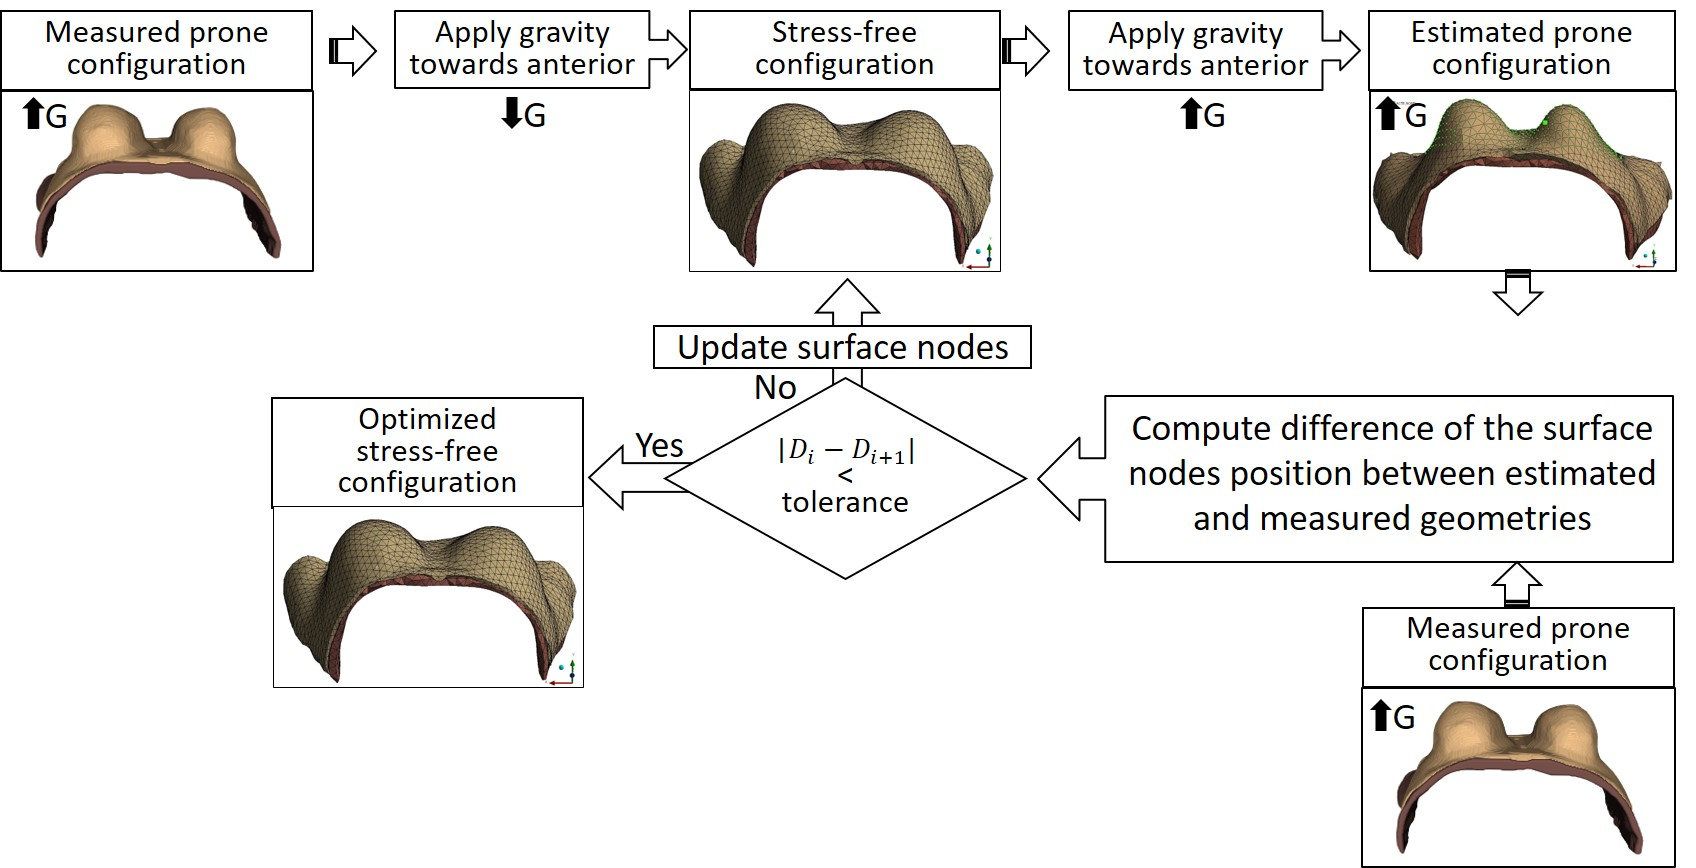
\includegraphics[width=1\textwidth,keepaspectratio]{figures/prediction-correction.jpg} 
\caption{Prediction-correction algorithm}\label{predictioncorectionalgo}
\end{figure}


 \subsubsection*{Inverse FE algorithm}
\cite{pathmanathan_predicting_2008} and later \cite{vavourakis_inverse_2016} proposed an analytic computation of the breast reference state by reparametrizing the equilibrium equation and by solving a finite element formulation of the inverse motion. The model provides good estimates of breast reference configurations but needs large numerical resources. \cite{eiben_breast_2014} showed that the prediction-correction iterative algorithm and the inverse FE algorithm are similar in terms of resulting accuracy. 

\subsection{Constitutive models}

Global breast mechanics is governed by breast tissue compositions and their individual mechanical properties. The breast soft tissues are known to be incompressible, nonlinear, anisotropic, and viscous materials. However, according to \cite{wellman_breast_1999} the breast tissues viscosity can be neglected when the mechanical load is applied within short time scales.  

Under large compression and body position changes, the breast volume can vary due to blood flows. Thus, soft tissues are frequently modeled as quasi-incompressible materials with a Poisson ratio ranging between $\nu = {0.45-0.5}$. The influence of the Poisson ratio within linear constitutive models was studied for breast by \cite{tanner_factors_2006}; according to the authors, the best estimates are obtained with high Poisson ratio ($\nu = {0.495,0.499}$). The breast tissues are predominately composed of water; therefore, the density is considered to be equal to $981\ kg/m^3$.  


For the last decades several constitutive models were used to model the breast tissues response to an external force: exponential elastic \citep{azar_methods_2002}, Neo-Hookean hyper-elastic \citep{carter_biomechanical_2009,rajagopal_modeling_2010,sturgeon_finite_element_2016, eiben_breast_2016, han_nonlinear_2014, garcia_mapping_2017}, Money-Rivlin \citep{samani_elastic_2007,tanner_factors_2006,carter_application_2012,martinez_finite_2017}. \cite{eder_comparison_2014} compared the most popular models in a multi-loading gravity simulation; according to the authors, the Neo-Hookean model proposed by \cite{rajagopal_creating_2008} gives the best estimates.

\subsubsection*{Glandular and adipose tissues biomechanical properties }
 Multiple studies have shown that breast composition, and so its mechanical behavior undergo substantial changes during woman lifetime (section \ref{subsection:adultbreasttexturechanges}). The first studies on mechanical proprieties estimation of breast tissues were done in diagnosis purposes. When the breast is developing benign or malign disorders, its mechanical properties differ from the ones of the normal breast tissues.  In a study of 142 samples, bellowing to 4 type of tissues, \cite{krouskop_elastic_1998} found that depending on the pre-compression level, Young moduli of invasive carcinoma is from 5 to 25 times larger than the one of normal adipose tissue  ( from 5\% to 20\% strain levels).  

Later, several research groups (Table \ref{table:materialproperties}) have studied the elastic moduli of adipose and glandular tissues. The breast tissues elastic parameters range between 0.1 kPa and 271.8 kPa. Such huge variation may be explained by the differences in the experimental set-up used to estimate stiffness, but also by the participant's physical condition, age or period of the menstrual cycle. For example, \cite{han_development_2012}, though using the same FE method, found significantly inter-individual variability, with the shear moduli ranging between $0.22-43.64 kPa$. \cite{lorenzen_menstrual-cycle_2003} showed that during the menstrual cycle, due to the hormonal changes, the elastic properties of the glandular tissues can change by about 30\%.

\begin{table}[!h]
\centering
\begin{tabular}{|p{0.25\linewidth}|p{0.13\linewidth}|p{0.1\linewidth}|p{0.17\linewidth}|p{0.17\linewidth}|}
 \hline
\multicolumn{5}{|c|}{\textbf{Ex-vivo estimation}}\\ \hline

\multirow{2}{*}{ Author} & \multirow{2}{*}{ Method} &  Material & \multicolumn{2}{c|}{material properties}\\  \cline{4-5}

&& model &Adipose $kPa$ & Glandular $kPa$ \\  \hline

\cite{krouskop_elastic_1998} & Indentation-5\% . & Linear elastic & $\lambda=19 \pm 7\ kPa$ &$ \lambda =33 \pm 11\ kPa$ \\ \hline
 \cite{krouskop_elastic_1998}   & Indentation- 20\%& Linear elastic & $\lambda=20 \pm 6\ kPa  $& $\lambda= 57 \pm 19\ kPa $ \\  \hline
 \cite{wellman_breast_1999}  & Indentation - 5\% & Linear elastic & $\lambda=6.6\ kPa $ & $\lambda= 33 \ kPa$\\ \hline
 \cite{wellman_breast_1999}  & Indentation - 15\% & Linear elastic &$ \lambda = 17.4\ kPa $& $\lambda= 271.8\ kPa $ \\ \hline
 \cite{azar_methods_2002} & Indentation & Exp. elastic & $b = 4.46\ kPa$; $m=7.4$ & $b = 15.1\ kPa$; $m=10$ \\ \hline
 \cite{samani_method_2004} & Indentation & Linear elastic & $\lambda= 3.25 \pm 0.91\ kPa $ & $\lambda= 3.24 \pm 0.61\ kPa $ \\ \hline \hline
 \multicolumn{5}{|c|}{\textbf{In-vivo estimation}}\\ \hline
 \cite{van_initial_2003} & MRE & Linear elastic & $\lambda= 17-26\ kPa $ & $\lambda= 26-30\ kPa $ \\ \hline
 \cite{sinkus_viscoelastic_2005}&MRE& Visco-elastic & \multicolumn{2}{|c|}{$\mu = 2.9 \pm 0.3\ kPa$} \\ \hline
 \cite{rajagopal_creating_2008}  & MRI-FEM& Neo-Hookean & $\mu = 0.16$\ kPa & $\mu = 0.26\ kPa$ \\ \hline
 \cite{carter_determining_2009} & MRI-FEM& Neo-Hookean &$\mu = 0.25\ kPa$ & $\mu = 0.4\ kPa$ \\ \hline
 \cite{han_development_2012} & MRI-FEM & Neo-Hookean & $\lambda= 1\ kPa$ & $\lambda = 0.22-43.64\ kPa $ \\ \hline 
 \cite{gamage_modelling_2012} & MRI-FEM & Neo-Hookean & \multicolumn{2}{|c|}{$\mu = 0.1\ kPa $} \\ \hline
 \cite{griesenauer_breast_2017} & MRI-FEM & Hooks law & $\lambda= 0.25\ kPa$ & $\lambda= 2\ kPa$\\ \hline
\end{tabular}
\caption{Material properties for adipose and glandular tissues.}
\label{table:materialproperties}
\end{table}

An important difference in estimated values of breast elastic moduli is observed between the linear elastic and hyperelastic models. If only in-vivo studies with Neo-Hookean material models are considered, the range of the adipose and glandular shear moduli is significantly lower than $ 50kPa$. 

\cite{carter_biomechanical_2009} compared a one parameter Neo-Hookean potential function with a five parameters Money-Rivlin potential function for various material properties. The multi-loading gravity simulations were thus performed on 3 subjects. According to the authors, even for parameters 10 times softer than the literature \citep{abbas_biomechanical_2001}, the Money-Rivlin model underestimates the tissues deformation by at least 75\% when the subject is re-positioned from the supine to the prone positions. The best estimates were given by the Neo-Hookean model with the initial shear moduli equal to $0.2kPa$.  

Previously listed researches clearly showed the variability of elastic moduli of the same tissue between and within individuals. \cite{eder_comparison_2014} made a larger analysis including all material models proposed in the literature. According to authors, many of them are too stiff permitting not enough deformation within the gravity loading. This study has shown that the most reliable elastic moduli values are the ones given by \cite{rajagopal_creating_2008} (Table \ref{table:materialproperties}).

\subsubsection*{Muscle biomechanical properties.} 
Muscle is a kinematically, geometrically, and materially complex tissue. Muscle mechanical behavior depends on its contractile active and passive elastic properties \citep{nordez_muscle_2010}. In biomechanics the muscle is modeled using complex models as Hill-type models
\citep{zajac_muscle_1989}, Feldman’s lambda model \citep{feldman_once_1986} which are considering the variation of muscle elasticity in function of muscle state. In breast biomechanical models the muscle is combined with the thoracic cage and is frequently considered as a rigid breast support. In most of models, the pectoral muscle is modeled by imposing zero-displacement conditions on nodes closer to the chest wall \citep{abbas_biomechanical_2001,chung_modelling_2008,rajagopal_mapping_2010}  
or by allowing them to slide along the chest wall line \citep{han_nonlinear_2014,georgii_simulation_2016}.   

The muscle is nonlinear, anisotropic, incompressible material.  The bibliographic data on static mechanical properties of the muscle-tendon unit assessed by supersonic shear wave imaging elastography state a Young's modullus in range of $20kPa$ to $300kPa$ depending on the muscle location and subject's physical condition \citep{lima_eassessment_2018}.  The muscle shear moduli on the upper trapezius was studied by \cite{leong_quantitative_2013}, according to authors the muscle shear elasticity at rest was $17.11\pm 5.82 kPa$, and this increased to $26.56\pm 12.32 kPa$ during active arm holding at 30\textdegree  abduction. 

\subsubsection*{Skin biomechanical properties}
Several studies have shown the importance of skin in biomechanical breast modeling. According to \cite{carter_biomechanical_2009}, a model which includes the skin estimates better the tissues deformation under gravity loading.

 \cite{sutradhar_vivo_2013} published a complete study of breast skin estimating its elasticity for 16 different breast regions. The study was done on 23 female volunteers aging from 29 to 75 years. The authors found that the skin elastic moduli range between $15-480 kPa$ with an average of $334\pm 88 kPa$. The elastic moduli in the lateral region (mean $370 kPa$) has the highest value followed by the superior region (mean $355 kPa$); the inferior region (mean $331 kPa$) follows next, with the medial region having the
lowest value (mean $316 kPa$). However, no significant variation of elastic moduli in radial direction was found. 
 
Other researches on skin elasticity are available, but they are not specific to the breast skin. \cite{hendriks_relative_2006} estimated in-vivo skin properties by suction testing. The skin was considered as a homogeneous, isotropic, incompressible, hyperelastic material. The study was performed on 14 subjects and the obtained average of elastic moduli for skin was $58.4 kPa$.

The estimation of the breast skin elasticity by the means of finite elements using Neo-Hookean potential function has resulted in softer materials model. \cite{carter_determining_2009} found an initial shear modulus equal to $16kPa$, whereas \cite{han_nonlinear_2014} found that for the five studied subjects the skin shear moduli ranged between $2.47 kPa$ and $5.78kPa$. 

\subsubsection*{Fascias and ligaments biomechanical properties}
The surrounding breast fascias and the supervisory ligament form the breast support matrix. These structures are well described for surgical purposes (thickness, location etc), however little is known about their mechanical properties. The first biomechanical breast model taking into account the effect of Cooper's ligaments was proposed by \cite{azar_methods_2002} and took up later by \cite{pathmanathan_predicting_2008} and \cite{han_development_2012}. The authors designed a new material model for fatty tissues including the anisotropic behavior of breast ligaments. Later, \cite{georgii_simulation_2016} come up with a spring-mass generic model for the breast support matrix. According to the authors, including the ligaments into the finite elements breast model have increased the robustness of the prone-supine simulation with respect to the input parameters. 

 To our knowledge, where are no experimental data describing the mechanical properties of breast superficial fascia. An approximation of the elastic moduli of Cooper's ligaments is given by \cite{gefen_mechanics_2007} by extrapolating from known ligamentous structure in the human body. The authors estimated the elastic moduli of suspensory ligaments to relay between $80 - 400 MPa$
 
 %microscopic and macroscopic study of fascia
 Fibrous tissues get their elasticity from elastin elastic fibers and their structural support from collagen fibers. As reported by \cite{riggio_anatomical_2000}, the superficial fascia is made up of both collagen and elastin fibers. In contrast, the Cooper's ligaments appeared to be composed almost of collagen fibers.  The mechanical properties of a single collagen fiber from a rat tail were studied by \cite{wenger_mechanical_2007}; according to the authors the corresponding elastic moduli range between $5 GPa$ and $11 GPa$. Other studies on biomechanical characterization of human body superficial fascia are available in the literature. The most frequently studied structures are the plantar fascia and foot ligaments, with a Young's moduli ranging between $0.1e^{-3} MPa$ \citep{gefen_vivo_2003} and $700 MPa$ \citep{cheung_effects_2004}. 

\subsection{Boundary conditions}

Dirichlet conditions are usually used to constrain the sternum/axilla ends and the posterior surface of the breast or the thoracic cage if the muscular tissues are considered \citep{griesenauer_breast_2017,rajagopal_creating_2008,pathmanathan_predicting_2008, gamage_modelling_2012,griesenauer_breast_2017}. As reported by \cite{carter_biomechanical_2009} the zero-displacement boundary conditions in a multi-gravity loading framework result in an over-constrained model; in that case sliding conditions on the mesh nodes corresponding to the chest wall have to be considered.    

  Later, several teams using biomechanical breast models for multy modality image registration or surgical planing showed that including the sliding boundary conditions \citep{georgii_simulation_2016,han_nonlinear_2014}  improves the registration accuracy. However the most studies in which the biomechanical model is designed for breast compression, the tissues sliding over the chest wall is neglected and fixed boundary conditions are usually assumed \citep{sturgeon_finite_element_2016, martinez_finite_2017}.
  
 \subsection{Summary}
 
 During the last decades, several breast biomechanical models were proposed. However, only a small part of them \citep{carter_biomechanical_2009,gamage_modelling_2012,han_nonlinear_2014} were evaluated with respect to real tissues deformations. As we intend to build-up a subject specific breast biomechanical model capable of estimating multi-loading gravity deformations, we will only consider as relevant the biomechanical models that were evaluated and compared with real data. In this chapter, three biggest challenges were identified:  the estimation of the breast reference geometry, the estimation of patient specific material properties and the definition of the boundary condition and namely the breast-muscle interface. Today's outstanding breast biomechanical models are represented by the next three models:   \cite{eiben_surface_2016}, \cite{han_nonlinear_2014}, \cite{gamage_modelling_2012}.   

 \cite{gamage_modelling_2012} proposed a finite elements model capable to estimate the supine breast configuration from the prone one. The breast stress-free configuration was estimated using a prediction-correction iterative algorithm optimization process, in this purpose the skin surfaces on prone configuration was used as ground-truth. Contrariwise, the material constitutive parameters were identified using the skin surface on supine breast configuration by applying a non-linear optimization algorithm. Breast tissues sliding over the chest wall was considered partially by modeling the pectoral muscle as a soft structure and including it into the optimization process. The models were evaluated for the supine breast configuration by computing the root-mean-squared error (RMSE) from the point to surface distance between the estimated and measured data. Conform to the authors, the breast supine geometry was estimated within an RMSE of 5mm (maximal distance of 9.3 mm). 

In the same time, \cite{han_nonlinear_2014} developed a breast biomechanical model for image registration. The estimates of supine breast configuration were computed for five subjects, and the accuracy was assessed by computing the Euclidian distance between anatomical landmarks.  The mean Euclidian distance range between 11.5 mm and 39.2 mm (maximal Euclidian distance ranged between 20.3mm and 61.7mm). The authors modelled the elongation of the pectoral muscle using a contact sliding model. Only the material constitutive parameters were adapted to the patient’s breast mechanics, the stress-free breast geometry being estimated by inverse gravity. 

Finally, \cite{eiben_surface_2016} proposed a new model to estimate the up-standing breast configuration from the prone one. The model was evaluated on 3 subject. The patient specific stress-free geometry was computed using an inverse finite elements u-p formulation. The material parameters were optimized such that the best fit in supine configuration is obtained. The estimates quality was measured in terms of the mean Eulerian Distance between manually selected internal landmarks. Thus, the supine breast configuration was estimated within a mean distance ranging between $12.2mm$ and $19.8 mm$. The model evaluation for the up-standing configuration was not presented.

A new biomechanical breast model is proposed in the next chapter considering the patient specific breast geometry and elastic properties as proposed by the previous models. In addition, the breast tissues sliding over the chest wall is modeled by including new anatomical structures as superficial fascia and suspensory ligaments. We believe that global breast mechanics are driven by these stiff structures. Finally, the model will be evaluated by confrontation with real data collected from MR images.        
 
 
\begin{sidewaystable}[!h]
    \centering
    \small
   \begin{tabularx}{22cm}{|p{2.5cm}|p{2.5cm}|p{3.5cm}|X|p{3.5cm}|p{2.5cm}|}
   \hline
   Authors & Application & FE mesh & Material models & Boundary conditions & Stress-free config. \\
\hline
  Azar F. et al. \citep{azar_methods_2002} &  Computer assisted breast surgery & 8-Node hexahedrons (trilinear isotropic elements) & Skin-elastic linear, 
   adipose,glamdular-hyperelastic polynomial & Sliding between breast - thorax and breast-paddle & Prone breast geometry\\
   \hline
 Rajagopal V. et al.  \citep{rajagopal_modelling_2007} & Breast compression & 8-Node hexahedrons (tricubic Hermite elements)& Homogeneous , Neo-Hookean model& Zero-displacement BC & Buoyant breast in water \\
   \hline
  Pathmanathan P. et al. \citep{pathmanathan_predicting_2008}&Image registration & 8-Node hexahedrons (trilinear elements)& Homogeneous breast-polynomial hyperelastic; Skin exponential hyperelastic  & Zero-displacement on muscle; Compression with imposed displacement & Inverse FE algorithm \\
   \hline
  Han L. et al. \citep{han_nonlinear_2014}& Image registration& 4-Node tetrahedrons & Muscle, glandular, fatty, skin - Neo-Hookean model & Sliding on pectoral muscle & Inverse gravity \\
   \hline
 Gamage T. et al.  \citep{gamage_modelling_2012}&  Computer assisted breast surgery & 8-Node hexahedrons (tricubic Hermite elements) & Homogeneous+ muscle- Neo-Hookean incompressible model& Zero-displacement BC on rib cage surface, Sternum, axilla ends, shoulder & PC iterative algorithm \\
   \hline
 Patete P. et al.  \cite{patete_multi_2013}& Computer assisted breast surgery& 4-Node tetrahedrons (trilinear isotropic elements) & Adipose , glandular, skin & Zero-displacement BC on the  chest wall&PC iterative algorithm\\
   \hline
 Kuhlmann M. et al. \citep{kuhlmann_mechanical_2013}& image registration & 4-Node tetrahedrons & Adipose, glandular- linear gel-like (Eulerian formulation); Skin - hyperelastic material (Lagrangian formulation) & Zero-displacement chest wall& PC iterative algorithm\\
   \hline
   
 Georgii J. et al.  \citep{georgii_simulation_2016}&Surgery simulation & 8-Node hexahedrons, 2-node 3D spars & homogeneous elastic material, Cooper's ligaments-generic mass-spring model & sliding BC (breast on the pectoral muscle) & NA\\
   \hline
  Eiben B. et al. \citep{eiben_surface_2016} & Surgery outcome prediction & 4-Node tetrahedrons & Fatty , glandular- Neo-Hookean model; skin- exponential hyperelastic & Zero-displacement BC & Inverse FE algorithm \\ 
   \hline
  Garcia E. et al. \citep{garcia_mapping_2017} & 3D breast lesion localization & 4-Node tetrahedrons & adipose, glandular  - Neo-Hookean models &zero-displacement BC & Prone breast configuration\\
   \hline
    \end{tabularx}
     \caption{Breast biomechanical models}
     \label{table:mechanical_models_table}
\end{sidewaystable}


%\end{table}



\chapter{A new biomechanical breast model}\label{chapter:myBioMecaModel}
\input{chapters/mybioMecaModel}
\chapter{Model validation}\label{chapter:modelvalidation}

\section{Technical approach}\label{section:validation:technical approach}





\section{Results}\label{section:multi-loadinggravityvalidation}



\begin{figure}[!h]
\centering
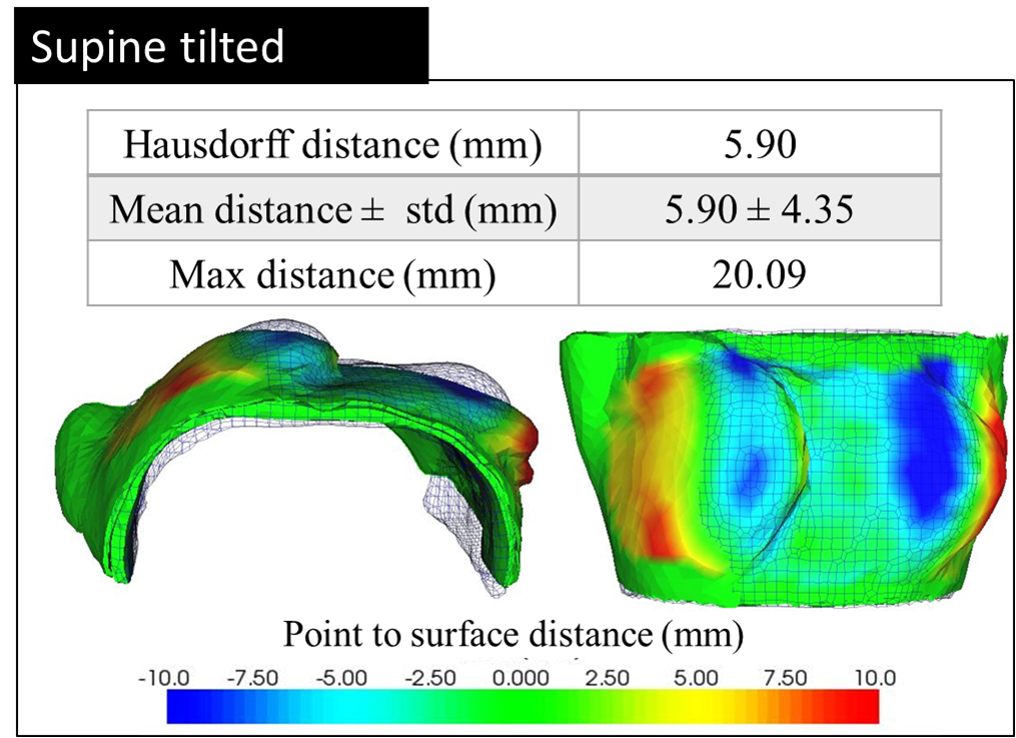
\includegraphics[width=0.9\textwidth,keepaspectratio]{figures/modelevaluation.png} 
\caption{Three breast configurations: prone, supine and supine tilted. First line - MR images in 3 breast configurations. Second and third lines - point to node distance from simulated breast shape (surface mesh) to the measured one (black grid lines).}\label{fig:modelevaluation}
\end{figure}

{\color{darkblue} Add the results with Gent model and compare}

\section{Discussions and conclusion} \label{section:validation:discutionconclusion}


\clearemptydoublepage
\part{Breast Compression: a comparative study}\label{part:breastcompressionDM}
\chapter{ Background }\label{chapter:compression:introduction}


Mammography is the sole breast cancer screening method recognized by the European Commission for women aged 50-69 years. This method enables examination of the breast in its entirety and offers a high sensitivity for early-stage tumors. However, the mammographic exam is known to be unpleasant for the patient, the main source of discomfort being related to breast compression.  For such a standardized and wide-used procedure, good exam conditions and patient comfort should be ensured. Therefore, a study on the relevance of breast compression in mammography is of a potential interest.\\



 This chapter describes the standard mammographic procedure, including the breast positioning methods and the design of the most used paddles. The need of compression is explained in terms of image quality and average glandular dose. Patient comfort and the respective current gold standards are introduced. Finally, the interest of developing a simulation environment to assess the quality of breast compression is explained.

\clearpage
\section{Mammography positioning} \label{subsec:mammographicpositioning}

During the mammography exam, a qualified radiology technologist positions the breast of the patient between the stationary image receptor and a movable paddle. A routine screening mammography exam consists of two views per breast: cranio-caudal (CC\nomenclature{CC}{Cranio-Caudal view}) and mediolateral oblique (MLO\nomenclature{MLO}{Mediolateral Oblique view}) projections.  

In a regular workflow, the breast compression is performed in the up-right body position. In the CC view ( Figure \ref{fig:cc_mlo_view} left) the breast is placed on the image receptor, that is initially positioned at the inframammary fold level or a few centimeters higher depending on breast mobility. Then, the technologist lowers the compression paddle using a foot switch while gently pulling and positioning the breast onto the image receptor to maximize the amount of projected tissues in the image. In the MLO view ( Figure  \ref{fig:cc_mlo_view} right), the image receptor is rotated to an angle between 40 to 55 deg. The lateral oblique side of the breast is positioned against the image receptor. In this view the pectoral muscle is located between the detector and the compression paddle; as the muscle is stiffer than the breast tissue, the woman has to stay relaxed in order to get a better breast flattening. When lowering the compression paddle, the technologist has to pull the breast upward and forward to prevent breast drooping, and to smooth out any skin folds. 


\begin{figure}[!h]
\centering
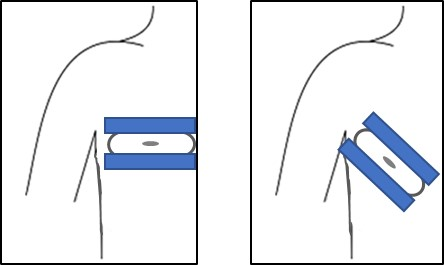
\includegraphics[width=0.5\textwidth,keepaspectratio]{figures/cc_mlo_view.jpg} 
\caption{left: cranio-caudal breast compression; righ: mediolateral oblique breast compression. }
\label{fig:cc_mlo_view}
\end{figure}

 The two views are complementary. The MLO view covers a large amount of tissue and provides a better visualization of the upper juxtathoracic part of the breast, while the CC-view suffers less from overlapping dense tissue and provides a better visualization on the central part of the breast \citep{chan_image_1987,kim_computer_2006}.  Further incidences or magnification views may be needed for diagnostic mammography \citep{groot_towards_2015}.
 

The mammography devices are equipped with paddle position and force sensors to measure and display the compressed breast thickness and the amount of force applied to the breast.

\section{Paddles designs} \label{section:compressionpaddlesdesign}

Nowadays, a wide range of compression paddles are available for breast clinical examination. Their shape and dimensions vary in function of the purpose for which they were designed but also from manufacturer to manufacturer. According to their specific
indications of use, three categories can be distinguished: \textbf{standard paddle} used for regular screening, \textbf{spot paddles} used for diagnosis purposes, and \textbf{biopsy paddles} used for breast compression during breast biopsy (Figure \ref{fig:compressionpaddlestypes}). 


\begin{figure}[!h]
\centering
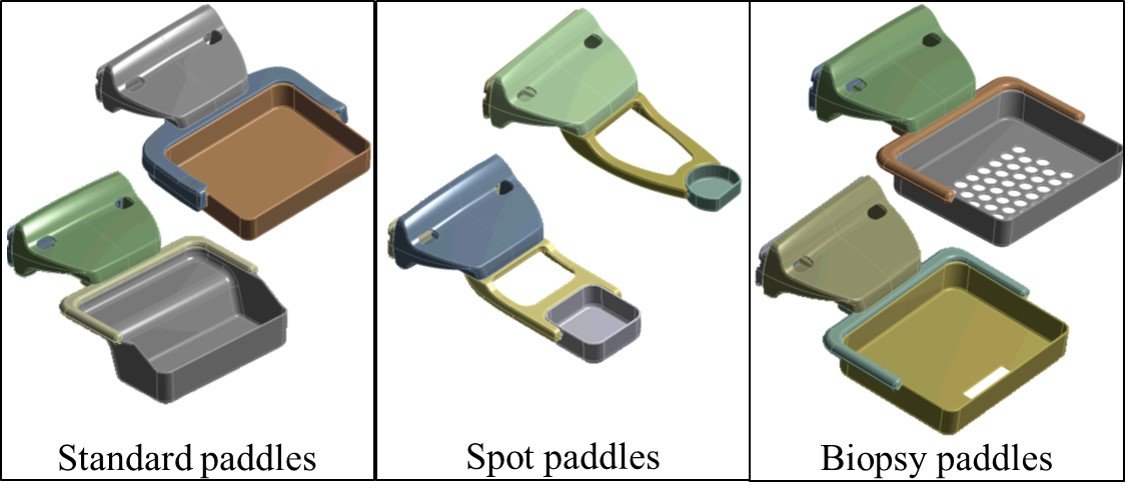
\includegraphics[width=0.9\textwidth,keepaspectratio]{figures/compressionpaddlestypes.jpg} 
\caption{Different breast compression paddles for GE Healthcare mammography units .}\label{fig:compressionpaddlestypes}
\end{figure}
    

 The standard compression paddles have usually a rectangular shape with a flat compression plate. Depending on the industrial manufacturer, they can have different sizes for both the lateral and longitudinal edges and for the paddle front edge height. Paddles with smaller compression area are used to compress small breasts or breasts with implants (Figure \ref{fig:compressionpaddlestypes}, Standard paddles). Standard paddles are classified into rigid and flexible paddles. The standard rigid paddle (SRP)\nomenclature{SRP}{ Standard Rigid Paddle} is fixed to its frame and is constrained to move in the up-down direction only. This paddle has some flexibility because of its material mechanical properties and can slightly bend when compressing the breast, while remaining globally parallel to the image receptor (Figure \ref{fig:compressionpaddles}.b). On the other hand, the standard flex paddle (SFP) \nomenclature{SFP}{Standard Flex Paddles} is attached to its frame by flexible joints and therefore, presents an additional degree of freedom enabling the paddle to tilt with respect to the image receptor plane (Figure 3.c). During compression the paddle remains parallel to the detector at first, tilts towards nipple side and then ends with the highest point at the thorax level. Depending on the breast position, the paddle may also slightly tilt in the medio-lateral direction.

\begin{figure}[!h]
\centering
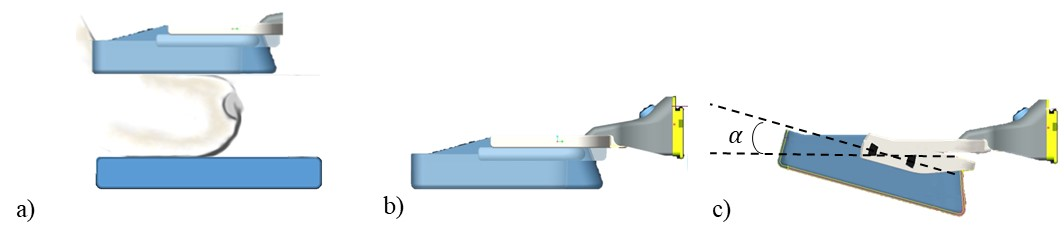
\includegraphics[width=0.9\textwidth,keepaspectratio]{figures/compressionpaddles.jpg} 
\caption{a) Breast compression between the paddle (up) and the image receptor (down): b) Rigid paddle; c)Flex paddle with a flexion angle $\alpha$}\label{fig:compressionpaddles}
\end{figure}


 Spot paddles apply the compression to a smaller area of tissue using a small compression plate or a cone. By applying compression to only a specific area of the breast, the effective pressure is increased on that spot. This results in a better tissue separation and allows for a better visualization of the small area in question.  It is used to distinguish between the presence of a true lesion and an overlap of tissues, as well as to better show the borders of an abnormality or questionable area or a little cluster of faint microcalcifications.  

Biopsy exams require that the patient's breast remain immobile and compressed during the entire procedure. The biopsy paddles have basically the same shape as the standard rigid paddles. However, to allow the needle insertion and the accessibility to the biopsied area, the paddle plate contains multiple holes with various diameter or a single aperture. 

In this chapter, only breast compression with the rigid paddle in the two main view (MLO and CC) is considered.

\section{Compression mechanics} \label{subsec:compressionmechanics}
Nowadays, the European Commission recommends a force standardized breast compression, i.e. a compression that stops at a level of force just below the subject's pain threshold or at the maximum force setting of the machine.  The compression guidelines state that force should be firm but tolerable with a maximum applied compression of 130-200 N \citep{perry_european_2008}. As there is no exact specification for the application of breast compression, the applied force may vary between technologists and radiologists. Mercer C. and colleagues \citep{mercer_practitioner_2013} have analyzed the variation of the applied force within 14 trained practitioners. Both views, CC and MLO, were included. The authors found a significant difference between the average applied forces and have highlighted three groups of radiologists depending on the mean force intensity. Between the consecutive groups, a mean difference of $16 \ N$ was found. 

The global breast compression cycle is characterized by two phases: flattening and clamping \citep{de_pain_2015}. During the flattening phase, the breast is gradually deformed by increasing the compression force; this step lasts about  $7.5 \pm 2.6\ s$. By contrast, during the clamping phase, which lasts approximately $12.8 \pm 3.6\ s$, the compression paddle is immobilized holding the breast in a stationary position. 
\begin{figure}[!h]
\centering
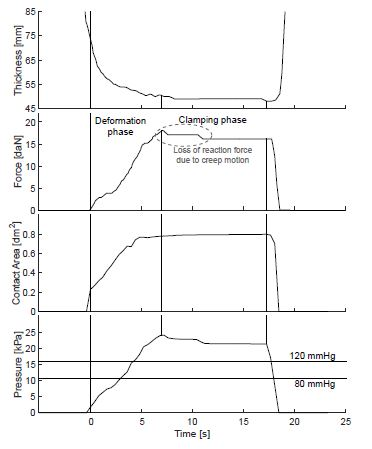
\includegraphics[width=0.7\textwidth,keepaspectratio]{figures/breast_compression_cycle.jpg} 
\caption{A typical breast compression cycle. Reproduced from Groot J.E. et al. \citep{groot_towards_2015}}\label{fig:breast_compression_cycle}
\end{figure}

Figure \ref{fig:breast_compression_cycle} shows a typical compression cycle for a CC breast compression from experimental data on real patients described by Groot J.E. et al. \citep{de_pain_2015}. One can see that, during compression phase, the breast thickness and contact area evolve non-linearly; meanwhile, the compression force and pressure increase quasi-linearly. During the clamping phase, the breast thickness remains constant; however, the skin pressure and the compression force slightly decreases in the first $10s$. This phenomenon may be explained by breast volume changes because of the viscous effusion of blood and lymph into the central systems. 

In the same work, the authors present several in-vivo measured patterns describing the relation between breast thickness and compression force depending on breast size and its firmness (Figure \ref{fig:thickness_force_patterns_groot}). One can see that, for a larger breast, higher compression force is needed but the overall behavior remains the same as for smaller breasts. For similar breast sizes, the final compression forces range within the same values, however a firmer breast will reach faster the limiting value of breast thickness resulting in an asymptotic increase of the compression force.
\begin{figure}[!h]
\centering
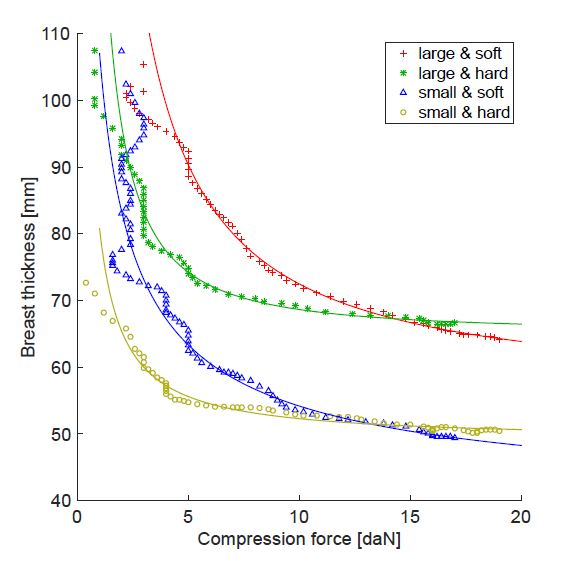
\includegraphics[width=0.6\textwidth,keepaspectratio]{figures/thickness_force_patterns_groot.jpg} 
\caption{In-vivo measured breast flattening curves as function of the applied force. Reproduced from Groot J.E. et al. \citep{groot_towards_2015}}\label{fig:thickness_force_patterns_groot}
\end{figure}

Dustler M. and colleagues \citep{dustler_breast_2012} have studied the pressure distribution patterns for MLO breast compression (55 degree tilt). The authors showed that the pressure distribution varies widely within the breast. The obtained patterns from 131 subjects were classified into four main groups: a) skin pressure widespread over the breast (29\%); b) skin pressure concentrated on the central part of the breast (8\%); c) skin pressure concentrated on the juxtathoracic region (16\%); d) skin pressure concentrated along a narrow zone at the juxtathoracic region (26\%). According to their results, the pressure distribution depends on two factors: the variation on breast thickness from one side and surrounding tissues stiffness from the other side. For example, for the groups c and d the breast anterior tissues compression is limited by the pectoral muscle which is much stiffer than the breast tissues.  These results may explain the fact that, in MLO view, the breast thickness exceeds the one on the CC view, despite the larger force used in MLO than in CC breast compression \citep{mercer_practitioner_2013, helvie_breast_1994}. 

\section{Compression quality metrics}
A standard mammography protocol always includes breast compression prior to image acquisition. The breast flattening improves diagnostic image quality and reduces the absorbed dose of ionizing photons. However, the discomfort and pain produced by this procedure sometimes might deter women from attending breast screening by mammography. 

An important improvement concerning the patient comfort could be achieved with the emergence of digital mammography. Indeed, several studies have shown that digital mammography is better in terms of image quality \citep{obenauer_screen_2002} and radiation dose \citep{chen_analysis_2012} than film-screen mammography.

Most digital mammography systems have an automatic beam quality selection mode (automatic optimization of parameters, AOP\nomenclature{AOP}{Automatic Optimization of Parameters}) with an automatic exposure control (AEC \nomenclature{AEC}{Automatic Exposure Control}). The AOP mode automatically selects the X-ray  tube  voltage, the anode  target  material  and  filter  material defining the X-ray spectrum, in order to optimize the \textit{contrast to dose ratio}, i.e. the appropriate amount of radiation for an acceptable low dose and an increased contrast, according to breast thickness and composition \citep{williams_optimization_2008}. Then, the required exposure time for the actual image is calculated by the AEC.  The AOP control allows to determine, for each patient and compression level, the X-ray spectrum that optimizes the  ratio of benefits  (higher image contrast) and  drawbacks  (higher  dose). 
In this section, the compression quality will be measured in terms of three metrics: image quality, average dose and patient comfort. A detailed description of each metric is given below with their impact for digital mammography. 

\subsection{Image quality}

Many factors may influence the quality of the mammography image such as the knowledge and skill of the person who performs the mammography examination, the equipment, the positioning
technique, and the compressed breast thickness, type of breast
cancer, and radiographic appearance of the breast tissue \citep{de_pain_2015,andolina2011mammographic}. In our study, only the impact of the compressed breast thickness on image quality is analyzed.

 Firstly, the breast compression facilitates the image interpretation. Higher compression leads to better tissues spread and consequently to less overlapping of clinical important structures. A thinner layer of breast tissues allows a more subtle differentiation between normal and suspicious findings. Secondly, breast compression affects the image sharpness. Since the exposure time lasts several seconds, a proper breast immobilization reduces the image blurring, preserving the conspicuity of abnormal legions. Moreover, with a reduced breast thickness, the primary contrast is raised due to the reduction of radiation scatter to primary ratio at detector level. Finally, the breast compression leads to a better use of the detector dynamic range. With a non-uniform breast thickness, the different levels of brightness are used to describe the thickness variation, thus the detector dynamic is not used optimally for the contrast representation due to different internal structures. This is particular true for screen-film technology, with digital detectors; this constraint can be challenged.

It has been proved that image quality decreases with increasing breast thickness \citep{ko_dose_2013,helvie_breast_1994,saunders_effect_2008,poulos_breast_2003}. Helvie M. and colleagues \citep{helvie_breast_1994} analyzed the image quality for the observed breast thickness of 250 subjects using film-screen mammography.  The difference in breast thickness and image quality between the MLO and CC paired images were computed. According to the authors, image sharpness decreased by 19\% for $1\ cm$ of increased breast thickness. In addition, contrast loss was observed due to scatter augmentation and beam hardening.

Later, Saunders R.S. et al. \citep{saunders_effect_2008} have studied the effect of breast compression on mass conspicuity in digital mammography using Monte Carlo based simulation framework. The simulation was done for two breast thicknesses $(4\ cm\ and\ 6\ cm)$ with two compression levels (standard and reduced compression by $12\%$) and three photon flux conditions (constant
flux, constant detector signal, and constant glandular dose). The results suggest that if a particular imaging system can handle an approximately 10\% increase in total tube output and 10\% decrease in detector signal, breast compression can be reduced by about 12\% in terms of breast thickness with little impact on image quality or dose.

O'Leary D. et al. \cite{oleary_compression_2011} performed a clinical study to assess the image quality in function of the applied compression force for digital mammography. The CC and MLO views of 4790 subjects were analyzed and image quality was categorized as  perfect, good, moderate or
inadequate. The results have shown that the image quality is highly correlated with the applied force. The mean compression force required to produce a perfect image was found to be equal to 121.34 N for a CC view and 134.23 N for a MLO view.

\subsection{Average glandular dose}
A mammography unit uses X-rays to obtain 2D-projection images from the breast tissues. As for any X-ray exposure, the irradiation of a targeted population is accepted if the benefits are significantly higher than the risks. Therefore,  mammography exposures must provide a good image quality while preserving the radiation dose \textit{as low as reasonably achievable}.

To assess the quality of breast compression, the risk from the X-ray exposure have to be considered.  The absorbed energy from digital mammography depends on many factors such as the breast density, the breast thickness, the volumetric distribution of glandular tissues as well as the acquisition parameters. 

It has been proved that glandular tissues of the breast are more vulnerable to radiation carcinogenesis than skin, adipose tissue, or areola \citep{richard_absorbed_1979}. Based on these findings, the average glandular dose (AGD) was defined to quantify the risk from breast irradiation and is widely accepted for regulations.  The most often used method calculates the AGD as the product of the incident air kerma\footnote{radiation dose measurement at a point on a patient's skin} at the upper surface of the breast with conversion factors called \textit{normalized dose}. The normalized dose (DgN) \nomenclature{DgN}{Normalized dose} is computed as a function of spectrum, breast thickness and breast density.  Its computation is based on Monte Carlo simulations \citep{dance_additional_2000,boone_glandular_1999}. 

Historically, only rigid paddles were used for breast cancer screening. Therefore, in numerical simulations, the breast is usually modeled as a flat semicircular object with a homogeneous content and surrounded by a layer of skin. The attenuation coefficient of the content corresponds to the breast density, the ratio of the amount of gland to total breast \citep{dance_additional_2000}.

 When a flex paddle is used, the breast thickness decreases towards the nipple side, resulting in a wedge-shaped breast.  Since the AGD model assumes a flat shape, apart from inherent uncertainties due to general assumptions concerning breast geometry and composition, additional uncertainties due to the paddle tilt are included. In a clinical framework, no difference is made between the flex and the rigid paddles for the AGD computation \citep{broeders_comparison_2015}. To our knowledge, the associated errors are not quantitatively described in the literature.  

Recent reports have updated dose estimates from screen-film mammography (SFM\nomenclature{SFM}{Screen-Film Mammography}) and full field digital mammography, indicating that two-view screening with FFDM delivers a slightly lower dose than does SFM . The mean average dose was estimated for different populations. A geographical classification shows that the AGD delivered by digital mammography for a European woman  $(1.48 mGy)$ is higher on average than the one for North American $(1.42 mGy)$ or Asian woman $(1.42 mGy)$ \citep{geeraert_breast_2012}. Osteras B. and colleagues \cite{osteraas_average_2018} have classified the CC and MLO view of 3819 women in two classes by breast density. The authors reported a mean AGD of $1.73 mGy$ for the dense breasts and an AGD of $1.74 mGy$ for the fatty breasts. The AGD was estimated using the model proposed by Dance D. et al. \cite{dance_additional_2000} .  


\subsection{Pain and discomfort}
Many women have reported discomfort or pain during mammography exams. A literature review over the last decades shows that the  prevalence of pain varies widely, the percentage of women experiencing pain or discomfort ranging between 16\% and 72\% \citep{keemers_pain_2000, peipins_impact_2006,dullum_rates_2000, whelehan_effect_2013}. This difference could be due to the interpretation of pain intensity (i.e. distinction between \textit{pain} and \textit{considerable pain}),  but also could be attributed to differences in the instruments used to measure pain. 

Pain intensity is influenced by the meaning of the pain to the patient and its expected duration. The environment also has an impact on the experience of pain, as do expectations, attitudes and beliefs. Pain is rarely caused by psychological factors, but is associated with psychological and emotional effects such as fear, anxiety and
depression \citep{williamson_pain_2005}.

The three most-used pain metrics in clinical studies are the visual analogue scales, the numeric rating scales and the verbal rating scale \citep{williamson_pain_2005}. The \textbf{visual analogue scale} (VAS)\nomenclature{VAS}{Visual Analogue Scale} is presented as 10-cm continuous line together with a verbal descriptors at the line's ends (no pain and worst imaginable pain). The patient is asked to mark the pain intensity on the line. The score is measured from the zero to the patient's mark using a millimeter scale which provide 101 levels of pain intensity. The \textbf{numerical rating scale} (NRS)\nomenclature{NRS}{Numerical Rating Scale} is a discrete point scale were the end points are the extremes of the pain range. In mammography, a 6 or 11 point scale is generally used.  The patient will mark the point corresponding to the perceived pain intensity. The \textbf{verbal rating scale} (VRS)\nomenclature{VRS}{Verbal Rating Scale} comprises a list of adjectives used to denote increasing pain intensities, such as no pain, mild pain, moderate pain and severe pain. The patient will choose the adjective corresponding to the perceived pain intensity. According to Williams M. et al. \citep{williamson_pain_2005} the numerical rating scale provides the best trade-off between metric sensitivity and the metric repeatability.     

In mammography, the pain experienced by women during the exam depends on psychological (technician behavior, patient anxiety) \citep{aro_pain_1996}, sociological  (ethnicity, education level) \citep{dullum_rates_2000} and physiological factors (compression level, breast size)\citep{poulos_breast_2003}.  It was found that, the main factors associated with the patient discomfort are the satisfaction with care and the perception of the technologist's \textit{roughness} \cite{dullum_rates_2000}. Besides this findings, several studies have also suggested the pain expectation and the anxiety level as ones of the main risk factors associated with the pain \citep{aro_pain_1996,williamson_pain_2005,keemers_pain_2000,askhar_female_2017}.   

The physiological factors such as breast thickness, breast size or periods are also positively correlated with the patient comfort \citep{keemers_pain_2000,hafslund_mammography_2000}. The relationship between applied compression force, breast thickness, reported discomfort and image quality has been studied by Poulos A. et al \citep{poulos_breast_2003}. According to the authors, the patient comfort decrease with the compressed breast thickness. The authors reported a significant relationship between patient discomfort and breast thickness. However, no significant relationship between the reported discomfort of the procedure and the applied compression force was found. According to the authors, force does not correlate well with subject discomfort since it does not account for differences in breast thickness.
 
A painful mammography contributes to non-re-attendance. Twenty five percents of US women rated their experience of screening 30
months after their latest mammogram as at least moderately painful \cite{peipins_impact_2006}. It is thus plausible that remembered pain can possibly dissuade women from
attending later screening exams.

\section{Recent advances in breast compression}\label{section:compressionrecentadvances}

Breast compression is an important part of mammography exams. A good breast compression improves image quality, better separates breast tissues structures and reduces the absorbed dose. In the same time, breast positioning and compression are the main sources of discomfort experienced by patients. Because anxiety is documented to be the most important contributor to procedural pain, interventions designed to reduce both physical and psychologic discomfort are needed.


Considering the previous listed risk factors, various pain reducing techniques concerning the usual care were proposed during the last years \citep{miller_interventions_2008}. To decrease the patient anxiousness and pain expectations, verbal and written information was proposed prior to mammogram. Informing the patients and accompanying them during the exam have shown to decrease the population mean pain score from 25 to 17 in a 100-mm VAS \citep{shrestha_effect_2001}. In the same time, the effect of some relaxation techniques has been studied. Domar A. et al. \cite{ domar_relaxation_2005} compared the perceived pain from an usual mammogram to the one  accompanied by music or a relaxation audiotape. The music subjects had a choice of classical music, jazz, or soft rock.  The relaxation audiotape contained information that led the subject through breath focus, body scan, and meditation. According to the authors, there was no significant difference in perceived pain between the various groups. 

Later, with the emergence of digital mammography, pain reducing compression techniques were proposed. Several studies \citep{chida_reduced_2009,saunders_effect_2008} suggest that the compression force may be reduced by at least 10\% without a significant impact on image quality or average glandular dose. However, according to Poulos A. et al. \cite{poulos_breast_2003}, the patient comfort is not related to the applied force intensity but to the compressed breast thickness, which in its turn is associated with the breast size and firmness. To achieve the optimal compression considering the patient breast specific morphology, a pressure controlled compression is recommennded instead of a force controlled compression \citep{de_pain_2015}. The recommended target pressure is equal to $10\ kPa$. For a clinical integration, the SegmaScreening company has proposed a new standard rigid paddle with integrated pressure control while the Volpara Solutions company has proposed a software computing the contact area between the breast and the compression paddle in order to extrapolate the mean applied pressure.  In the same time, Dustler M. et al \cite{dustler_effect_2012} analyzed alternative breast positioning according to previously found pressure distribution patterns. Because of stiff juxtathoracic structures, the authors proposed to increase the distance between the compression paddle and the chest wall by 1cm. The results have shown that within the new breast positioning, the pressure is reduced on the juxtathoracic area. The breast thickness was decreased by $4.4\pm2.3 \ mm$ with no significant effect on force intensity. However, the six participants have identified the repositioned compression as the most painful, which, according to the authors, may be explained by the higher pressure intensities on the overall breast surface itself.  The main drawback of this technique is the exclusion of juxtathoracic tissues which may obscure small posterior suspicious legions. 
 
According to latter studies, several constructors started to propose various solutions to reduce the physical discomfort during mammography. Hologic company proposed the MammoPad cushion which is claimed to reduce the discomfort by 50\%. In the review proposed by \cite{miller_interventions_2008}, such radiolucent breast cushions are supposed to reduce the pain score (100mm VAS) from 35 to 20 in CC view and from 43 to 26 in MLO. GE Healthcare company proposed a patient-controlled breast compression with the new Senographe Pristina system. This technique lets women controling them selves how much the device compresses their breasts.  The breast is firstly positioned by the technologist between the compression plates; then, the patient is terminating her compression up to a level she can support. It has been shown that the patient-controlled compression is less painful than the techologist-controlled compression with no significant impact on image quality  \citep{miller_interventions_2008}.

The breast positioning is a fastidious task for the technologist. For example, a larger amount of posterior tissue included in breast compression may result in a thicker breast at the anterior area, which in its turn may reduce the image quality and hide important clinical information. The technologist has the critical job of applying positioning methods using common sense. If the breast area is not well covered by the first two projections, an additional third projection may be necessary. The use of flex paddles proposed by some constructors, such as American Mammographics S.O.F.T. Paddle, GE Healthcare Flex Paddle or Hologic FAST Paddle aims at increasing the area of compressed tissues and thus avoiding an additional projection.

To our knowledge, there is only one study assessing the difference in image quality, average glandular dose and patient comfort between flex and rigid paddles \citep{broeders_comparison_2015}. According to the authors the flex paddle affects the technical image quality without improving the patient experience.  Because the flex paddle pulls the soft tissues towards the pectoral wall, they are less visible in the image. It must be highlighted that the study of Broeders and colleagues included CC and MLO projections with force-controlled compressions (target force between 12-20 daN). Based on the same principle as the study presented by Dustler M. et al \cite{dustler_effect_2012}, one may guess that breast compression with a flex paddle will result in a higher pressure over the breast surface itself (less pressure on the juxtathoracic area which may be the origin of the pain over the breast surface). It may be interesting to assess the patient discomfort and the image quality with a pressure-controlled compression. Moreover, the average glandular dose is computed by neglecting the wedge form of the flex paddle, therefore it is difficult to compare the flex and the rigid paddles.  

To better quantify the difference between flex and rigid paddles, further investigations are needed.  In this scope, we have developed a simulation framework allowing to assess breast compression quality in function of breast patient specific morphology and compression paddle design.\\
\\


This framework is presented in the next chapter, where the breast compression modeling by finite element as well as the numerical methods to assess the corresponding image quality and the average glandular dose are described. In a numerical environment, it is almost impossible to model the psychological patient discomfort, thus this work is focused on analyzing the patient physical discomfort which here is assumed to be associated with tissues internal strain/stress due to breast compression. Ultimately, the breast compression quality for CC view is evaluated for flex and rigid paddles and for various paddle positions.


\chapter{Breast compression quality evaluation}\label{chapter:compressionfem}

In this chapter, a numerical simulation able to replicate the existing breast compression techniques was developed. This tool is used to compare different breast compression paddles considering the patient experience as well as the image quality and average glandular dose. The breast biomechanical model described  in Chapter \ref{chapter:myBioMecaModel} was used to create two different breast models corresponding to the two involved volunteers. To simulate breast compression, finite element models of standard paddles were developed and put in contact with the two breast models.

First, a comparative study is performed between various paddle designs. The compression of the right breast of both volumes was simulated with flex and rigid paddles. We propose to quantify the perceived pain for a given paddle design through three entities, namely contact pressure, internal stress and strain distributions. After compression, a set of virtual macrocalcifications were inserted into the breast volumes. A Monte-Carlo based simulation mimicking the acquisition of images with a mammography system was applied to the breast volumes. Then, the imaging performance was assessed by measuring the signal-difference-to-noise-ratio (SDNR), the signal-to-noise-ratio (SNR) and the average glandular dose (AGD).

Finally, the compression mechanics was analyzed as a function of breast positioning. To this end, the breast geometry of the second volunteer was compressed with different paddle positions with respect to the chest wall. The patient comfort was assessed for three paddle positions. 

 

\clearpage


\section{Breast compression modeling}
In chapter \ref{chapter:myBioMecaModel} a new biomechanical breast model was proposed. An optimization process was developed allowing to determine subject-specific breast stress-free geometry and the corresponding mechanical properties. At this stage, the exhaustive semi-automatic research of the constitutive parameters is computationally expensive to perform. Therefore, because of lack of time, the model calibration was carried out for the first volunteer only. However, to perform a qualitative study comparing different paddle models, data of more than one subject is needed. To provide our study with a larger data set, the biomechanical breast model of the second volunteer was created without performing the model calibration to the subject specific mechanical properties. This model represents a new realistic breast geometry with a larger volume and different tissues mechanical behavior which will not characterize the breast mechanics of the second volunteer.

To simulate breast compression, finite element models of compression paddles were developed. The realism of these simulations was evaluated by comparing the resulting breast thickness and the applied force to the corresponding data measured during the most recent mammogram of both volunteers. The resulting mechanical response revealed the limitations of a Neo-Hookean strain energy function and the necessity of updating  the tissues constitutive models. 

In the following section, first the designed compression paddles were introduced. Then, the compression mechanics as simulated using the biomechanical breast model are described. Accordingly,  the constitutive models of breast tissues were reviewed and a new form of the strain energy density function was proposed.  

\subsection{FE modeling of compression paddles}
In this study, standard paddles (standard rigid and flex paddles) generally used for regular screening were considered. Only one paddle geometry was modeled based on the technical specifications from a Senographe Pristina mammography unit. Three different paddle models were created.  

First, the paddle flexibility due to its material properties was neglected. The rigid paddle model (RPM\nomenclature{RPM}{Rigid Paddle Model}) was therefore defined as a fully rigid body with only one translational degree of freedom in the downward direction. 

Then, for the flex paddle model (FPM\nomenclature{FPM}{Flex Paddle Model}), a rotation around the longitudinal axis was added. The additional degree of freedom was modeled using a rotational-only joint type of element. The joint stiffness was computed by fitting the force-deflection curve of a standard flex paddle measured on a Senographe Pristina unit. For this, a rigid plate was fixed perpendicularly to the image receptor at its external edge, in order to block the SFP translation degree of freedom (Figure \ref{fig:deflectionangle}.a). To ensure the paddle rotation around the $Oy$ axis only, the rigid plate was chosen to have the same length (in $Oy$ direction) as the compression paddle. The deflection angle was measured using a digital inclinometer ($\pm0.1deg$ accuracy). The paddle was lowered progressively, such as the deflection angle was incremented by steps of $0.5\ degrees$, until the maximal recommended compression force was reached ($F=200N$). At each step, the compression force was read from the calibrated mammography unit. The experiment was repeated 3 times. The relation between the mean compression force and the deflection angle is shown in Figure \ref{fig:deflectionangle}.b. An estimated second-degree polynomial was used to define the joint stiffness for the FE analysis.

\begin{figure}[!h]
\centering
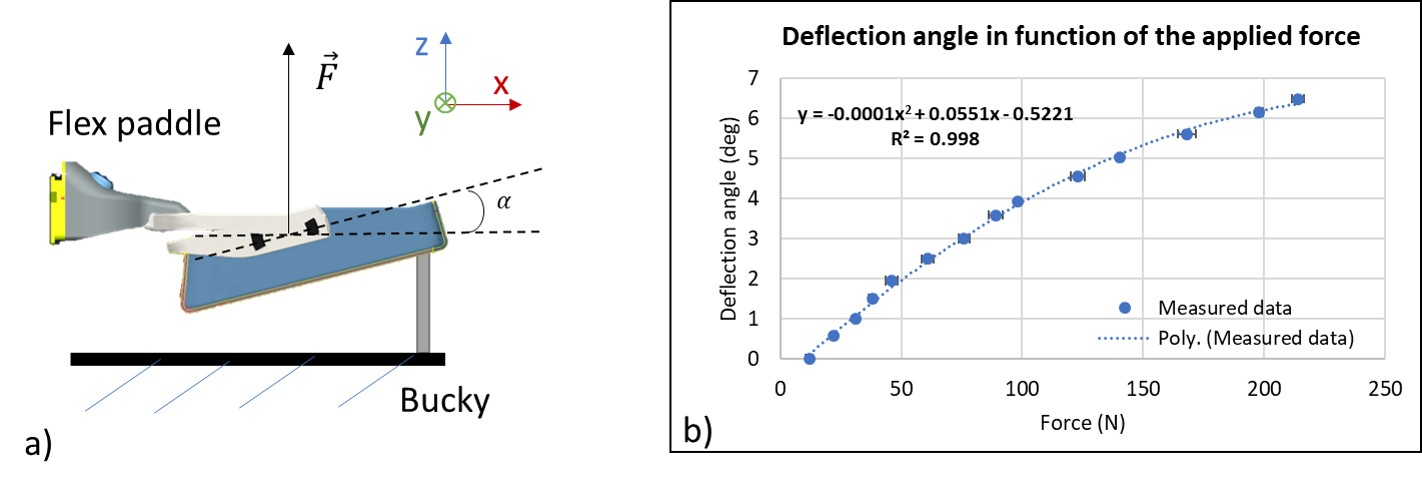
\includegraphics[width=0.9\textwidth,keepaspectratio]{figures/deflectionAngle.jpg} 
\caption{ a) Experiment set-up, b) Deflection angle as function of the applied force }\label{fig:deflectionangle}
\end{figure}

As concerns the third paddle model, namely the elastic paddle model (EPM\nomenclature{EPM}{Elastic Paddle Model}), the deflection due to the material properties was included. The paddle thickness was set to $4mm$ and it was made of Lexan material ($\lambda_{lexan}= 2250 \ MPa$ and $\nu_{lexan}= 0.4$).   Only one translational degree of freedom in the downward direction was considered. The paddle was modeled using shell elements. 

For the three paddle models, the interaction between the compression paddles and the breast was modeled using a frictionless contact. The penalty algorithm was used with a penetration factor equal to 0.1 and a contact stiffness equal to 1. 
 
\subsection{Breast compression mechanics}

The realism of breast compression simulations was verified by confrontation with real data. The compression of a small breast, like the one we have for the first volunteer, may be complex. Sometimes the technologist has to hold the breast between the image receptor and the paddle until the compression force is high enough to preclude the breast from sliding outside of the image receptor field of view. This difficulty is also present in a simulation framework, especially since we do not simulate the breast positioning gesture by the radiologist. To facilitate the compression process during the evaluation step, it was therefore decided to use only the larger breast geometry  provided by the second volunteer.

In a clinical framework, woman breasts are compressed in an up-right or prone body positions. Under compression, the gravity induced tissues pre-stresses can be neglected when compared to the compression-induced stresses \citep{han_development_2012, ruiter_model_based_2006, sturgeon_finite_element_2016}.  Therefore, the prone breast configuration was used as the reference configuration, neglecting the tissues internal pre-stresses due to gravity loading. The breast compression was simulated using the rigid and flex paddle models. 

Prior to breast compression simulations, the breast biomechanical model corresponding to the geometry of the second volunteer in prone configuration was developed. The optimization problem estimating the set of constitutive parameters is expensive in terms of the computation time.  Therefore, for this chapter, we decided to replace the tissues constitutive parameters of the second volunteer, with the ones found in the literature  \citep{han_nonlinear_2014,  rajagopal_modelling_2007, gefen_mechanics_2007}. The corresponding equivalent modulus for each involved tissue was chosen the following: $\lambda_{breast}=0.5 kPa$, $\lambda_{muscle}= 10kPa$, $\lambda_{skin}=10kPa$, $\lambda_{fascia}= 160kPa$.  Of course, with this assumption, this new biomechanical model does not properly represent the breast mechanics of the second volunteer.  However, it provides a realistic model with a larger breast volume and with stiffer breast tissue which may be used in a comparative study between various compression strategies.     

The cranio-caudal incidence was modeled by positioning the image receptor at the inframammary ligament level while the paddle compresses the breast by a downward movement. The compression was stopped when the target breast thickness was reached. Such target thickness was given by the data recorded during the most recent mammogram of the second volunteer (Table \ref{tab:forceandthichnessdata}). Figure \ref{fig:thicknessforcerelationNH} shows the breast thickness as function of the applied force for the flex and the rigid paddles. The breast thickness for the flex and the rigid paddles was considered constant. For a rigid paddle, the distance between the paddle and the image receptor was considered, named $h_r$  (Figure \ref{fig:thicknessforcerelationNH}). Concerning the flex paddle, distance between the image receptor and the paddle was measured at two distinct points, first at the nipple level (named $h_1$ in Figure \ref{fig:thicknessforcerelationNH}) and the second at the breast base (named $h_2$ in Figure \ref{fig:thicknessforcerelationNH}). Therefore, the breast thickness for the flex paddle (named $h_f$ on Figure \ref{fig:thicknessforcerelationNH}) is given by the mean value of $h_1$ and $h_2$. 
 
\begin{figure}[!h]
\centering
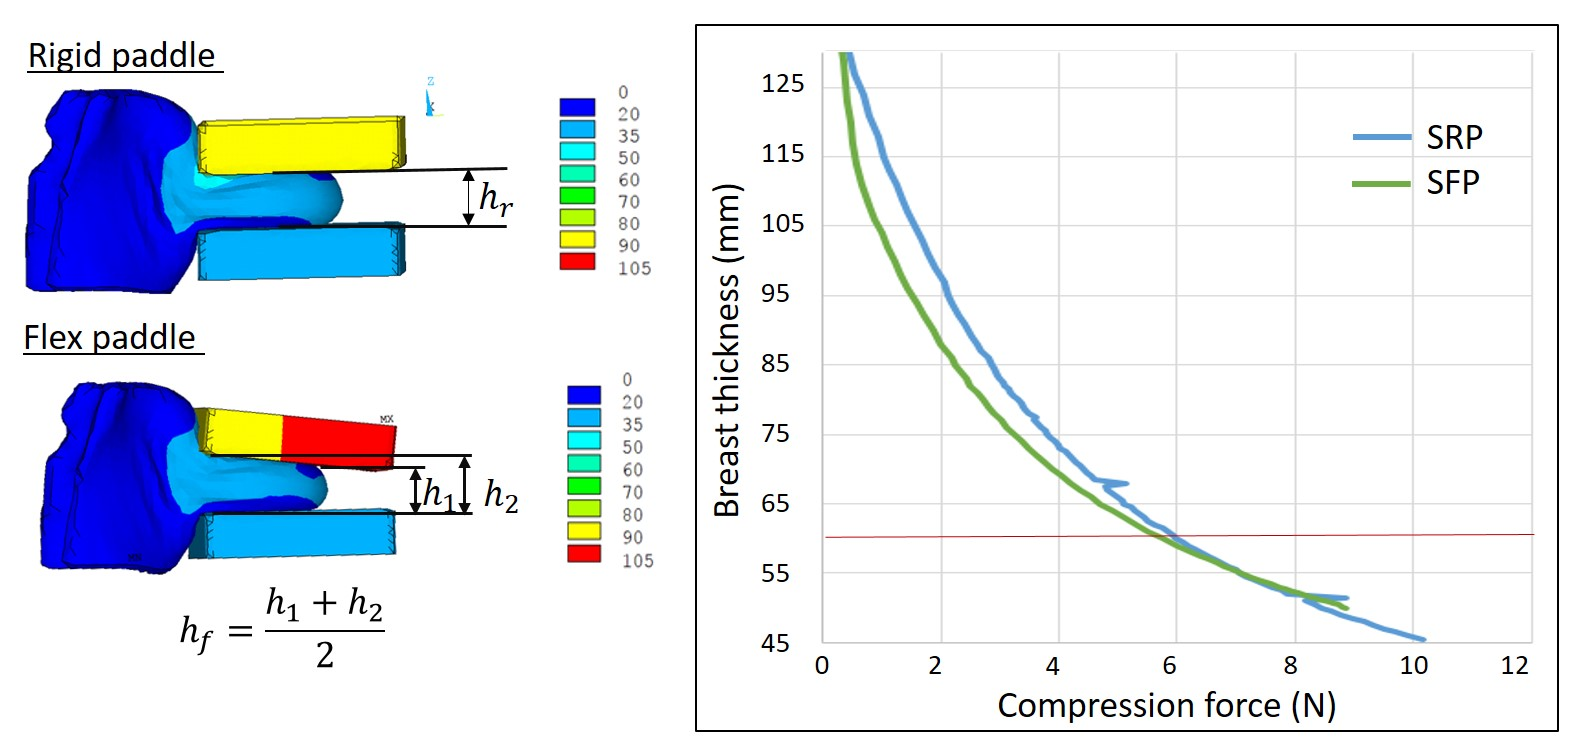
\includegraphics[width=0.9\textwidth,keepaspectratio]{figures/compressionforceNH.jpg} 
\caption{Breast flattening curve as function of the applied force for a Neo-Hookean strain energy function. SRP - standard rigid paddle, SFP -standard flex paddle}\label{fig:thicknessforcerelationNH}
\end{figure}

Several irregularities can be observed over the curve  describing the force-thickness relation when the breast is compressed with a rigid paddle, this numerical artifacts are due to inherent finite elements discretization errors.  One can see that, the total compression force at the target breast thickness ($50mm$) is about 15 times lower than the force measured during the volunteer's last mammography ($6N$ versus $94.8N$). Even if the chosen constitutive models were not accurately adapted to the patient mechanical properties, a force of $6N$ remains too low when compared to the standard compression force of $120N$ \citep{chida_reduced_2009}. Usually, a larger force is applied when compressing such large breast volumes as the one of the second volunteer.  Several compressions were tested (e.g. paddle closer to the juxtathoracic area, frictional contact with different friction coefficient) without observing any significant increase of the compression force. 

An analysis of the literature revealed that the constitutive parameters used to model breast compression are usually higher than the ones used to model the breast deformation under gravity loading. For example, Sturgeon G.M and colleagues \citep{sturgeon_finite_element_2016} have estimated the tissues deformation under compression considering the initial shear modulus for a Neo-Hookean strain energy function equal to $\mu_{skin} = 88kPa$, $\mu_{adipose} = 1kPa$ and $\mu_{glandular}= 10kPa$. Moreover, our simulations did not demonstrate the asymptotic behavior of the compression force versus breast thickness, as described by Groot J. et al. \citep{de_pain_2015}.  One can conclude that, for high strains, the soft tissues undergo a stiffening process more rapidly than the stiffening as described by a Neo-Hookean law.

The limitation of the Neo-Hookean model to capture the mechanical response of some nonlinear materials is well known \citep{kaliske_finite_1997}. For large strain rates, the Neo-Hookean material may undergo a relaxation and thus become easier to deform. Therefore, another strain energy model has to be considered for the modeling of breast compression.

\subsection{Gent strain energy function}
Giving that the Neo-Hookean strain energy function provide a poor estimation for large strains, the Gent strain energy function (see Section \ref{subsection:constitutivemodels}.a)  can be used as an alternative model. The Gent function is characterized by three parameters ($\mu$, $K$, and $J_m$). For small strains, it is resumed to the Neo-Hookean model \citep{chagnon_comparison_2004}. For large strains, the $J_m$ parameter acts as a stiffening parameter and defines the upper limit of the first invariant of the left Cauchy-Green deformation tensor (Figure \ref{fig:GentvsNeoStrain}.a).  When $J_m \longrightarrow \infty$, the Gent model is reduced to the Neo-Hookean model even for large strains (Figure \ref{fig:GentvsNeoStrain}.a).  
 
\begin{figure}[!h]
\centering
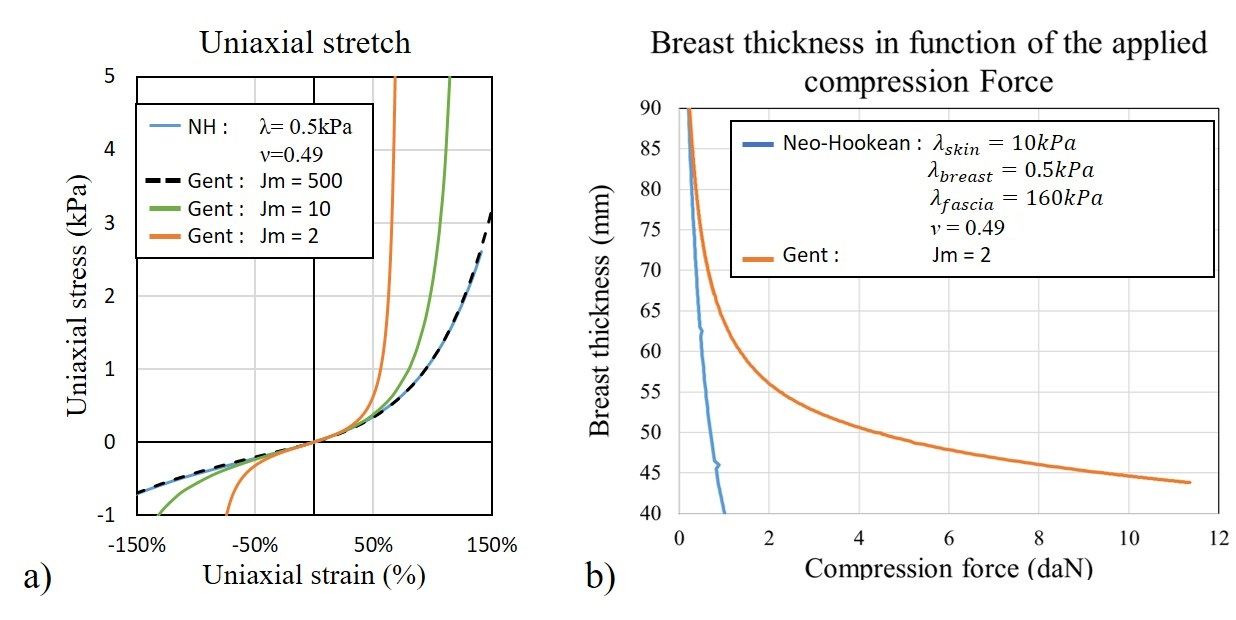
\includegraphics[width=1\textwidth,keepaspectratio]{figures/GentvsNeoStrain.jpg} 
\caption{a) Stress-strain relation for Neo-Hookean and Gent energy functions; b) Breast flattening curve as function of the applied force for a Gent energy function.}
\label{fig:GentvsNeoStrain}
\end{figure}

These properties are particularly interesting for our simulation framework. In chapter \ref{chapter:myBioMecaModel}, the material properties have been estimated and validated for multi-loading gravity simulations. Therefore, the tissues mechanical behavior is well estimated for relatively small strains. The strain range due to breast compression is significantly larger than the one due to gravity loading. In this respect, the $J_m$ parameter may be estimated such that, for relative small strains, the Gent model remains equivalent to the Neo-Hookean model. However for larger strains,  the energy function will behave asymptotically to approach a compression force equivalent to the standard compression force (Figure \ref{fig:GentvsNeoStrain}.b). Then, only the third parameter of the energy function has to be estimated ($J_m$), the initial shear modulus ($\mu$) and the Bulk modulus ($K$) being already known from the multi-loading gravity optimization process.

Figure \ref{fig:GentvsNeoStrain}.b shows the breast flattening curve as function of the applied force when using Neo-Hookean and Gent material models. One can see that, when using the Gent model the curve shape is closer to the results described by Groot J.E. and colleagues \citep{de_pain_2015} from experimental data on real patients. Moreover, for a breast thickness of $45 \ mm$, the compression force obtained with the Gent material model is 10 times higher than the one obtained with the Neo-Hookean material model, i.e. $10 \ N$ versus $100 \ N$ (Figure \ref{fig:GentvsNeoStrain}). The Gent model definitively provides more realistic simulation results. Therefore, in the next section, the constitutive parameters of the Gent function will be estimated in order to improve breast compression mechanical behavior for both breast models. 


\subsection{Updated material constitutive models}
We have seen that a Neo-Hookean model can not describe correctly the breast mechanics under compression. The force needed to flatten the breast during simulation was too small when compared to the mean compression force measured in mammography. 
The Gent model showed to perform better, giving a more realistic breast flattening curve as function of the applied force (Figure \ref{fig:GentvsNeoStrain}). Therefore, to compute tissue deformations under compression, the Gent energy function was used. 

For the following, the compression simulations were performed on the right breast only. The constitutive parameters for the Gent energy strain function were chosen as follows. For the first volunteer the tissues mechanical properties have already been estimated. Therefore the equivalent Young's modulus of each tissue was kept as defined by the multi-loading gravity simulations ($\lambda_{breast}^r=0.3 kPa$, $\lambda_{muscle}= 10kPa$, $\lambda_{skin}=4 kPa$, $\lambda_{fascia}=120 kPa$). For the second volunteer, the constitutive parameters are unknown. However, in order to build up a new mechanical behavior, different from the first volunteer, the equivalent Young's modulus as described in the literature can be used. The appropriate values were selected among studies which have provided an in-vivo parameters estimation within similar frameworks  ($\lambda_{breast}^r=0.5 kPa$, $\lambda_{muscle}= 10kPa$, $\lambda_{skin}=10kPa$, $\lambda_{fascia}= 160kPa$) \citep{han_nonlinear_2014, rajagopal_modelling_2007, gefen_mechanics_2007}. Therefore, the second model represents larger breast volume with stiffer tissues.  

To estimate the $J_m$ parameter, additional information was needed. To this end, the subjects were asked to provide the data from their most recent mammogram. Several compression simulations were performed to estimate the $J_m$ value that gives the compression force and the breast thickness as measured during the mammography ( Table \ref{tab:forceandthichnessdata}). The Poison ratio for these simulations was changed to $0.499$ (nearly incompressible material allowing a better convergence of the simulations). According to the sensitivity analysis performed in Chapter \ref{chapter:myBioMecaModel}, this change does not significantly impact the mechanics of the small breast volume in the multi-loading gravity framework. For the first volunteer, a breast thickness of $46mm$ with a compression force of $22N$ is obtained with  $J_m = 1$. For the second volunteer, a breast thickness of $48mm$ with a compression force of $95N$ is obtained with $J_m = 2$. 

Figure \ref{fig:forceThicknessResults} shows the breast flattening curve as function of the applied force obtained with rigid and flex paddle models. All simulations were performed with the Gent strain energy function. 

\begin{figure}[!h]
\centering
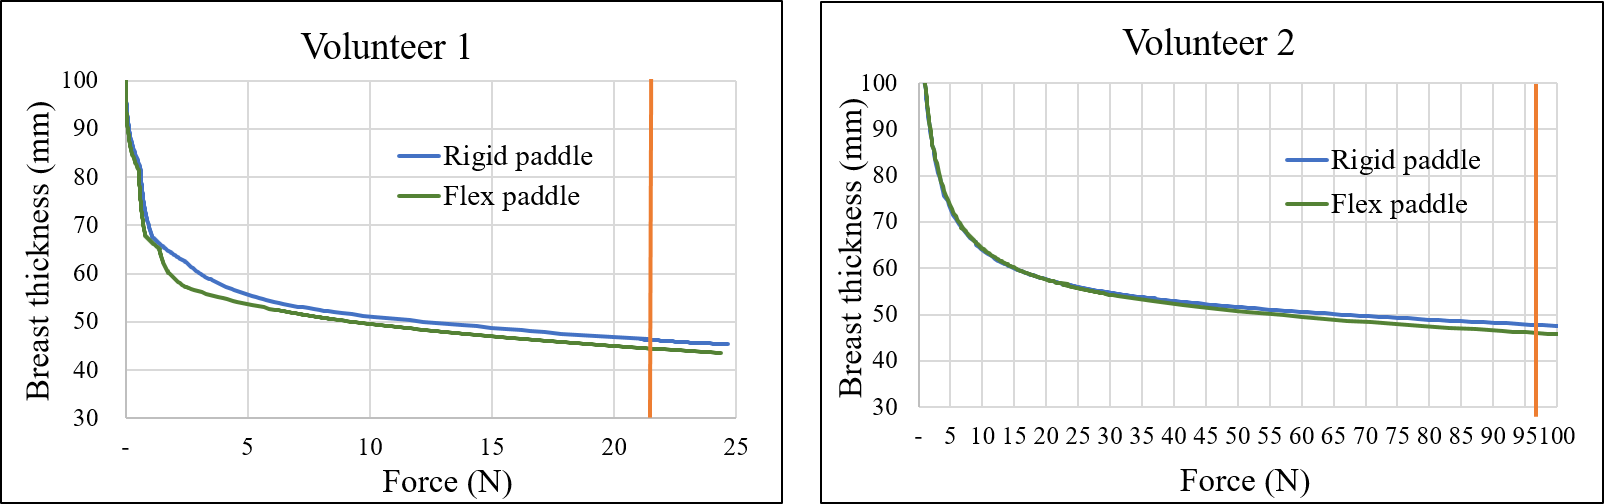
\includegraphics[width=1\textwidth,keepaspectratio]{figures/forceThicknessResults.png} 
\caption{Resulting breast flattening curve as function of the compression force with Gent constitutive model. }\label{fig:forceThicknessResults}
\end{figure}
    
 One can see that the compression force range is comparable with the one measured during mammography. Moreover, the curve behavior is similar with the one given by Groot J.E. et al \citep{de_pain_2015}, with an asymptotic behavior at the end of breast compression.
 
 In this section, it was assumed that introducing a Gent strain energy function will have a non-significant impact on breast mechanics under gravity loading since the Neo-Hookean and the Gent models have similar behaviors for small deformations. Therefore we can consider that the previous optimization process performed on the breast volume of the first volunteer remains valid. 
 
 \subsection{ Gent model and breast mechanics under gravity loading}
 
 When looking back to the Gent function properties, an appropriate  $J_m$ parameter was defined as following. The $J_m$ value has to be small enough in order to obtain an appropriate compression force. And in the same time, it has to be high enough in order to preserve the model fidelity to the gravity loading deformations.
 
 In Chapter \ref{chapter:myBioMecaModel}, the biomechanical breast model corresponding to the first volunteer was evaluated for Neo-Hookean material models. The worst estimate was found in supine tilted configuration due to the tissues over sliding on the lateral direction (maximal distance of $26.03 \ mm$). Introducing Gent tissues model should not impact the breast deformation under gravity loading. However, when looking at the supine tilted configuration simulated with Neo-Hookean material, large deformations were observed at the fascia and skin surfaces. Figure \ref{fig:strain_range_neo} shows the strain rates in supine, prone and supine tilted configurations obtained with Neo-Hookean material models. The strain rates over the skin and fascia surfaces in supine tilted configuration were twice larger than ones observed in supine and prone breast configurations. Therefore, considering the Gent model in the multi-loading gravity simulations may improve the supine tilted estimate by reducing the fascia and skin deformations under large strain. 


\begin{figure}[!h]
\centering
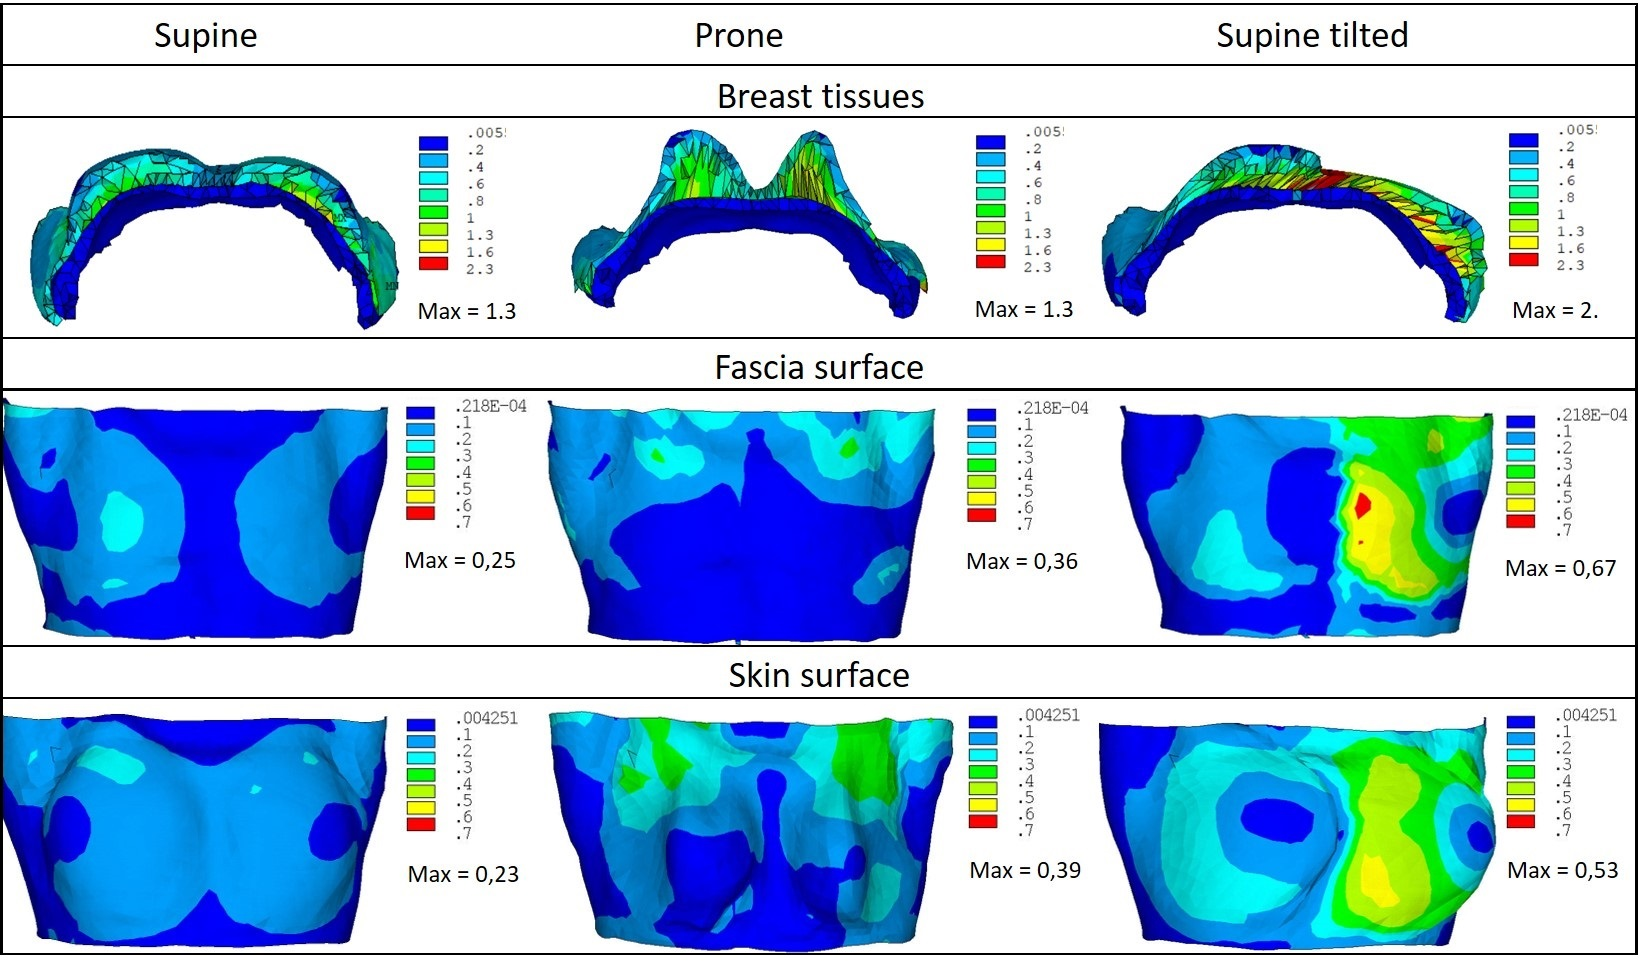
\includegraphics[width=\textwidth,keepaspectratio]{figures/strain_range_neo.jpg} 
\caption{Strain range distribution when using a Neo-Hookean material model. }\label{fig:strain_range_neo}
\end{figure}
 

\begin{figure}[!h]
\centering
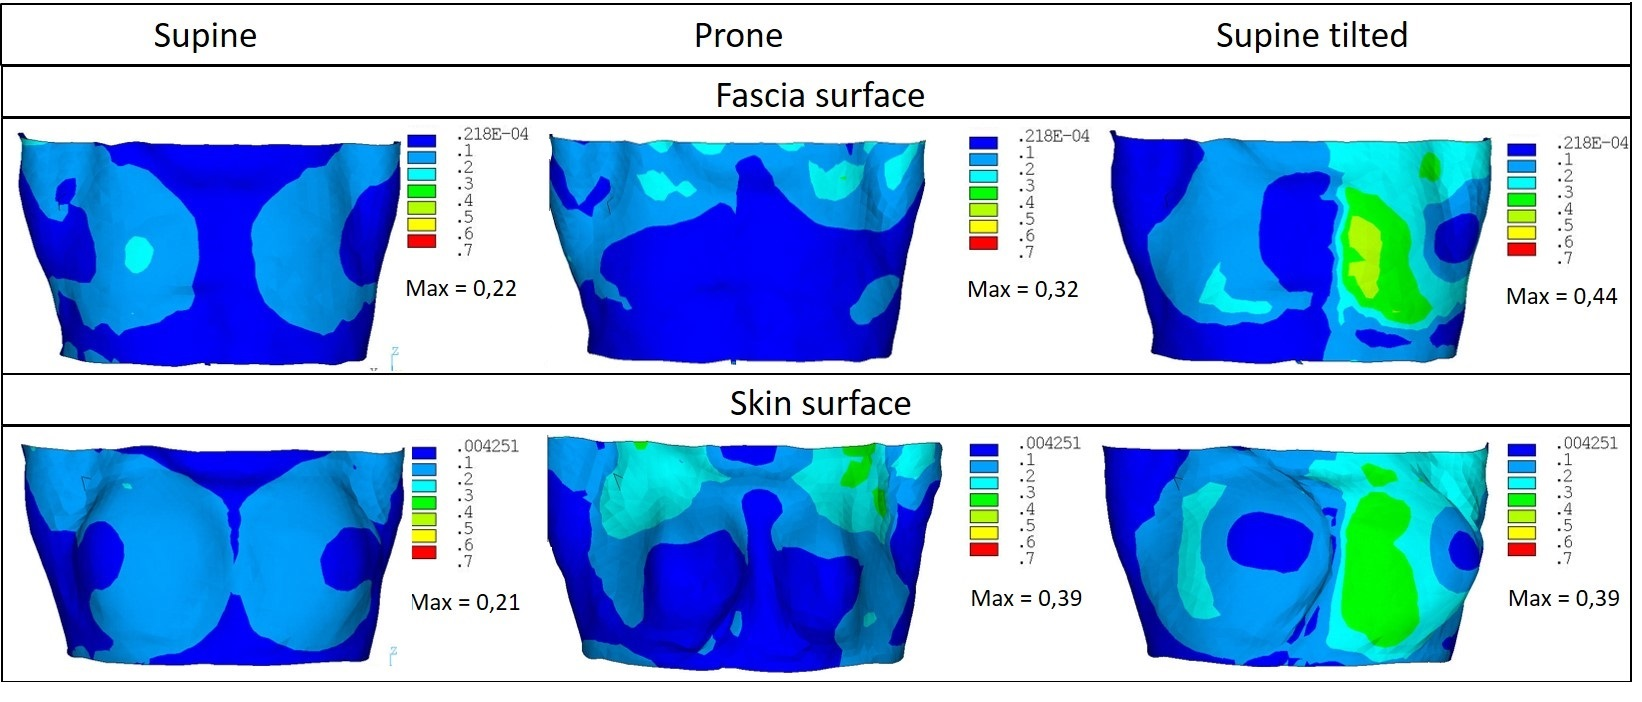
\includegraphics[width=\textwidth,keepaspectratio]{figures/strain_range_gent.jpg} 
\caption{Strain range distribution when using a Gent material model. }\label{fig:strain_range_gent}
\end{figure}

 Several simulations were performed considering $J_m = 1$, as identified during the compression simulations. However this value seems to constrain too much the tissues deformation in prone and supine configurations. It will be shown that the compression force is highly dependent on the paddle positioning with respect to the chest wall (Section \ref{subsection:breastpositioning}). For an accurate estimation of the parameter $J_m$, more data is needed concerning the paddle position during compression. In our study, the paddle position with respect to the chest wall was not available. Therefore, the estimated $J_m$ value is only an approximation and does not characterize completely the subject breast mechanics.    
 
When the multi-loading gravity simulations were performed using a Gent model with $J_m=2$, better estimates were obtained. In this respect, to show the impact of using a Gent model within multy-loading gravity simulations, the parameter $J_m$ of all involved tissues was set to 2. Figure \ref{fig:strain_range_gent} shows the corresponding strain range distributions over the skin and fascia surfaces.  The maximal strain does not change significantly in supine and prone configurations ( less than $10\%$ of difference). On the other hand, important changes were observed over the left breast in supine tilted configuration. The maximal strain range decreased by about $30\%$ over the fascia surface and by about $26 \ \%$ over the skin surface. As previously described, these tissues provide the breast support, accordingly,  the lateral displacement of the left breast was reduced.

 The estimates of breast external geometry in the three configurations computed using the Gent material models are presented in Figure \ref{fig:modelevaluation_gent}. One may see that the breast deformations in supine and prone configurations remain on the same range of precision. The Hausdorff distance being increased by only $0.46 \ mm$ and $0.6\ mm$ respectively (maximal distance by $0.17$ and $0.93 \ mm$ respectively). Contrariwise, the sliding of the left breast was significantly reduced. Even if the Hausdorff distance was reduced by only $1 \ mm $ ($5.15 \ mm$ with Gent models versus $6.14 \ $ with Neo-Hookean models), an significant decrease of $10 \ mm$ in maximal distance  was observed. Moreover, smaller deformations imply also better solution convergence. 
   

\begin{figure}[!h]
\centering
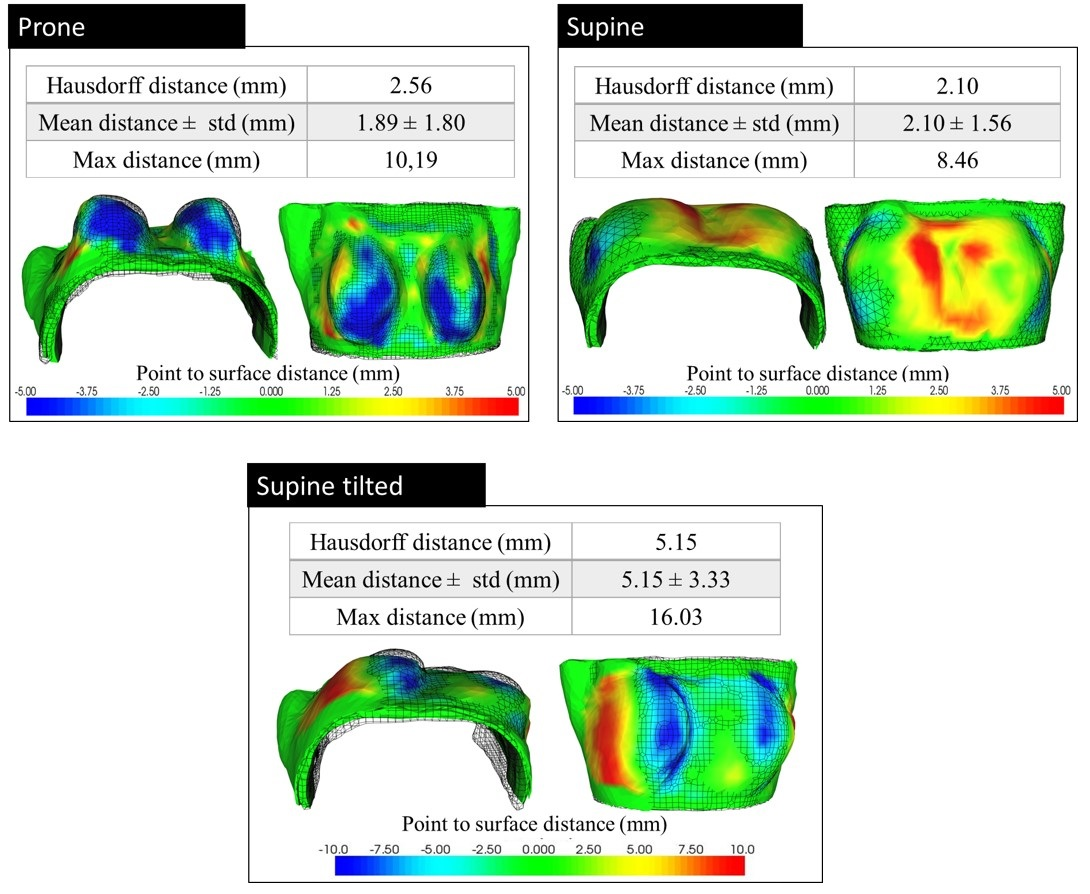
\includegraphics[width=\textwidth,keepaspectratio]{figures/modelevaluation_gent.jpg} 
\caption{Difference between estimated and measured breast surfaces, in supine, prone and supine tilted configurations obtained with a Gent material model. }\label{fig:modelevaluation_gent}
\end{figure}

Using the Gent model improved the overall performance of the breast biomechanical model. However, different values of  parameter $J_m$ were used to simulate breast deformations under compression and under gravity loading. A more detailed study is needed to find appropriate constitutive parameters characterizing a wider panel of breast deformations.  

 In this chapter we assumed a constant value of $J_m$ for all involved hyperelastic material models, yet their mechanical response under large stresses are different. A variable $J_m$ parameter within tissues types may improve model accuracy.  On the other hand, it also implies an optimization process with more constitutive parameters. An optimization process with a higher number of variables is also more expensive in terms of data and time resources. 
 
 For the breast compression simulations presented below the parameter $J_m$ for the first volunteer was set to 1. This assumption satisfies the thickness-force  relation obtained during the mammography exam.

\section{Simulation of digital images }
Once the compression simulations were performed, the compressed breast geometry was extracted and used to create numerical object defined by the means of a surface meshes, also named numerical phantoms. These objects were used as input for the CatSim environment able to simulate a digital mammography  acquisition \citep{de_low_2014,de_catsim_2007}. The simulated images were used to assess the image quality as function of the compression paddle design.

\subsection{Physical characteristics}
The X-ray projections of phantom objects were simulated using a GE Senographe Pristina system topology (Figure \ref{fig:systemgeometry}). The focal spot was modeled as a point source. A $24\ keV$ mono-energetic X-ray beam was considered.  This beam quality is similar to the effective X-ray energy of a $34\ kVp$ Rh/Ag target/filter spectrum filtered by a $46\ mm$ compressed breast. Spreading of the light photons in the CsI scintillator of the detector was modeled by filtering the detected X-ray beam by an empirically assessed modulation transfer function of the cesium iodide (CsI) scintillator. X-ray scatter from the test object and other system components were not included in the simulation. Only quantum noise, modelled by a Poison random distribution, was considered as noise source. The simulated X-ray flux was tuned to match the average signal intensity ($\langle SI \rangle$) and signal-to-noise ratio (SNR) measured in real images of a $46\ mm$ thick, $20\%$ fibroglandular equivalent phantom acquired with the automatic exposure control. To do so, a calibration was performed on a real Senographe Pristina mammography unit.


\begin{figure}[!h]
\centering
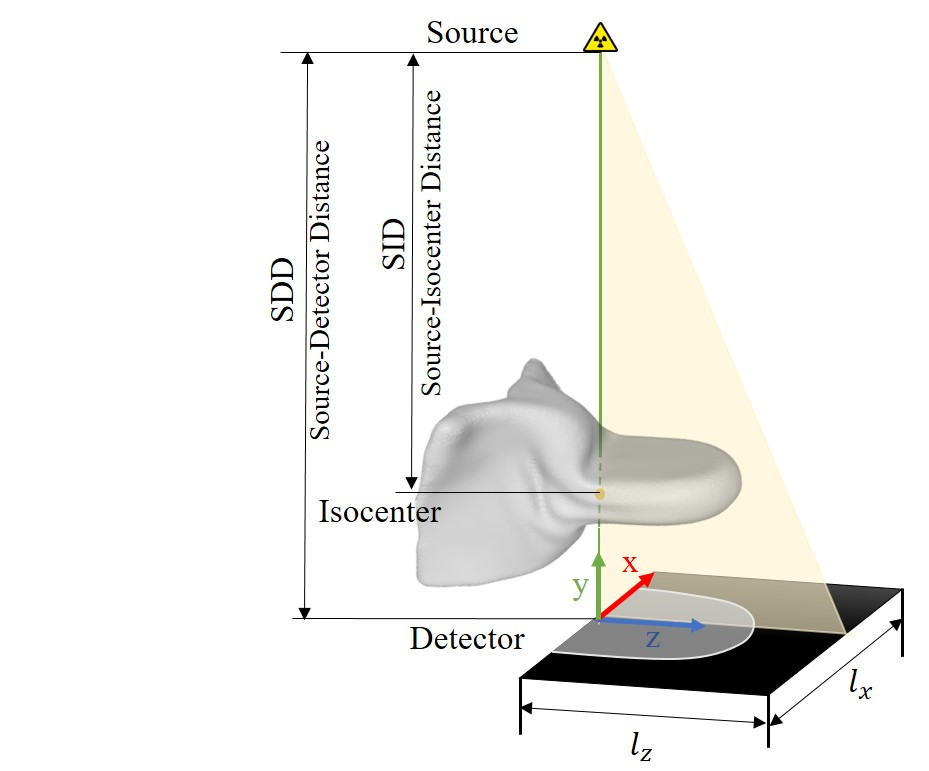
\includegraphics[width=0.65\textwidth,keepaspectratio]{figures/systemgeometry.jpg} 
\caption{A schematic illustration og the simulated GE Senographe Pristina TM mammography unit.}
\label{fig:systemgeometry}
\end{figure}
%SDD = 660mm, SID = 636.76 

\subsection{Breast phantom objects}

The phantoms were created by first extracting the compressed breast external shape. Then, a set of virtual microcalcifications ($\mu calc$) were inserted into each compressed breast volume. The smallest breast volume contains 21 microcalcifications arranged in a matrix of 7 rows and 3 columns (Figure \ref{fig:microcalcifications}.a). The largest breast volume contains 56 microcalcifications arranged in a matrix of 7 rows and 8 columns. The matrix of $\mu calc$ was parallel with the entrance surface of the image receptor and was positioned at the breast mid thickness (Figure \ref{fig:microcalcifications}.b). The distance between two consecutive columns or rows was equal to $10\ mm$. The anatomical background was assumed to be a uniform breast-equivalent material composed of glandular/adipose tissue with a $20/80$ ratio. Two simulations were performed for each compression considering microcalcifications of $0.2\ mm$ and $0.3\ mm$ in diameter.

\begin{figure}[!h]
\centering
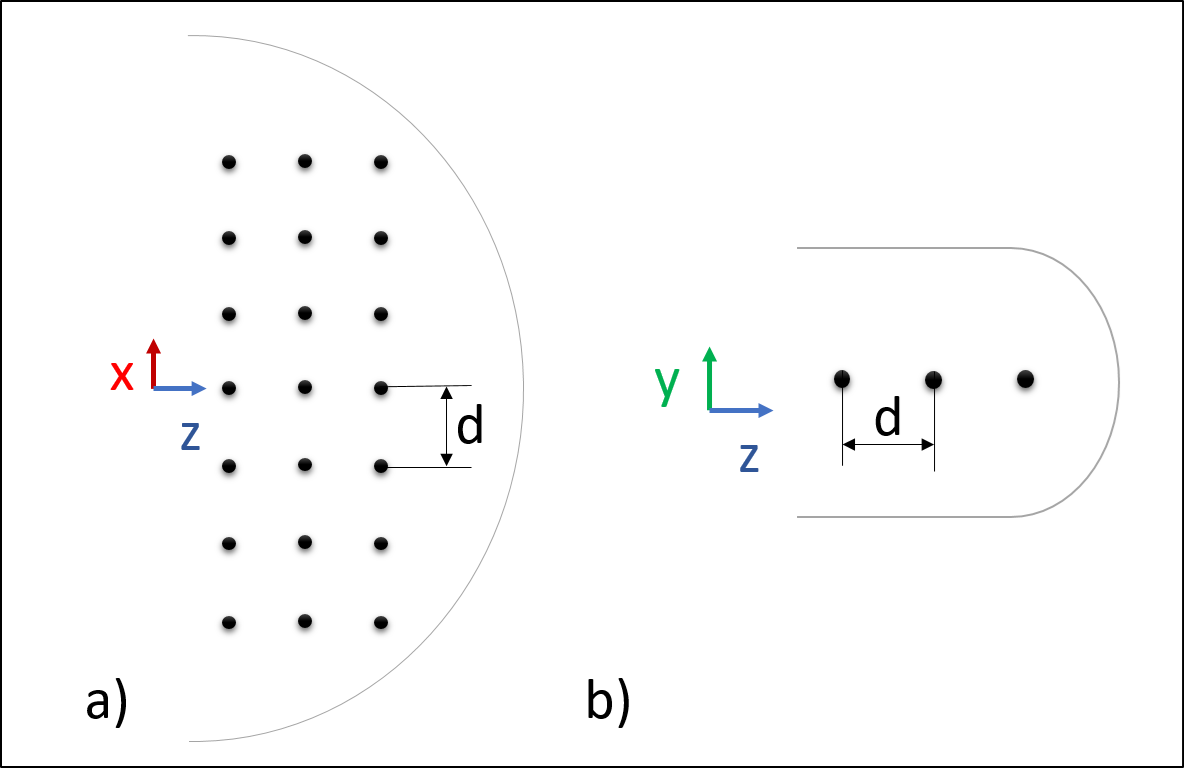
\includegraphics[width=0.5\textwidth,keepaspectratio]{figures/microcalcifications.png} 
\caption{Microcalcification distribution over the smallest breast volume $(d=10mm)$: a) axial view, b) sagittal view.}\label{fig:microcalcifications}
\end{figure}


Microcalcifications were simulated as round-shaped surface mesh. To add irregularities, initially spherical objects were randomly deformed. Their X-ray attenuation properties were chosen to correspond with the attenuation of aluminium (Al) at $24 \ keV$, their volumetric mass density correspond to $60\%$ of the Al density (i.e. $1.63\ \frac{kg}{m^3}$).  The choice of $24\ keV$ corresponds to the photon energy of the x-ray source used in our study. 


\section{Compression quality metrics}\label{section:compressionqualitymetrics}

The measures used to quantify the three criteria characterizing the quality of breast compression (patient comfort, image quality and average glandular dose) are described in the following section.  

\subsection{Patient comfort}

Today, pain estimation and quantification still remain an open question. The perceived pain during mammography, or its interpretation, may depend on the social status, pain history or psychological condition of the patient. But it also depends on physical parameters such as compression force, amount of strain or pressure at skin surface. In clinical studies, the patient comfort is assessed using pain scales. The repeatability of such methods is questionable, because they are based on the patient own interpretation and expertise. More quantitative measures such as pupil dilatation or heart beat rate are interesting in assessing the patient comfort; however they may indicate not only the pain but also the fear of pain.        

In this work, only physical pain associated with tissues deformations was considered. In this scope, the maximal strain and stress intensities as well as the maximal pressure intensity at the contact surface were chosen as pain quantifiers. Their distribution over the breast volume were obtained from FE simulations of breast compression and were analysed in order to compare the patient experience between two distinct compression systems. 

\subsection{Image quality }\label{section:averagegalndulardose}
 To assess image quality, the signal-difference-to noise ratio (SDNR\nomenclature{SDNR}{Signal Difference to Noise Ratio})  and the signal-to-noise ratio (SNR\nomenclature{SNR}{Signal to Noise Ratio})  were measured in the raw simulated images. To this end, squared ROIs of  $1cm \times 1cm$ were defined centered on the $\mu calcs$ position. The pixels inside of each ROI were divided into two sets. Pixels located  at the ROI's center within a radius equal to the radius of the $\mu calcs$  represented the $\mu calcs$ attenuated signal intensity ($SI_{\mu calc}$). Pixels located within the ROI but outside the $\mu calc$ radius represent the background signal intensity ($SI_{back}$). The two sets were used to compute the average detected signal per $\mu calcs$ pixel ($\langle SI_{\mu calc}\rangle$), the average detected signal per background pixel  ($\langle SI_{back}\rangle$) and the standard deviation in the background signal intensity $\sigma_{back}$:
 \begin{align}
 \langle SI_{\mu calc}\rangle& = \frac{1}{\vert SI_{\mu calc}\vert} \sum_{p_i \in SI_{\mu calc}}p_i \\
  \langle SI_{back}\rangle &= \frac{1}{\vert SI_{back}\vert} \sum_{p_i \in SI_{back}}p_i\\
  \sigma_{back} &= \sqrt{\frac{1}{\vert SI_{back}\vert} \sum_{p_i \in SI_{back}} (p_i- \langle SI_{back}\rangle)^2}
  \end{align}
Where $\vert\cdot\vert$  is the number of pixels in the respective set.

  The SDNR per pixel of the inserted microcalcifications is defined as follows
 \begin{equation}
 SDNR = \frac{\langle SI_{back}\rangle - \langle SI_{\mu calc}\rangle}{\sigma_{back}},
\end{equation}

 
The SNR per background pixel was defined as follows  
 \begin{equation}
 SNR = \frac{\langle SI_{back}\rangle}{\sigma_{back}}.
\end{equation}



\subsection{Average glandular dose}
The estimation of the dose delivered to the glandular tissue remains an essential component of quality control in X-ray mammography. We derived the average glandular dose using the approach proposed by Dance D. \citep{dance_additional_2000} regardless the paddle type. The method uses conversion factors to relate measurements of the incident air kerma $K$ at the upper surface of the breast to the mean dose absorbed by the breast glandular tissue. 

\begin{equation}
AGD = K g c s
\end{equation}

Where g and s are conversion factors giving the AGD in function of the target/filter combination and the breast thickness (range between $20$ and $110\ mm$) for a breast glandularity of $50\%$. The factor c extends the AGD estimation for different breast glandularity. Monte-Carlo simulation was used to estimate these factors by modeling the compressed breast as a semi-circular cross section cylinder. 

The numerical phantom was characterized by a uniform thickness, while mammography compression implies variable breast thickness due to paddle elasticity (SRP) and paddle flexibility (SFP). In a clinical framework, the breast thickness is adjusted by applying an offset characterizing the paddle deflection during compression.      

For the rigid paddle model, as paddle elasticity was neglected, the AGD was computed assuming the breast thickness is equal to the distance between the image receptor and the paddle itself. Regarding the flex paddle, the breast thickness decreases quasi-linearly from the chest wall to the nipple. Thus, breast thickness was computed as the mean of the maximal and minimal distance over the breast contact area.

\section{Results}\label{section:breastcompressionevaluation}
Two studies were performed using the previously defined components for modeling the breast compression and simulating digital mammography. First, the results of a comparative study between flex and rigid paddles is presented with the effects on image quality, AGD and patient comfort. Then, the impact of paddle positioning on breast mechanics is analysed.   
\subsection{Compression quality for rigid and flex paddles}

To compare the breast compression quality when using a standard rigid paddle against a standard flex paddle, the rigid and flex paddle models were used. The right breasts of the two volunteers were first compressed until the target breast thickness measured during mammography was obtained (Table \ref{tab:forceandthichnessdata}). Then, the breast phantoms with $\mu calc $ were imported into CatSim environment and mammography images were simulated. The compression quality were measured in terms of image quality, average glandular dose and patient comfort.

The resulting breast thickness after compression varies by less than $2mm$ between rigid and flex paddles for both volunteers (Table \ref{fig:table_compression_results}). Accordingly, no significant difference was found between the estimated AGD, while dose reductions of $2.6 \%$ for the smaller breast and $4.2\%$ for the larger breast were observed in favor of the flex paddle.

\begin{figure}[!h]x-ray
\centering
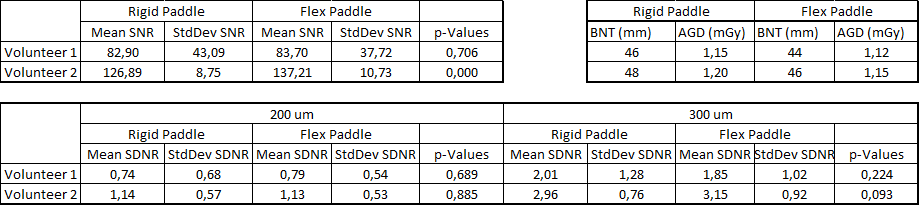
\includegraphics[width=\textwidth,keepaspectratio]{figures/table_compression_results.png} 
\caption{Breast nominal thickness (BNT), average glandular dose (AGD), signal-to-noise-ratio (SNR) and signal-difference-to-noise (SDNR) for both volunteers and both compression paddle types}\label{fig:table_compression_results}
\end{figure}

The SNR and SDNR have been estimated and compared between flex and rigid paddles. When using a flex paddle instead of a rigid paddle on the largest breast (volunteer 2), we observe a statistically significant higher SNR. We do not observe statistically significant differences on SDNR for both $200\mu m$ and $300\mu m$ microcalcifications, when using rigid or flex paddle. Therefore, despite a breast thickness varying linearly from chest wall to nipple when the flex compression paddle is used, the image quality is preserved or improved compared to the image quality obtained with the rigid compression paddle.

In a clinical study, Broeders M.J. et al. \citep{broeders_comparison_2015} have also compared the image quality and patient comfort between the standard rigid and flex paddles. According to the authors, the standard flex paddle performed slightly better image quality in the projected breast area, however it moved breast tissue from the image area at chest wall side. According to our compression simulation, for the small breast volume, no difference in tissues lateral displacement was observed. On the other hand, for the larger breast, using the flex paddle has indeed increased the tissues displacement toward the chest wall side , but not by more than $4 \ mm$ (Figure \ref{fig:rigid_flex_y_displacement}).  

\begin{figure}[!h]
\centering
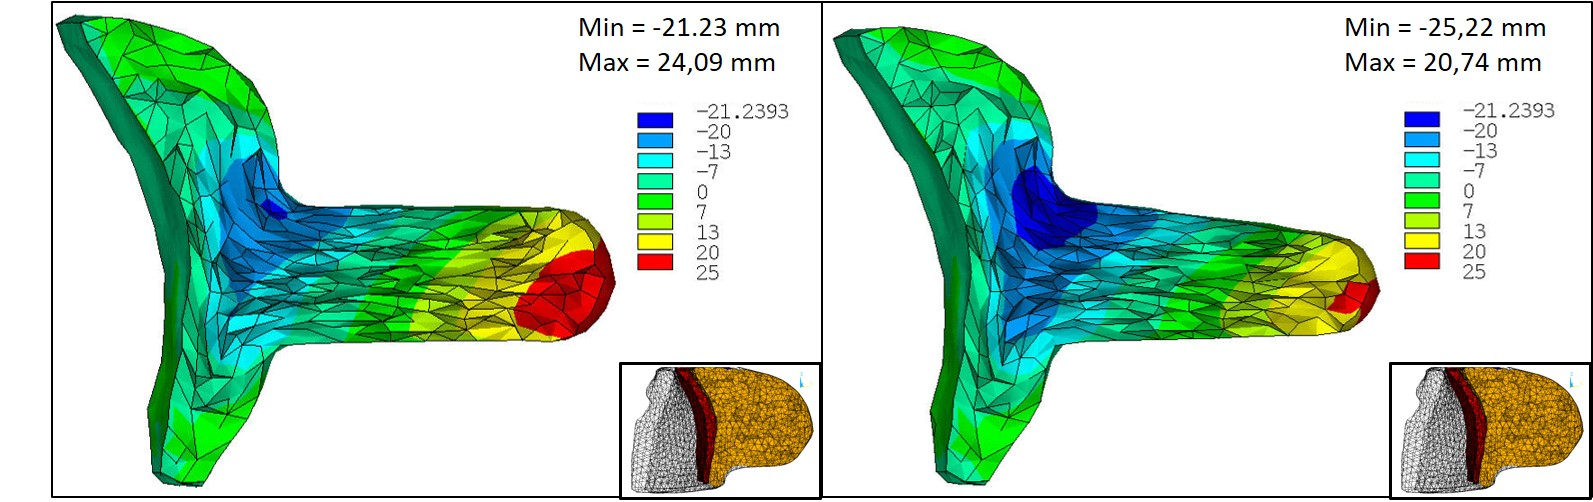
\includegraphics[width=1\textwidth,keepaspectratio]{figures/rigid_flex_y_displacement.jpg} 
\caption{Node displacements on the direction parallel to the paddle (Oy axis).}\label{fig:rigid_flex_y_displacement}
\end{figure}

To assess the patient comfort during compression, the resulting internal stress and strain distributions, as well as the contact pressure maps were derived. These data were collected at compressive forces of 22 N for the first volunteer (Figure \ref{fig:subject1_compressionResults}) and 95 N for the second one (Figure \ref{fig:subject2_compressionResults}).

\begin{figure}[h!]
\centering
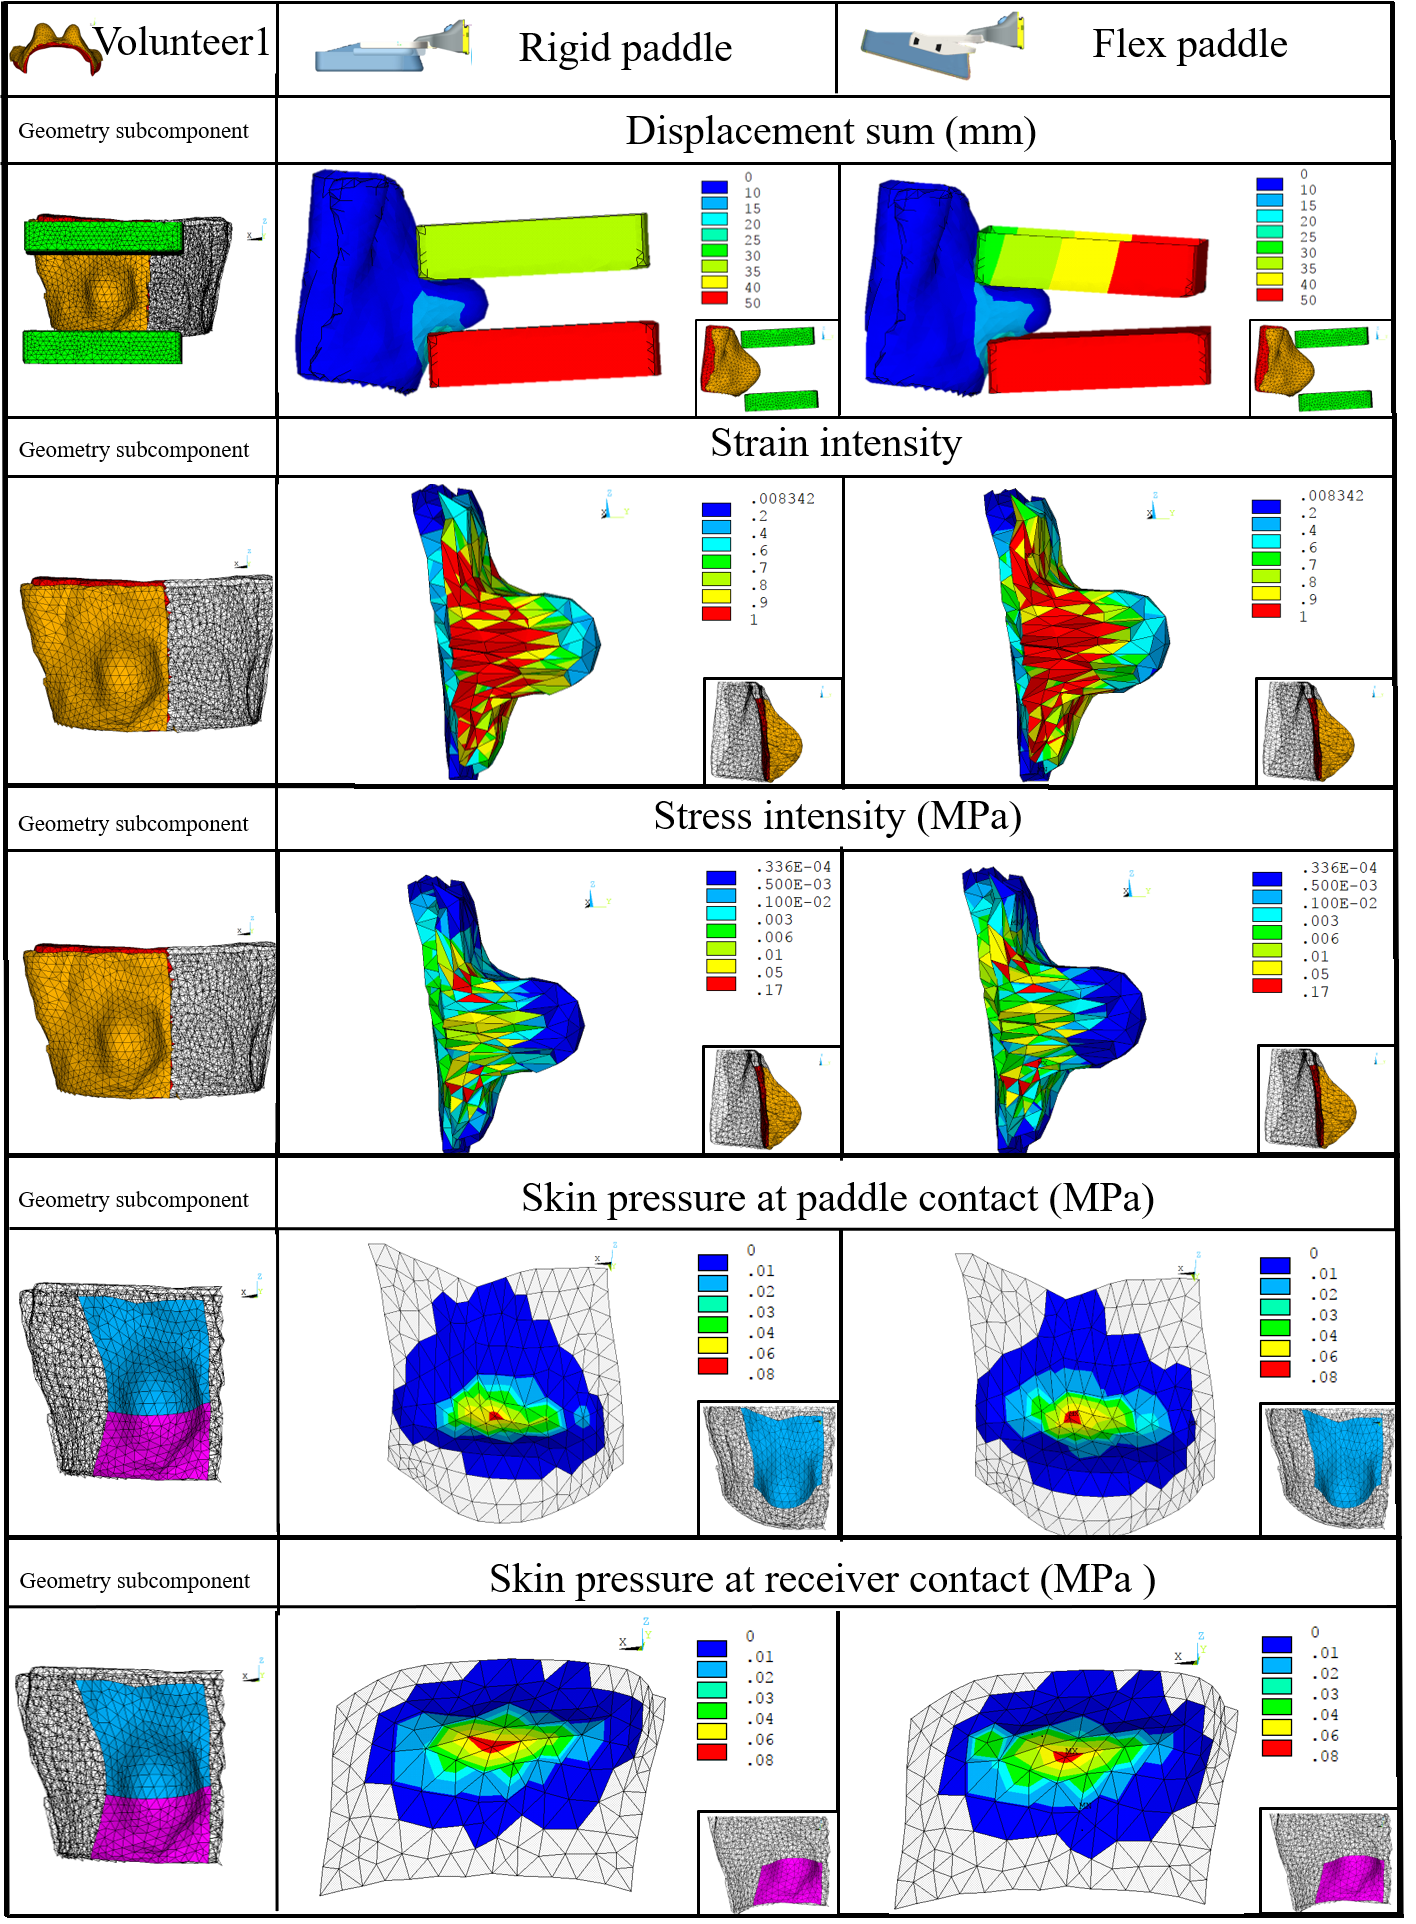
\includegraphics[width=0.9\textwidth,keepaspectratio]{figures/subject1_compressionResults.png} 
\caption{Stress, strain and contact pressure distribution for the first volunteer}\label{fig:subject1_compressionResults}
\end{figure}

\begin{figure}[h!]
\centering
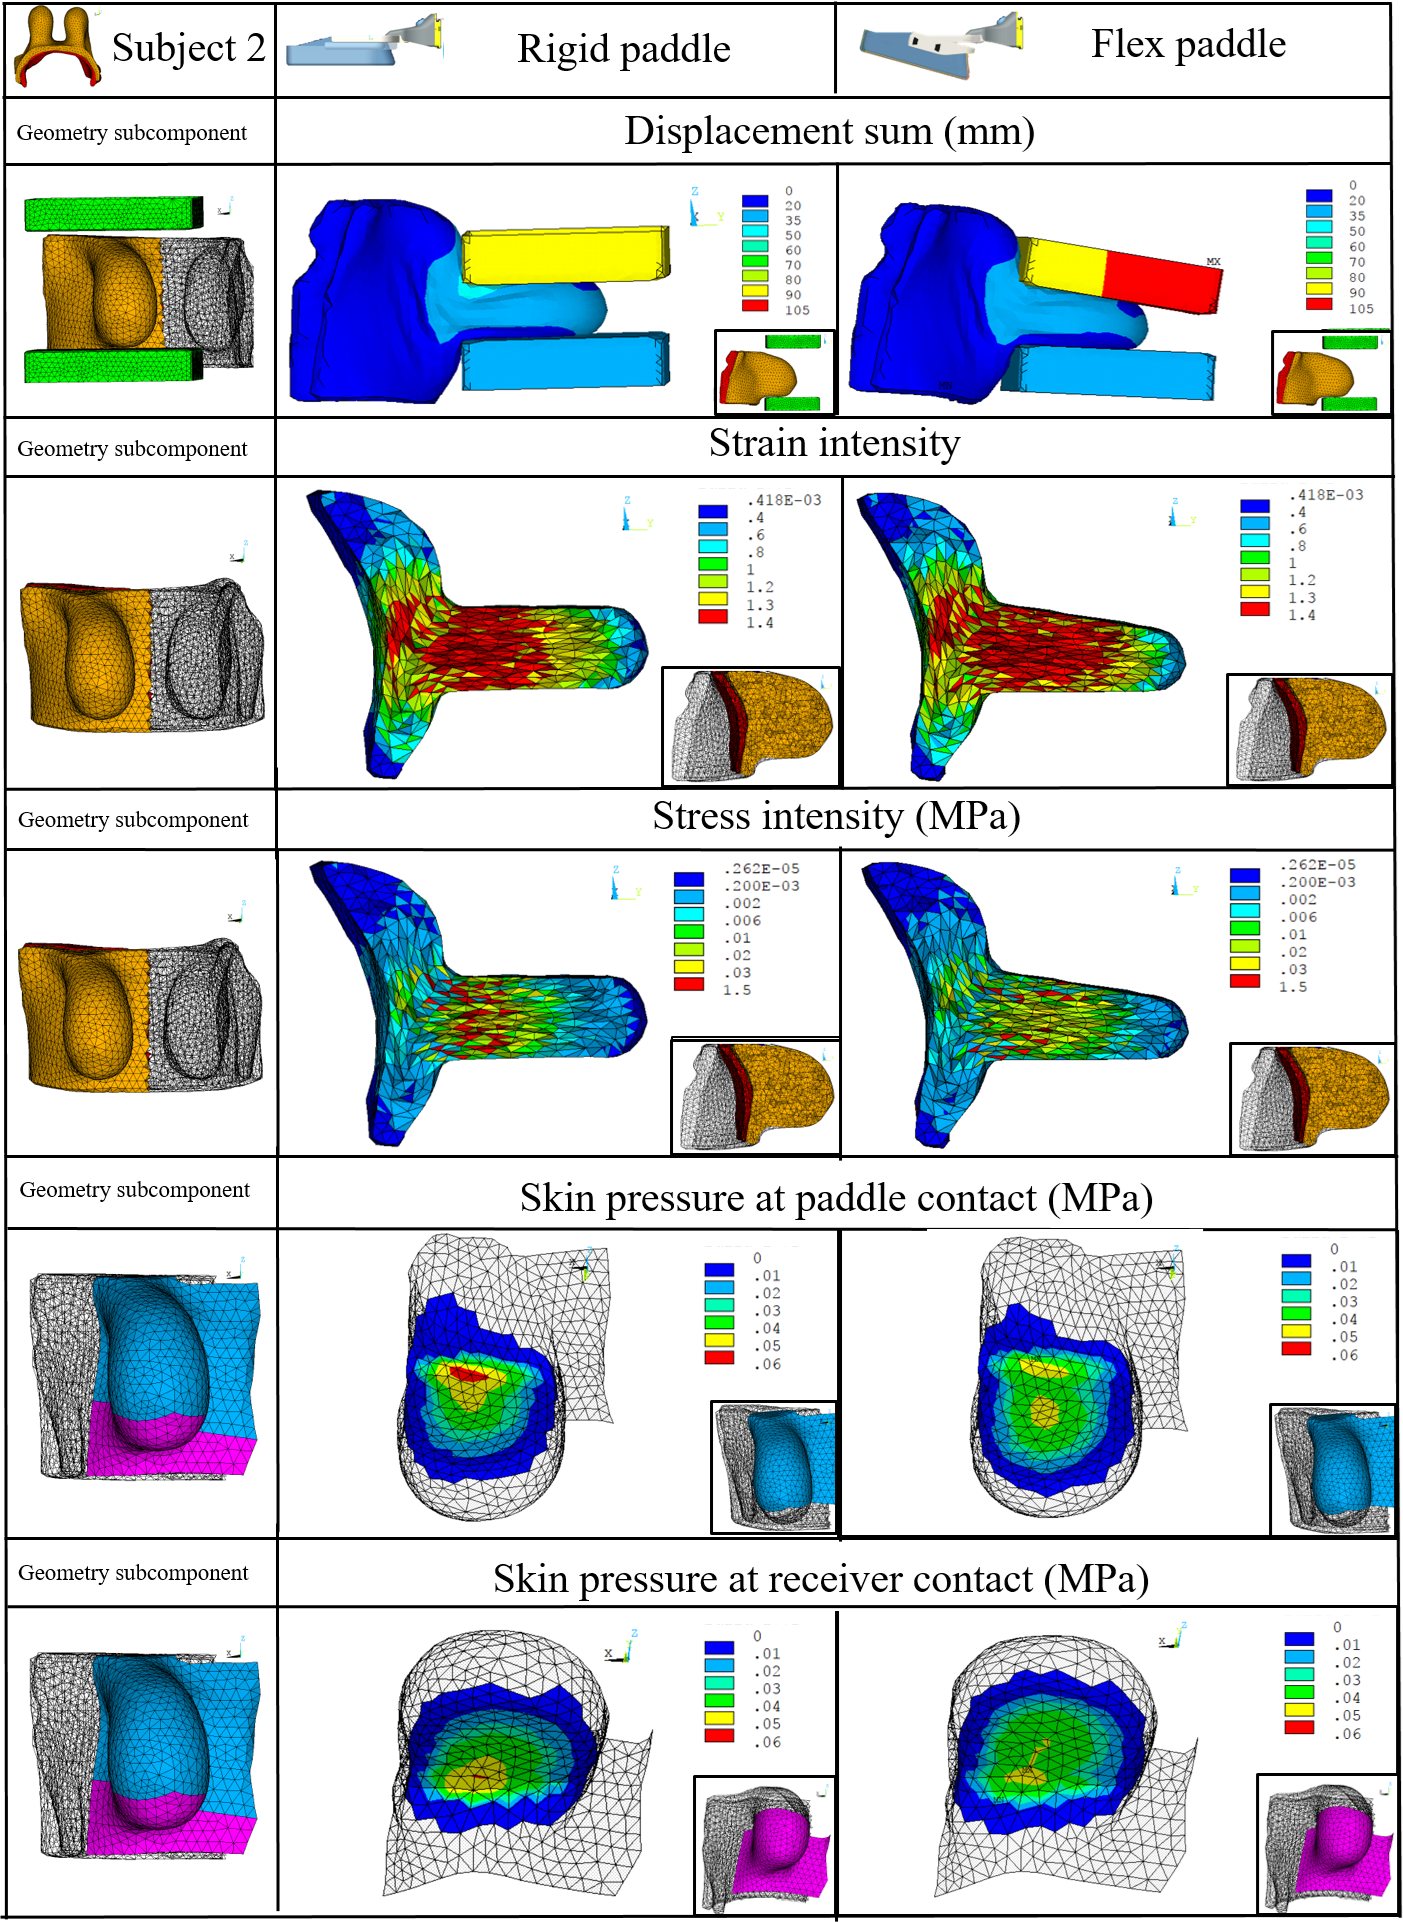
\includegraphics[width=0.9\textwidth,keepaspectratio]{figures/subject2_compressionResults.png} 
\caption{Stress, strain and contact pressure distribution for the second volunteer}\label{fig:subject2_compressionResults}
\end{figure}


Regarding the smallest breast volume (Figure \ref{fig:subject1_compressionResults}), there is no significant difference between FPM and RPM in pressure distribution over the skin surface or in internal stress/strain intensity distributions. For both compression paddles, high pressure at the skin surface is concentrated in the juxtathoracic region with a maximum pressure of 77.7 kPa. In addition, the FE simulations confirm that in small breasts the paddle tilt is too small to impact the tissues compression in the middle part of the breast. FPM applied on larger breast volumes (Figure \ref{fig:subject2_compressionResults}) results in significantly lower intensities of pressure at the skin surface in contact with the compression paddle, with a maximal pressure of 37 kPa, compared to 56 kPa when using RPM. No significant difference in the measured maximal intensities of strain and stress was observed, however strain and stress distribution patterns are different. When the breast is compressed with a rigid paddle, maximal strain and stress are concentrated in the retromammary space and decrease considerably toward the nipple. When a flex paddle is used, stress and strain are more uniformly distributed over the breast volume with the highest values in the middle third of the breast.

The area pressure distribution patterns have already been demonstrated in the work by Dustler M. et al. \citep{dustler_breast_2012}. The authors have studied the pressure distribution patterns of 103 women undergoing breast compression with a rigid paddle at different compression levels. Four groups were differentiated: a) skin pressure widespread over the breast (29\%); b) skin pressure concentrated on the central part of the breast (8\%); c) skin pressure concentrated on the juxtathoracic region (16\%); d) skin pressure concentrated along a narrow zone at the juxtathoracic region (26\%).  The pressure distribution patterns observed for our first and second volunteers correspond to the group d) and a) respectively.


\clearpage
\subsection{Paddle positioning impact on compression mechanics}\label{subsection:breastpositioning}

A second study was performed in order to assess the paddle positioning impact on the compression force. The simulations were performed only on the right breast of the second volunteer. Indeed, the geometry of the first volunteer is too small and does not meet the necessary morphological criteria required by this study. 

Using the rigid paddle model to perform compressions with different paddle position in respect to the thoracic cage (thoracic cage to paddle distance TPD, Figure \ref{fig:elasticpaddle}) has generated large convergence problems. For example, when the paddle was positioned closer to the chest wall, the finite elements were distorted because of high contact pressure at the juxtathoracic are. Therefore, for further investigations, the elastic paddle model was used. This model is closer to the mechanical properties of the standard rigid paddle from a mammography unit.  In addition, material elasticity allows a slight paddle bending which seems to reduce elements' distortions. 

\begin{figure}[!h]
\centering
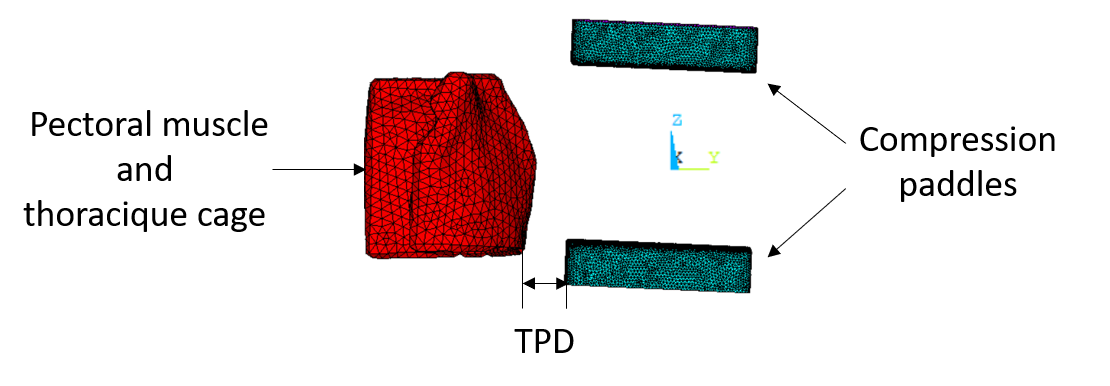
\includegraphics[width=0.8\textwidth,keepaspectratio]{figures/TPdistance.png} 
\caption{Thoracic cage to paddle distance (TPD).}\label{fig:elasticpaddle}
\end{figure}

 The breast was compressed until a minimal thickness of $50mm$ was reached. Then, the compression force as well as surface pressure at the contact with the compression paddle were compared. The compression force was computed as the product between the mean surface pressure and the contact area $\langle P_{contact}\rangle \ast  A_{contact}$.

Figure \ref{fig:elasticpaddle} shows the strain/stress as well as the pressure distributions over the contact area for three  distinct distances TPD between the paddle and the thoracic cage. The compression force varies considerably within paddle positions. A compression force of $59\ N$, $94\ N$ and $158\ N$ was obtained when the paddle was positioned at a distance from the chest wall of $48\  mm$, $40\  mm$ and $33\ mm$ respectively. Positioning the paddle with $15\ mm$ closer to the chest wall tripled the force intensity. 
 
\begin{figure}[!h]
\centering
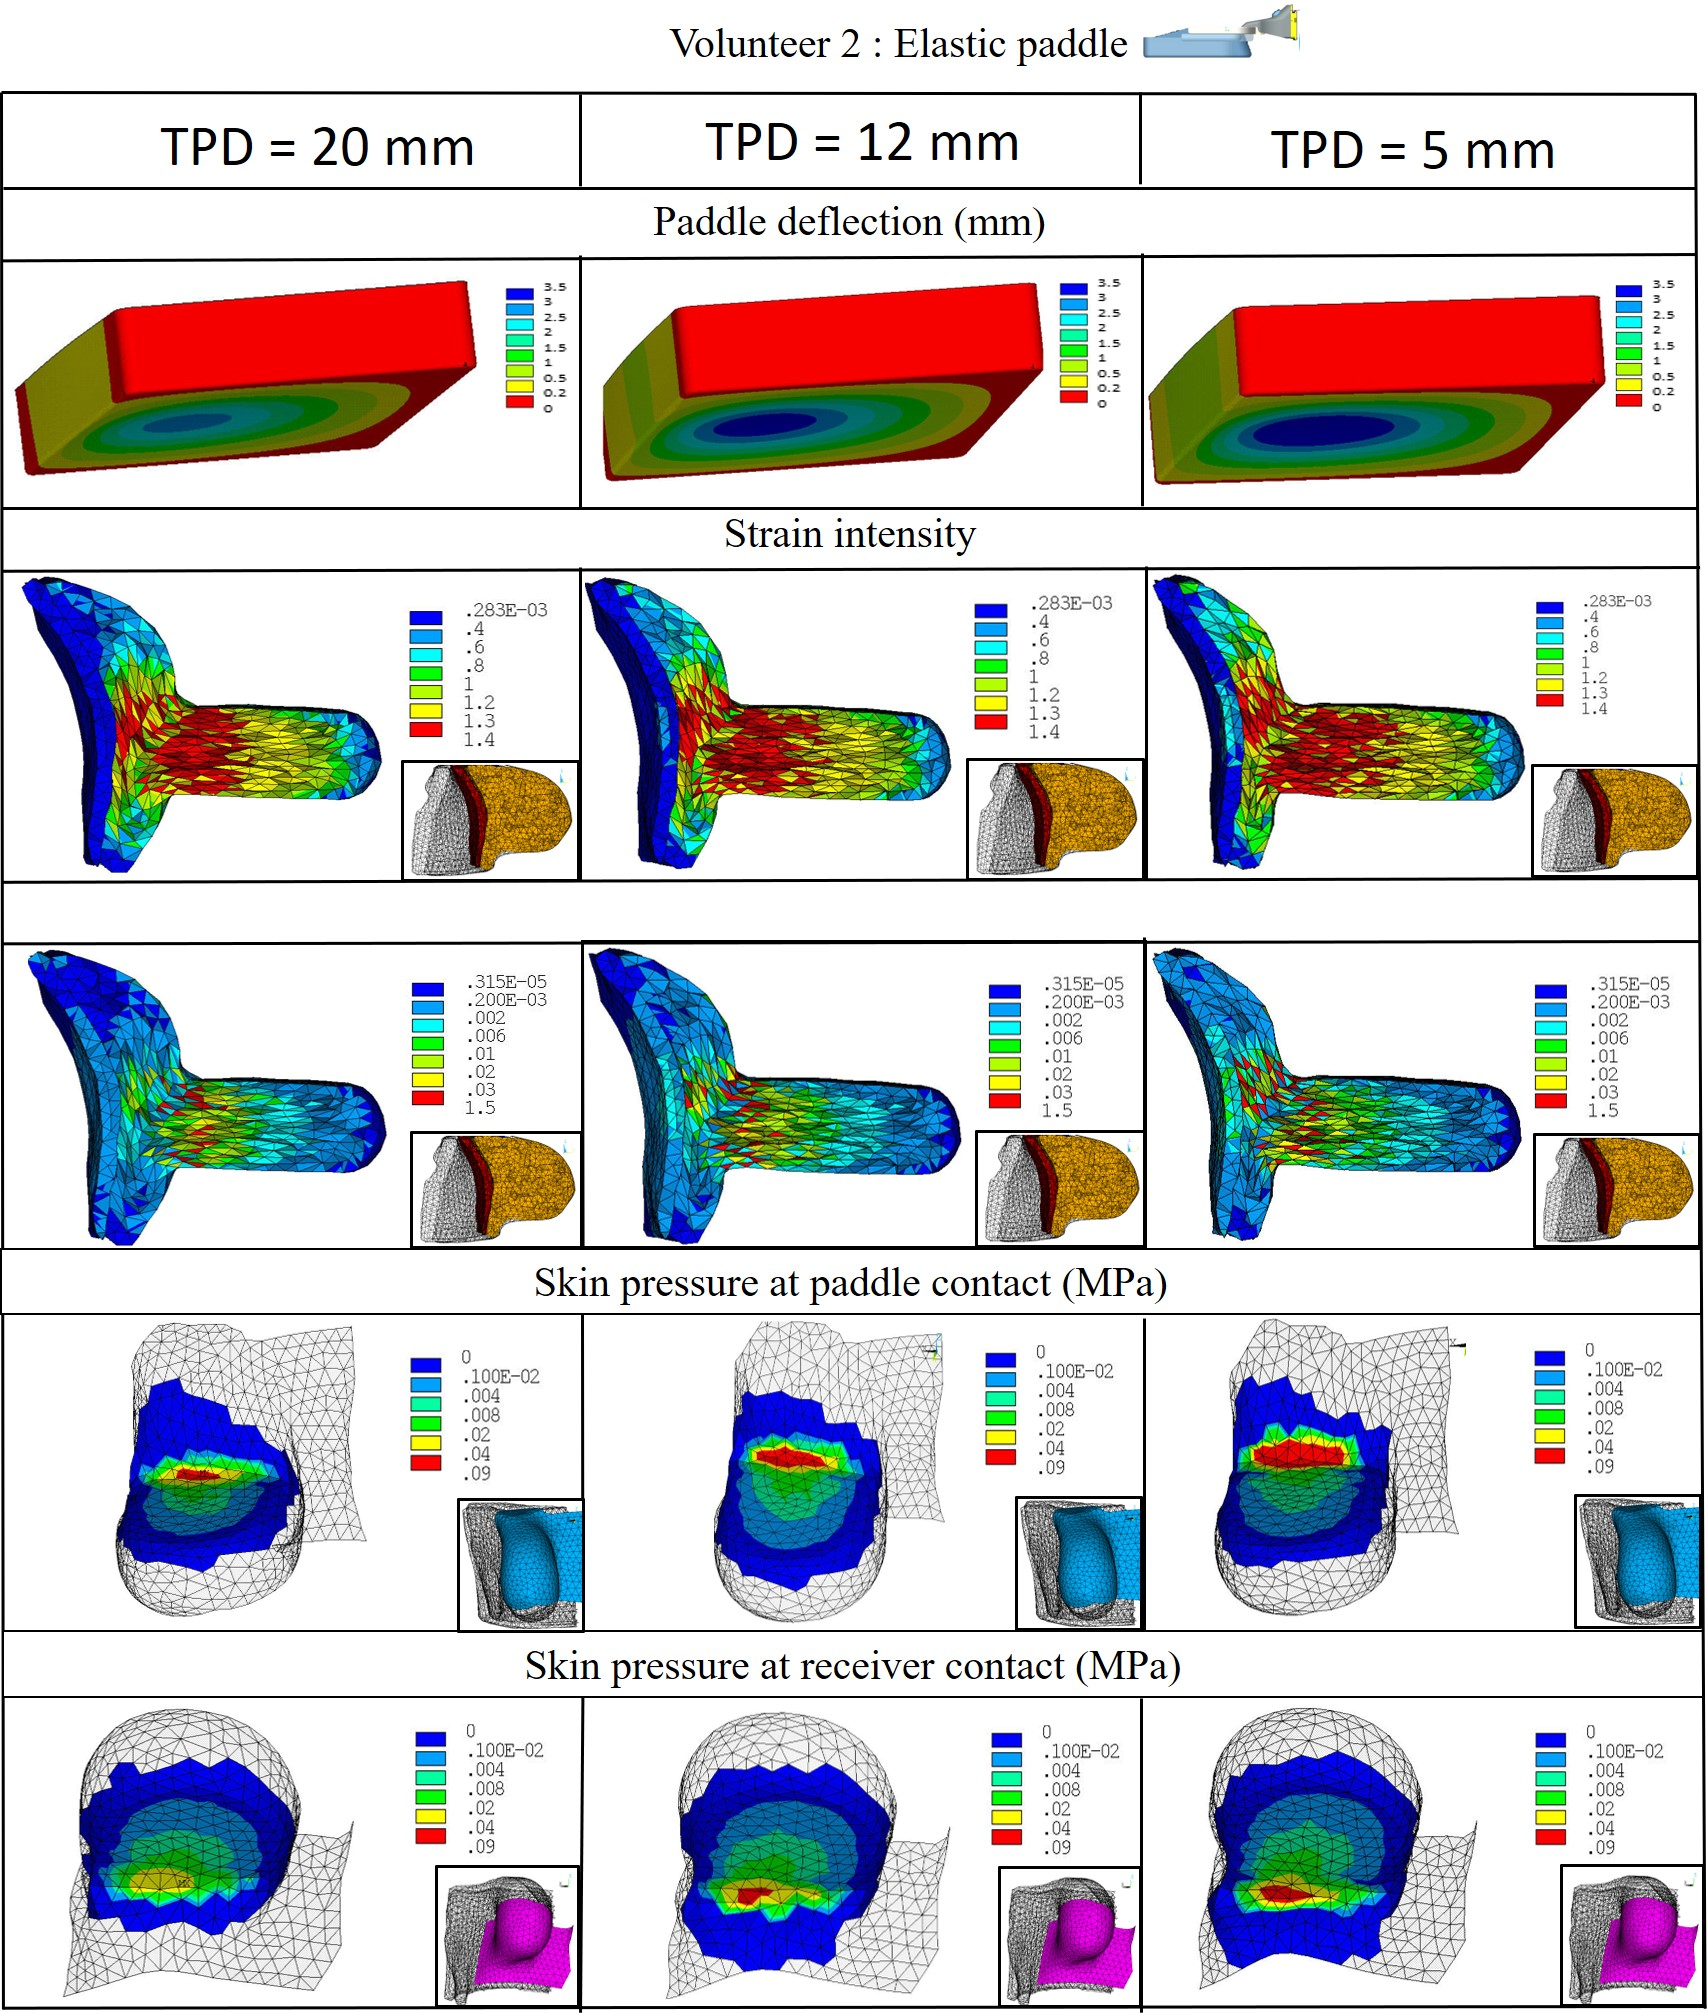
\includegraphics[width=0.9\textwidth,keepaspectratio]{figures/elasticpaddleresults.jpg} 
\caption{Stress, strain and contact pressure distribution for a variable thoracic cage to paddle distance (TPD).}\label{fig:elasticpaddle}
\end{figure}


Due to the paddle elasticity, the breast thickness slightly varies, with a maximal deflection equal to $3.5\ mm$ (Figure \ref{fig:elasticpaddle} first line). A very small difference between the maximal paddle deflection  $(\sim 1\ mm)$ was observed within the previous three compressions. Thus, image quality or AGD were not significantly impacted by the breast thickness variation. However, the wider the space between the chest wall and the compression paddle, the fewer breast tissues in the projected mammography image. In a standard framework, the technologist will include as much breast tissues as possible in order to reduce the risk of missing a suspicious lesion.

When looking at the strain distribution, one can see that, when the compression paddle is positioned closer to the chest wall, the juxtathoracic soft tissue undergoes higher deformation resulting also in a higher stress intensity. Concerning the skin surface pressure distribution, the highest intensities $ (\sim 90\ kPa)$ are always concentrated in the juxtathoracic area. However, for a thorax to paddle distance equal to $33\ mm$, the area corresponding to the high pressure is considerably larger. This means that a significant part of the total force was  used to compress the tissues in the juxtathoracic area only, which may increase the patient discomfort.

\section{Discussion and conclusion}\label{section:compressionfem:conclusion}

In this chapter, the breast compression was simulated using three paddles models, the rigid, flex and elastic models. In order to comply with the compression mechanics as described in literature, an update of the tissues constitutive models was needed. Appling the Gent form of strain-energy potential, instead of the Neo-Hookean form, allowed to obtain compression force magnitudes comparable with the real subject data. However, when the same law is used to perform the multi-loading gravity simulations, the breast deformations in supine and prone configurations are over-constrained. We found that, with a larger value of $J_m$ parameter, the Gent model may improve the breast geometry estimates obtained with a Neo-Hookean model.
In conclusion, the estimated value of $J_m$ does not characterize the subject-specific mechanical properties and gives only an estimation of a standard behaviour.  Our second study shows that, to obtain a proper estimation of parameter $J_m$, more information like the paddle position with respect to the breast volume is needed. 

The patient comfort (measured as strain and stress) as well as the image quality (measured as SNR, SDNR ) and AGD were compared for breast compression with rigid and flex paddles. The results from the two volunteers were analysed. The compression simulations indicate that, for the smallest breast, there is no significant difference for the patient perceived pain when using the rigid or the flex paddles. We did not observe any statistically significant difference in SNR or SDNR for microcalcification of any size. Therefore, our results suggest that using a flex paddle should not significantly impact image quality and delivered dose in small breasts and should not reduce significantly the perceived pain.   
For the largest breast, our simulations indicate that using a flex paddle may reduce the maximal pressure intensity on the skin surface by about 30\% compared to the rigid paddle. The tissues deformation is more uniformly distributed inside the breast volume, and the highest deformation occurs in the middle breast region corresponding to the supposed location of dense tissues. Moreover, our simulations have shown that the flex paddle has no significant impact on the average glandular dose and improves image quality compared to the rigid paddle. However, breast compression with a flex paddle is suspected to facilitate the displacement of the fibroglandular tissues into the retromammary area. As the breast thickness increases linearly from the nipple to the chest wall, the retromammary area is characterized by a low image quality. 


The impact of paddle positioning on patient comfort and image quality was also addressed. Three paddle positions with respect to the chest wall were studied using the elastic compression paddle. Even if a variable breast thickness is obtained due to the paddles deflection, the variations are too small ($\sim 1mm$) to impact the AGD or the resulting image quality in terms of the SNR or SDNR. However, by excluding the retromammary tissues from the imaged area, information on small posterior cancerous legions may be lost. In terms of patient comfort, the simulations have shown that the high pressure are always localized in the juxtathoracic areas. When the paddle is too close to the chest wall, the compression force is mostly dissipated on this narrow area resulting in very high pressures compared to the skin pressure over the breast ($90kPa\ vs\ 10kPa$).


\clearemptydoublepage
\part{Thesis review}\label{part:thesisreview}

\chapter*{Conclusion}\label{section:generalconclusion}
\addcontentsline{toc}{chapter}{Conclusion}
\cleardoublepage
\chapter*{Perspective}\label{section:perspectives}
\addcontentsline{toc}{chapter}{Perspective}

 This simulation environment will allow us not only to evaluate the existing compression techniques, but also to perform a first evaluation of new, not yet conceived, paddles designs at a numerical level. 
 \cleardoublepage
\chapter*{Key contributions}\label{section:keycontributions}
\addcontentsline{toc}{chapter}{Key contributions}
\cleardoublepage



%\chapter{State of the Art}\label{chapter:stateoftheart}
%\input{chapters/stateoftheart}
%\clearemptydoublepage

%\chapter{Report}\label{chapter:validation}
%
\section{Abstract}
The purpose of this work is to study the feasibility of digital breast tomosynthesis (DBT) with reduced breast compression. The actual compression method will be investigated using a biomechanical breast model. The compression methodology is reproduced by means of finite element theory in order to estimate the impact of the non-uniform breast thickness on the image quality and the average glandular dose. First, the breast 3D biomechanical model is the subject of a hyper-elastic transient simulation within the ANSYS software. Second the compressed model is imported in CatSim simulation framework for X-ray computed tomography, and synthetic images are generated. Finally, the correlation between the phantom thickness and image parameters is analyzed. The biomechanical breast model will be also used to estimate the perceived pain in terms of tissues internal strain due to compression.
 Based on the analysis results, alternative compression methods will be investigated in order to improve the patient comfort and cheep a good lesion detectability and a low average glandular dose.

In this scope a biomechanical breast model has first been developed and is currently validated based on MR images of 3 volunteers. The proposed model takes into account breast heterogeneity, hyper-elasticity and patient specific geometry and tissues elasticity. Four types of tissues are highlighted: muscle, adipose tissue, glandular tissue and skin. All breast tissues are modelled as neo-Hookean materials. A particular attention is granted to modelling the breast support matrix computed of the fascia membrane. A physical correct modelling of the breast requires the knowledge of the stress-free breast configuration. Here, this reference shape (i.e. without any internal stress) is computed using an adapted prediction-correction iterative algorithm. 


\section{Introduction}
Mammography is a specific type of breast imaging that uses low-dose X-rays to detect cancer in early stage. During the exam, the breast is compressed between two plates until a nearly uniform breast thickness is obtained. This technique optimizes image quality, hence the tissue visualization and reduces the absorbed dose of ionizing photons.  But breast compression is also often a source of discomfort and sometime pain for the patient during and after the exam. Though the mammography is the most effective breast cancer screening method, the discomfort perceived during the exam could deter women from getting the test. Therefore, alternative techniques allowing reduced breast compression is of potential interest.

The aim of this work is to develop a 3D biomechanical Finite Element (FE) breast model in order to analyze various breast compression strategies and their impact on image quality and radiation dose. CatSim environment is used to create artificial breast images from numerical phantoms and to compute the corresponding averaged glandular dose. The biomechanical model estimates the compressed phantom geometry relative to the applied forces before being introduced in the image simulation workflow. From the finite element solution, the 3D strain cartography is computed as a first guess of pain and discomfort.
\subsection{Finite element breast models}
Biomechanical modelling of breast tissues is widely used in various medical applications such as surgical procedure training, pre-operative planning, diagnosis and clinical biopsy, image guided surgery and image registration, material parameter estimation. For the last 20 years several research groups have presented their breast models based on finite elements theory. One of the first breast biomechanical models based on the finite element theory is the one proposed by \cite{azar_methods_2002}. The model is used as a novel method for guiding clinical breast biopsy. The breast tissue is considered homogeneous, isotropic, incompressible and modeled as a non-linear material. The compression is modelled using virtual compression plates by applying displacements to the surface nodes. Large deformation is approximated by a sum of small increments using small-strain considerations.

Later more complex models where developed implying different types of tissues, anisotropies, large deformation theory and more complex boundary conditions. \cite{rajagopal_development_2004} developed a model based on large deformation mechanics in order to validate the assumption of isotropy, homogeneity and incompressibility of soft tissues. The material models where computed using the bibliography data only. The method was validated experimentally using silicone gel phantoms subject to gravitational loading. \cite{rajagopal_modelling_2007} also studied the effect of modelling the breast skin layer. And as \cite{pathmanathan_predicting_2008} research team they found that modelling the skin results in an underestimation of breast displacements. 

\cite{han_development_2012} developed a bio-mechanical breast model for surgical simulations. In their model 3 types of tissues are considered: muscle, glandular and adipose tissues. \cite{gamage_modelling_2012} introduced the pectoral muscle in the breast mechanical model and showed that the muscle should be accounted in the modelling.

 The anisotropic effect of Cooper's ligaments was introduced for the first time by \cite{pathmanathan_predicting_2008} and took up again by \cite{han_development_2012}. Both teams have introduced an additional factor in the stress-strain energy function describing the transverse isotropic properties. They also	 considered the breast heterogeneity by modelling adipose tissue and fibro-glandular tissues with different materials. However, the model was not validated using clinical data. A new modelling method for Cooper's ligaments vas proposed by \cite{georgii_simulation_2016}. They added a generic ligaments model based on a mass-spring system to the finite element model. 
 
 The deformation of an elastic body is typically performed by specifying appropriate boundary conditions. Almost all biomechanical breast models are based on fixed boundary conditions, i.e. the nodes lying on the posterior face of the breast are defined with zero-displacement proprieties.
\cite{payan_application_2012} replaced the "fixed" boundary conditions by a "sliding" region between the posterior part of the breast and anterior part of the pectoral muscle. Recently the \cite{patz_sliding_2015} team have presented a new time-preserving method to model the sliding motion. The sliding method is based on fixed boundary conditions in conjunction with an explicit update computed using the resulting internal forces of the elastic material.

The bibliography presents 3 main limitations for breast mechanical simulation:
\begin{enumerate}
\item Unknown stress-free breast configuration. Since, for all in-vivo studies, breast geometry is extracted from the MRI data, the measured configuration represents the breast subject to gravity loading. Thus, for a Finite Element modeling it is very important to accurately estimate the unloaded (i.e. stress-free) configuration.
\item Unknown elastic parameters of breast soft tissues. The bibliography shows a very large interval of elastic parameters depending of the experimental methods and made assumptions.
 \item Breast tissues are known to be extremely soft. Very large deformation of materials implies excessive elements distortion. A poor mesh quality can lead to inaccurate results and numerical instability.
\end{enumerate} 

\subsection{Breast tissue biomecanical modeling}
Global breast mechanics are governed by breast tissue compositions and their individual mechanical properties. Therefore, an accurate breast model stands on a good knowledge of breast anatomy and on full characterization of the mechanical behavior of the involved tissues.

 Multiple studies have show that female breast composition and so its mechanical behavior undergo substantial changes during the lifetime.
The first studies on estimation of mechanical proprieties of breast tissues were done in diagnostic purposes. Presence of tissues with mechanical proprieties different from the breast-like tissues implies breast anomalies. The study published by \cite{krouskop_elastic_1998} show the difference in stiffness between breast tissues and carcinomas. In this study authors supposed that the difference in breast global stiffness is only due to the changes in breast tissues compositions and not in changes of the individual material property. Therefore, they have studied ex-vivo 142 tissues samples from different subjects and they assumed their homogeneity. The samples were representing 4 type of tissues: adipose tissue, glandular tissue, fibrous tissue and carcinoma. They showed that due to the difference in material stiffness measured using elastography they are able to detect pathological changes in breast tissues and moreover they can estimate elastic parameters of normal tissues images from elastography.  

%Later  

 Later, several research groups have presented values of elastic modulus of adipose and glandular tissues. The range of elastic parameters is going from 0.1 kPa to 271.8 kPa (see table \ref{elastic_modulus_table}). Such big variation can be explained by the differences in the used methods but also by the different physical condition, age or period of the menstrual cycle of the participants. \cite{lorenzen_menstrual-cycle_2003} found that during the menstrual cycle, due to the hormonal changes, the elastic properties of the glandular tissues can change by about 30 \%. 
%\begin{table}[h]
\begin{sidewaystable}
    \centering
   \begin{tabular}{c|c|c|c|c}
   \hline
  \multicolumn{5}{c}{\textbf{Ex-vivo estimation}}\\
   \hline
    Author & Method & Material model&\multicolumn{2}{c}{Material constants} \\
    \cline{4-5}
    &&& Adipose & Glandular\\
    \hline
    \cite{krouskop_elastic_1998} - 5\% precomp. & identation & Linear elastic & E=20 kPa & E=33 kPa \\
    \cite{krouskop_elastic_1998} - 20\% precomp. & identation & Linear elastic & E=20 kPa & E=57 kPa \\
    \cite{wellman_breast_1999}- 5\% precomp. & identation & Linear elastic & E=6.6 kPa & E=33 kPa \\
    \cite{wellman_breast_1999}- 15\% precomp. & identation & Linear elastic & E=17.4 kPa & E=271.8 kPa \\
     \cite{samani_elastic_2007} & identation & Linear elastic & E=3.25 kPa & E=3.24 kPa \\
   \hline
  \multicolumn{5}{c}{\textbf{In-vivo estimation}}\\
   \hline
     \cite{van_houten_initial_2003} & MRE & Linear elastic & E=17-26 kPa & E=26-30 kPa \\
     \cite{carter_determining_2009} & MRI & Neo-Hookean & $C_{10}$=0.2-1 kPa & $C_{10}$=0.4-0.8 kPa \\
     \cite{han_development_2012} & MRI & Neo-Hookean & E=1 kPa & E=0.22-43.64 kPa \\
     \cite{gamage_modelling_2012} & MRI & Neo-Hookean & $C_{10}$=0.1 kPa & $C_{10}$=0.1 kPa \\
     \cite{Rajagopal_creating_2008} & MRI & Neo-Hookean & $C_{10}$=0.08 kPa & $C_{10}$=0.13 kPa \\
    
    
    \end{tabular}
     \caption{Elastic modulus of adipose and glandular tissues}
     \label{elastic_modulus_table}
\end{sidewaystable}
%\end{table}

An important difference in the estimated elastic modulus of soft tissues is observed between the linear elastic and hyperelastic models. In the l studies where authors are using a hyperelastic Neo-Hookean models with in-vivo measurements, the range of the adipose and glandular elastic modulus is lower than 1kPa, compared to an average of 20-30 kPa given be the linear models with ex-vivo measurements. 

\cite{carter_determining_2009} used a Finite Element breast model considering 3 types of tissues: adipose tissue, glandular tissue and skin. All 3 tissues were modelled as Heo-Hookean incompressible materials. Since the soft tissues are of the same density as the water, the submerged in water breast was considered to have zero internal stress.  The elastic parameters are estimated by minimizing the difference between computed and measured prone breast configurations. For this model the authors obtained elastic modulus equal to 0.2 kPa for adipose tissue, 0.4 kPa for glandular tissue and 10 kPa for skin.

 \cite{gamage_modelling_2012} have considered the breast as a homogeneous material but have also included the pectoral muscle in the biomechanical model. Both tissues were modelled as hyperelastic materials. They obtained 0.1 kPa for elastic modulus of the homogeneous breast and 0.52 kPa for muscle. 
  
 \cite{van_houten_initial_2003} have considered also the Poisson Ratio as a variable. The estimation is done in in-vivo conditions (based in magnetic resonance elastography). The authors assume linear material behavior therefore the elastic modulus and Poisson Ratio are computed from the 2 Lam\'e modulus. They found that the Poisson Ratio for adipose tissue lies between 0.34-0.4 and for glandular tissue around 0.4.

Previously listed researches clearly showed the variability of elastic modulus of the same tissue between and within individuals. \cite{eder_comparison_2014} made a large analysis of all existing material models. According to their findings many of proposed in the literature parameters are too stiff, and namely those that are obtained by indentation ex-vivo test. The more reliable values are given by \cite{Rajagopal_creating_2008}, the other values permitting not enough deformation due to the gravity loading.
\subsection{Skin biomechanical modeling}
The skin mechanical parameters are also important in breast mechanics. Only \cite{carter_determining_2009} have included the skin in the identification process of the breast soft tissues elastic modulus. The authors modeled the skin as a Neo-Hookean incompressible material, and they obtained an elastic modulus equal to $10kPa$. 

\cite{sutradhar_vivo_2013} published a complete study of breast skin estimating the thickness and elasticity for 16 different breast regions. The study was done on 23 female volunteers aging from 29 to 75 ears. With in-vivo suction experiments they found an average thickness of $1.55mm$ and an elastic modulus of 334kPa. They also showed the regional variation of skin thickness: according to the authors the lateral region thickness is the thinnest among all the breast regions followed by superior/inferior part (without any significant differences) and the medial region. Concerning the radial distribution, the interior region closer to the nipple was more thin than the exterior radial part of the breast. A similar regional variation study was done on the skin elasticity. It was found no significant variation of elastic modulus in radial direction. The modulus was found grater in the superior and lateral part than in the inferior and medial parts respectively. An additional measurement was done in order to compare the skin elastic modulus in supine and upright position with no significant differences found.

 Other research on skin elasticity are available, but they are not specific to the breast skin. \cite{hendriks_relative_2006} estimated in-vivo skin proprieties by suction testing. The skin was considered as a homogeneous, isotropic, incompressible, hyperelastic material. The study was performed on 14 subjects and the obtained average of elastic modulus for skin was $58,4 kPa$.  

\subsection{Stress-free breast configuration}
As mentioned before, in the breast configuration given by MR images the soft tissues are pre-stressed due to in-vivo conditions (i.e gravitational forces). In order to apply the continuum mechanics theory, an initial stress-free breast shape is needed. 

One of the existing methods for estimating such a stress-free shape is the backward finite element formulation used by \cite{pathmanathan_predicting_2006} in his biomechanical model. The method is based in the reformulation of the virtual work equation, where the residual forces are expressed in terms of unknown reference state coordinates. 

\cite{carter_biomechanical_2009} addressed the same problem solving an iterative sequence of forward deformations where the only unknown is the reference configuration. First, the reference configuration is assumed to be equal to the prone breast configuration. Second the gravity loading is applied in order to compute a first estimation of the prone configuration. From the first estimation of deformed state a difference in node location is computed. Then, the reference state is perturbed accordingly to the computed difference until convergence is achieved.

 Later \cite{eiben_breast_2014} refined the method by translating the difference location vector from the deformed space to the reference space by multiplying the vector with the inverse deformation gradient.   \cite{eiben_breast_2014} compared the two previous methods; according to the authors the backward formulation methods exhibits excellent results only when elastic parameters are well known. Since in the prone-supine breast deformation context the elastic parameters are unknown, there is no significant numerical difference between the two methods.   
 
  This problem was raised for the first time by \cite{kuhlmann_mechanical_2013}. To solve the large deformation problem, they proposed a coupled Eulerian-Lagrangian FE method. According to the authors this method is more relevant for breast soft tissues but is highly time-consuming.   
 

\section{Materials and methods}
\subsection{Breast Anatomy}

A good knowledge of anatomical breast structure and its composition is necessary when one is developing a biomechanical model.  The tissues distributions and their biomechanical properties define the global breast mechanics. 

 \subsubsection*{Breast embryogenesis}
The breast gland have the same ectodermal origin  as skin glands.

\begin{center}
\begin{figure}[!htb]
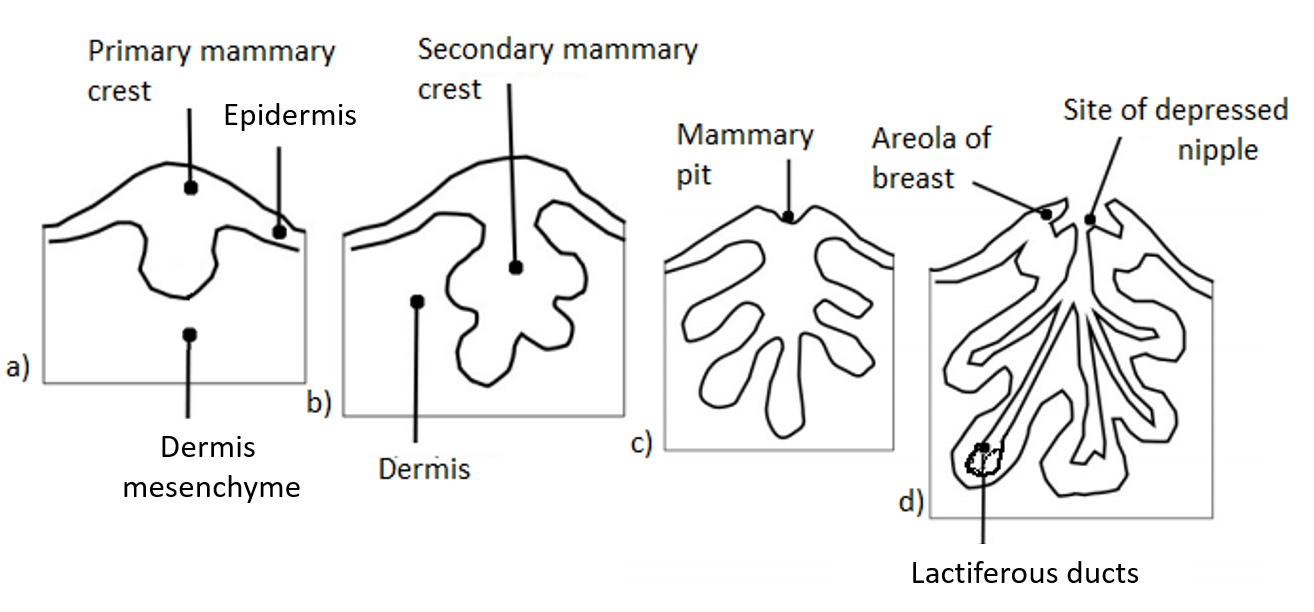
\includegraphics[width=\textwidth,height=\textheight,keepaspectratio]{figures/breast_evolution_my.png} 
\caption[Breast embryogenesism: stages of formation of the duct system. the ectoderm is responsible for duct system and alveoli, the mesenchyme is responsible for the connective tissue and vessels] {Breast embryogenesism: stages of formation pf the duct system. the ectoderm is responsible for duct system and alveoli, the mesenchyme is responsible for the connective tissue and vessels  ~~ ~\cite{shiffman_melvin_a_breast_2008}. }
\label{breastembryogenesis}
\end{figure}
\end{center}

 During the first trimester of intrauterine growth,  the mammary crest develops in the embryo ectoderm (fig \ref{breastembryogenesis}.a), 16-24 solid cords of epithelial cells are growing down into the dermis (fig. \ref{breastembryogenesis}.b). Later, these cords will evolve in the lactiferous ducts and alveoli (fig. \ref{breastembryogenesis}.d). At the full-term fetus there is already a simple network of branching ducts. The glandular elements, generally do not appear until adolescence. In the adolescence, under hormonal simulation, the breast buds enlarge on the chest wall and eventually on the axilla region , becoming palpable discs beneath the nipple. The ducts grow into the soft tissues and the lobular differentiation begins \cite{kopans_daniel_b_breast_2007}. 

\begin{center}
\begin{figure}[!h]
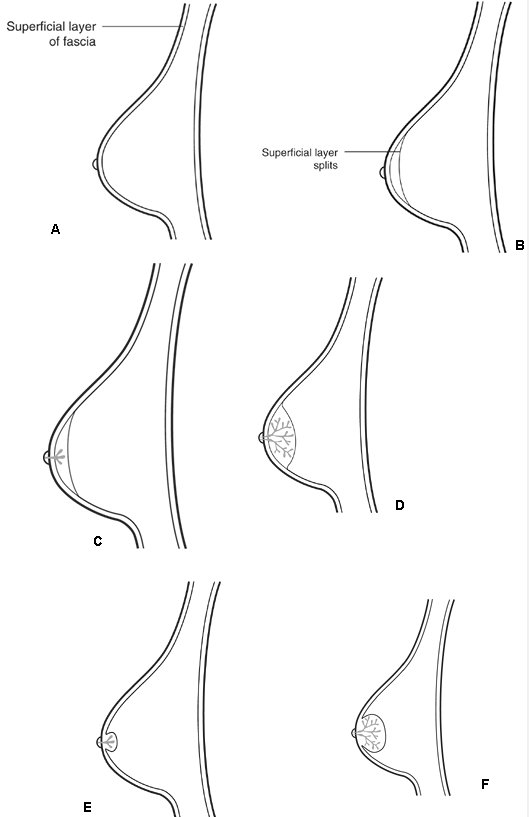
\includegraphics[height=0.7\textheight,keepaspectratio]{figures/breastEvol_fascia.png} 
\caption[Breast development sequence in the subcutaneous tissues. A-D Mammary bud development by spleeting the superficial fascia in 2 layers. E-F Mammary bud development]{Breast development sequence in the subcutaneous tissues. A-D Mammary bud development by sleeting the superficial fascia in 2 layers. E-F Mammary bud development, reproduced from  ~~\cite{kopans_daniel_b_breast_2007}  }
\label{breastevol_fascia}
\end{figure}
\end{center}

\cite{kopans_daniel_b_breast_2007} analyzed breast development sequence in the subcutaneous tissues. According to the author the evolution of breast within the fascial system is unclear, two possible evolution are presented: 
\begin{enumerate}
\item The superficial fascia split in two layers forming the deep and the superficial fascia layers. With the breast forming in between (fig.\ref{breastevol_fascia}.A-D).
\item The elongating ducts invaginate the fascia which end up 
enveloping the gland (fig.\ref{breastevol_fascia}E-F)
\end{enumerate}


\subsubsection*{External structure}
The breast is an apocrine, tear-shaped gland \cite{valerie_mammographic_2011}. Anatomically, the adult breast sits atop the ribcage, between the clavicle and the sixth to eighth ribs. The breast tissue extends horizontally (side-to-side) from the lateral sternal line out to the midaxillary line (see fig.\ref{fig:breast_quadrants}).

The adult breast size variates within intra and inter individuals. The asymmetric breast within individuals is relatively usual. Therefore some research groups have defined geometry metrics in order to characterize the variation of breast size  and its asymmetry. By definition the base of the breast is the portion adjacent to the chest wall, the apex is the nipple-areola complex (fig. \ref{fig:breast_apex}), the breast projection is the distance from the apex to the breast base. 


\begin{figure}[h]
\minipage{0.1\textwidth}
\endminipage\hfill
\minipage{0.5\textwidth}
  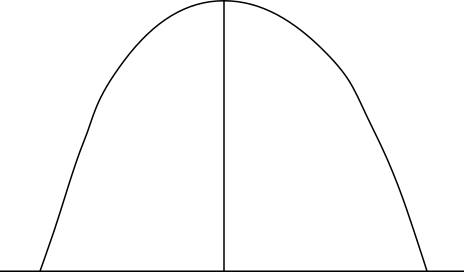
\includegraphics[width=\linewidth]{figures/breastBase.PNG}
  \caption{Base and apex of the breast}\label{fig:breast_apex}
\endminipage\hfill
\minipage{0.2\textwidth}
  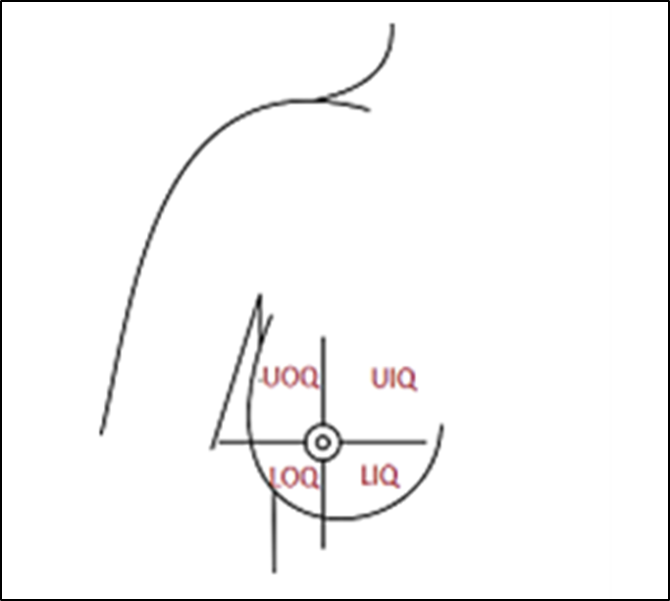
\includegraphics[width=\linewidth]{figures/Breast_quadrants.png}
  \caption{Four breast quadrats}\label{fig:breast_quadrants}
\endminipage\hfill
\minipage{0.1\textwidth}
\endminipage\hfill
\end{figure}
In medical imaging, to describe location in the breast, four quadrants are defined: upper outer quadrant (UOQ), upper inner quadrant (UIQ), lower outer quadrant (LOQ), lower inner quadrant (LIQ)(see fig.\ref{fig:breast_quadrants}).   The natural landmarks of thorax surface are the nipple, the inframammary fold, the jugular notch, clavicle, sternal angle and the axilla. Some of these structures are used to describe locations of normal anatomy and pathology.

\begin{center}
\begin{figure}[!h]
\centerline{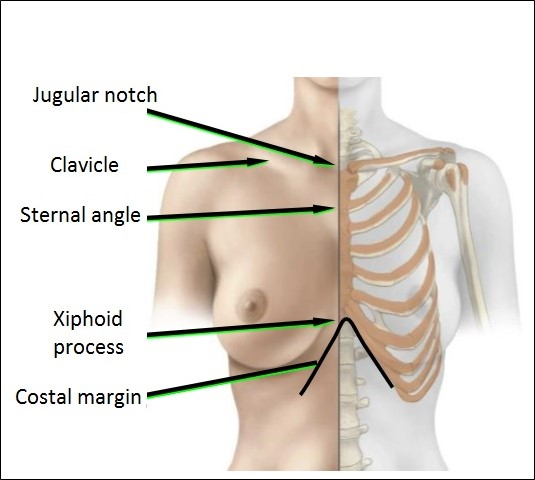
\includegraphics[width=0.5\textwidth,height=0.5\textheight,keepaspectratio]{figures/surfacelandmarks.jpg} }
\caption{Thorax surface landmarks.}
\label{thorax}
\end{figure}
\end{center}

Studies on the breast dimensions have been done essential for cosmetic and reconstructive surgery. \cite{catanuto_experimental_2008} presented several parameters which can characterize unambiguously the breast shape, among them the curvature of the thoracic surface has been identified as the most relevant. The superior half of the healthy breast was shown to be
almost flat especially in the inner quadrants (fig. \ref{fig:breast_quadrants}) while moving towards the upper outer quadrants curvature becomes negative. According to the authors, the breast deformation can not be described by volume measurements only.

The skin is the covering breast layer which provides protection and receives sensory stimuli from the external environment. It is a heterogeneous organ composed of 3 layers, see fig. \ref{skinanatomy} (\cite{gefen_mechanics_2007}): 
\begin{enumerate}
\item epidermis (dead cells) mainly composed of keratin, it's thickness ranges between 50 and 100 $\mu$m ;
\item dermis: composed of collagen and elastin fibers in a viscous matrix made of water and glycoproteins, with a thickness between 1-3 $mm$;
\item hypodermis, mainly composed of adipocytes cells, it's thickness variate depending on the individual and location area between 1 and 7 $mm$.
\end{enumerate}


\begin{center}
\begin{figure}[!h]
\centerline{\includegraphics[width=0.5\textwidth,height=0.5\textheight,keepaspectratio]{figures/skin.jpg} }
\caption{Skin anatomy}
\label{skinanatomy}
\end{figure}
\end{center}


The breast skin is thickest at the base of the breast ($\sim$ 2 $mm$), and becomes thinner approaching to the nipple ($\sim$ 0.5 $mm$) (fig. \ref{breastanatomy}). At the nipple areola region, the skin thickness measure 4-5 $mm$ (\cite{valerie_mammographic_2011}). \cite{ulger_harun_effect_2003}
described the range of normal breast thickness using a film-screen mammographic technique. According to the authors the breast skin ranges between 0.50 mm and 3.10 mm, with significant differences between the 4 regions in the same breast. They also found that, even if the breast size increases with age, the skin thickness decreases in all regions.

\subsubsection*{Internal structure}

Breast heterogeneous structure includes a mixture of parenchyma and adipose tissue (see fig. \ref{breastanatomy}). The breast parenchyma consists of: glandular components, lymphatic network and blood vessels (\cite{clemente_anatomy:_2011}). Cooper's ligaments and fascias are the supporting system of the breast, their interconnection and intersections with the pectoral muscle fix and support the breast soft tissues.

 A layer of adipose tissue and connective fascia separates the breast from the pectoral muscle forming a retro-mammary fat space. Adipose tissue is also the predominant tissue of the breast that fills up depressions between the two layers of fascia. In the intra-fascial space, fatty tissue surrounds and is dispersed among the glandular structures \cite{valerie_mammographic_2011}. Fat properties and its spatial distribution gives the breast a soft consistency. The amount of fat determines the size of the breast. The aim of this tissue is to protect the lobes and the lactiferous ducts.

Glandular tissue is represented by breast lobes. A healthy female breast is made up of 12-20 lobes. They are distributed centrally and laterally within the breast. The total amount of glandular tissue depends on the hormonal fluctuation, age and physical state.  Mammary ducts arise from the lobes as branches and connect them to the female nipple. There are about 10 duct system with a tree-like structure in each breast that carry the milk from the lobes to the nipple. The dark area of skin surrounding the nipple is called the areola. \cite{huang_shih-ying_characterization_2011} have studied the breast shape and fibro-glandular distribution using dedicated breast CT images. This study shows that the glandular tissues is situated in the central portion of the breast. In prone position about 60 $\%$ of glandular tissues is located near to the nipple. A mean percentage of glandular tissue was computed by \cite{yaffe_myth_2009}, the values varied from 13.7$\%$ to 25.6 $\%$ within different groups. They also mentioned a drop in glandular fraction with the advancing age. 


\begin{center}
\begin{figure}[h]
\includegraphics[width=\textwidth,height=\textheight,keepaspectratio]{figures/anatomieSeinEuBlack.png} 
\caption{Breast anatomy}
\label{breastanatomy}
\end{figure}
\end{center}

Connective tissue is represented by Cooper's ligaments and fascial system.  Cooper's ligaments are fibrous membranes that incompletely sheathe, but support the breast lobes. Fascia mammae is also a fibrous membrane divided into a superficial and a deep layer which completely envelope the breast. Cooper's ligaments run from the superficial fascia through the breast and attach to deep fascia (see Fig. \ref{breastanatomy}). The intersection of the two fascias in the region of the 5th and 6th rib forms the inframammary crease ligament. These ligaments extend all around the breast to form a stiff 3D structure fixing the breast tissues to the chest wall. The connective tissue provides support to the breast and gives its shape. This fibrous structures are not elastic as breast soft tissues. They will maintain their deformed state after a stretching which occurs within an increase in breast volume. For example, the pendulous breast appearance after the pregnancy or a weight gain followed by a loss of weight is known as "Cooper's droop" phenomenon.  \\

The lymphatic and venous drainages of the breast are of great importance in the spread of carcinoma. When a female is developing a breast cancer, usually the primary tumor is developed in the epithelial cells. Then malignant cancer cells spread by entering lymphatic capillaries and proceed to lymph nodes, where they may multiply to form metastatic secondary tumors. Spread of tumor cells also occurs by way of venous capillaries to larger veins and then to more widespread organs.

The lymphatic system is a vessel network which insures the transportation of white blood cells from tissues into the bloodstream. The majority of intramammary nodes are associated with the upper outer breast tissue and the lower outer part of the breast (more details in \cite{kopans_daniel_b_breast_2007}).  All intramammary lymph nodes are in the lateral half of the breast along the margin of the breast parenchyma.  Lymphatic drainange of breast extends from the subareolar plexus deep to and around the nipple (see fig. \ref{lyphaticDrainage} ).

The blood supply from the breast comes primarily from the internal mammary artery named successively subclavian, axillary, and brachial artery (see fig. \ref{lyphaticDrainage}), from which lateral and internal thoracic artery runs underneath the main breast tissue.

	
\begin{center}
\begin{figure}
\includegraphics[width=\textwidth,height=\textheight,keepaspectratio]{figures/lyphaticDrainage.PNG} 
\caption[Lymphatic system and Mammary Arteries for adult female breast]{Lymphatic system and Mammary Arteries for adult female breast.(Reproduced from \cite{clemente_anatomy:_2011})}
\label{lyphaticDrainage}
\end{figure}
\end{center}




\subsubsection*{Breast texture changes}
The female breast undergoes substantial changes during the lifetime.  The main part of them is caused by hormones and by woman's physiological condition. Important changes in female breast stiffness and composition occur during the menstrual cycle, pregnancy and menopause. 
There are 3 important changes during the menstrual cycle caused by hormonal changes \cite{valerie_mammographic_2011}. During the first phase the estrogen (female hormones) diffusion stimulates epithelial cell multiplication and enlargement of ductal structures; next, during ovulation epithelial cell begin to grow in the lobule due to progesterone hormones, an increase in blood flow is also noticed; in the last phase, the ductal structures and lobes support an involution and regression process. It must be mentioned that not all lobules regress, therefore during a menstrual cycle new lobules can be created.  

The work by \cite{lorenzen_menstrual-cycle_2003} showed that during the premenstrual phase the stiffness of fibro-glandular tissue and glandular tissue can change by 30\% and 14 \% respectively. They also show that in the middle of the  menstrual cycle, the parenchyma volume increases of 38\% and the water content by 24.5\%. As the breast content shows a variability between and within subjects, an accurate breast biomechanical model must take into consideration the subject specific variations. 

The menopausal breast will contain a larer fraction of fatty tissues. During the first four years after menopause the breast is the subject of an atrophy process. The atrophy begins medially and posteriorly, then laterally, working its way to the nipple \cite{valerie_mammographic_2011}. In this period the breast will lose the supportive tissues by replacing it with fat. Therefore, the breasts change in shape and have a more pendulous aspect.


\subsection{Volunteers and MRI acquisition}
Breast mechanics is strongly dependent on breast anatomy and structure. A good modeling implies an accurate definition of the heterogeneous geometry and boundary conditions. In order to have a realistic estimation of in vivo conditions the entire thoracic cage is included on finite element simulation. Only the MRI images can offer all the information necessary for the construction of the finite element mesh. First, the MRI modalities permit to have a lager field of view such that the breast geometry with the thoracic cage are imaged. Secondly, during the MR image acquisition, the interactions between the breast and the scanner tube are limited, which permits to have simplified boundary conditions in comparison with others images modalities. And finally, the MRI images have a high spacial resolution in order to map accurately the different breast tissue.
     
All volunteers taking part of this study have agreed to participate in the experiment within a pilot study approved by an ethics committee. The data base contains breast images of two women within 50 years old with various breast dimensions. Three different positioning configurations are considered for each volunteer (see fig \ref{breastpositions}): prone, supine and supine titled. The positions have been chosen in order to assess the largest possible breast deformation with minimal contact area between the patient and the MRI scanner tube. We must mention that the MRI tube is very narrow, thus the possible body positions are limited, especially for the volunteer with large breast sizes.  

\begin{center}
\begin{figure}[H]
\centerline{\includegraphics[width=\textwidth,height=\textheight,keepaspectratio]{figures/breastpositions.png} }
\vspace{15px}
\centerline{\includegraphics[width=\textwidth,height=\textheight,keepaspectratio]{figures/subject2.png} }
\caption{Three breast configuration under gravity loads: a) prone position; b) supine position c) supine tilted. Sunject 1 in first line, subject 2 in the second line.}
\label{breastpositions}
\end{figure}
\end{center}

 Before image acquisition, each volunteer was asked to fix 10 fiducials markers on her chest and the surface of the breast as shown in fig \ref{fiducial_position}. The breast tissues are known to be very soft, therefore the most part of the breast area suffer elastic deformations during the position changing. There are very small regions where the elastic deformation can by neglected as: notch-sternal angle segment, clavicle, base of the breast (under inframammary ligament) (fig. \ref{thorax}). These areas are rich in fibrous tissues which attach the skin to the thorax bone structure. In order to accurately compute the rigid body displacement during the subject re-positioning inside the MRI tube, more than 3 fiducials are needed. Considering the limited area, only 4 markers are placed on the fixed part of the chest in order to define a rigid body reference system. This set of markers will be used to compute the rigid transformation between two different body positions. The other six markers are placed to track the breast deformation and will be used to estimate the model accuracy. As the largest breast deformation is expected in the two lower breast quadrants, the markers measuring the displacement are placed respectively in this region.  
 
 
 The images were acquired with a Siemens 3T MRI scanner using T2 weighted image sequence. The image resolution in plane is of 0.5x0.5 mm and 0.6 mm slice thickness. During image acquisition, it was verified that the contact between the breast and the MRI scanner or breast and body (arms or thorax) is minimized.


\begin{center}
\begin{figure}[H]
\centerline{\includegraphics[scale=0.7]{figures/fiducial_position2.png} }
\caption{Graphical fiducial markers position on the woman chest.}
\label{fiducial_position}
\end{figure}
\end{center}

\subsection{Image pre-possessing}
During the imaging process the volunteers are going in and out of the MRI scanner. Therefore, the breast undergoes not only an elastic transformation but also a rigid one. Simulation of breast deformation under gravity loading assumes that the breast support (rib cage) is fixed and the breast displacement is due to gravitational forces only. In order to meet the simulation conditions, the breast rigid transformation is computed using fiducials and image registration methods. 

Next the MRI images are used to generate the patient specific finite element mesh. In this purpose the images are segmented in order to differentiate four types of tissues: glandular tissue, adipose tissue, pectoral muscle and skin.   

\subsubsection*{Image registration}
Image registration is performed considering a rigid body transformation: rotation and translation of the body inside the MRI scanner.  During the body re-positioning the breast fulfil an elastic transformation. Excluding the soft tissues from the registration process will increase considerably the results accuracy. Thus, for the rigid registration processes the image field of view is reduced to the rib cage only. 

The image registration process is performed in 2 steps:
\begin{enumerate}
\item An initial rigid transform is computed by registering the 4 points corresponding to the 4 reference markers (fiducial markers 1-4 in fig \ref{fiducial_position}). The transformation is estimated using the iterative closest point (ICP) algorithm minimizing the mean Euclidean distance between the 4 points.
\item A second optimization process is performed based on the image grey intensity using gradient descent method. At this step the metric function is computed using the normalized cross-correlation function. At the first iteration of the optimization process the transformation is initialized with the results from the initial step.

\end{enumerate}

 The final transform is applied to the whole image such that the breast will follow the movement of the rib cage.

\subsubsection*{Image segmentation}
Image segmentation was performed using the semi-automated active contour method implemented in ITK-snap software. First the breast tissues and pectoral muscle masks were computed from the whole image. Then, the breast tissues are divided in glandular and adipose tissue (see fig. \ref{femesh}). 

\begin{center}
\begin{figure}[h]
\centerline{\includegraphics[width=\textwidth,height=\textheight,keepaspectratio]{figures/segmentation.png} }
\caption{Example of tissues segmentation: glandular tissue.}
\label{segmentation}
\end{figure}
\end{center}

The segmentation process for one tissue type takes place in 3 steps (see fig \ref{segmentation}): 
\begin{enumerate}
\item Computation of a new synthetic image representing the probability of a pixel to belong (value 1) or not (value -1) to a given tissue type. The probability is computed using random forest algorithm. The training data is given by the user and include state and space characteristics as: voxel grey intensity, voxel's neighbors intensity (neighborhood radius equal to 4) , $(x,y,z)$ voxel position. \\

\item Initialization: One or more seeds point are placed in the synthetic image in the regions corresponding to our region of interest. These points will be grown accordingly to the computed probability to form the segmented structure in the next step. \\
\item Region growing: evolution of the placed seeds. The placed point will evolve on time according to the synthetic images: boundary expending on the positive regions, boundary contracting over the negatives ones.\\
\end{enumerate}
\subsection{Subject-specific Finite Element mesh generation}
Subject specific Finite Element (FE) mesh is generated using Bolt software \cite{bolt}.

\begin{center}			  
\begin{figure}[h]
\centerline{\includegraphics[width=\textwidth,height=\textheight,keepaspectratio]{figures/FEMesh.png} }
\caption{Subject-specific heterogeneous mesh generation.}
\label{femesh}
\end{figure}
\end{center}

 First a homogeneous hexa-dominant mesh is generated from the volumes (breast + muscle). Next, for each finite element a material type is assigned by spatial identification with the segmented data. The tissue type assigned to an element is the tissue with a maximal number of pixels inside the element's convex envelope. At this step the finite element mesh is composed of 3 type of materials: pectoral muscle, adipose tissue, glandular tissue. Finally, two hexahedral layers are added at the external surface of the breast mesh: one of 0.1 mm and the second one of 2 mm (see fig. \ref{femesh}). These layers will represent the fascia and the skin layer respectively.



\subsection{Biomechanical soft tissues model}
 The large deformation of breast tissues was modelled using finite strain formulation of the finite element method from the ANSYS commercial package. In our model we will consider 5 types of tissues: pectoral muscle, adipose tissue, glandular tissue, superficial fascia and skin. In reality, the breast tissues are: anisotropic because of the Cooper’s ligament reinforcing the breast in the muscle-to-skin direction; quasi-incompressible due to the presence of lactiferous ducts and blood vessels; heterogeneous and hyperelastic. Here, the breast soft tissues will be modelled as homogeneous, isotropic, quasi-incompressible and hyperelastic models.  To model the mechanical response of breast tissue we are using a Neo-Hookean material with the strain-energy potential:
$$W=\frac{\mu}{2}(I_1 -3) + \frac{k}{2}(J-1)^2$$
Here $\mu$ is the initial shear modulus, $k$ is the Bulk modulus, $I_1$ the first invariant of Cauchy stress tensor and $J$ the volume ratio. The material parameters $\mu$ and $k$ can be related to the Young's modulus $E$ and Poisson ratio $\upsilon$ through the relations: 
$$\mu = \frac{E}{2(1+\upsilon)}  \ \   k=\frac{E}{3(1-2\upsilon)}$$ 

The Young's modulus and Poisson ratio are defined for each material separately.
\subsection{Boundary conditions}
The bibliography presents two type of boundary conditions (see appendix \ref{mechanical_models_table}): zero-displacement nodes defined on the surface between the breast and the pectoral muscle and sliding surfaces between the breast and pectoral muscle. As we include the pectoral muscle in the model, we use zero-displacement conditions for the nodes of its posterior surface. The muscle and breast tissues are perfectly sticked together by sharing the same nodes on the intersection surface. The skin and fascia layers are extending up to the pectoral muscle in order to limit the soft tissues deformation in the region of axilla ends, shoulder and inferior part of the rib cage. 
\subsection{Estimating the stress-free breast configuration}

As mentioned before, the estimation of the stress-free breast configuration is important for breast biomechanical modeling. For the methods based on patient specific data the finite element mesh is computed using images acquired with breast tissues thar are pre-stressed because of gravity loadings. As the internal pre-stress of the tissue is impossible to measure, estimation methods are used. The main approach to this problem is to estimate the unloaded geometry (the reference state) which is considered to be stress-free, then to simulate the breast deformation due to the gravity in order to estimate the pre-stress conditions.   The method used to compute the "stress-free" geometry is based on the one proposed by \cite{ carter_biomechanical_2009} and adapted later by \cite{eiben_breast_2014} and \cite{eder_comparison_2014}. 
\begin{center}			  
\begin{figure}[h]
\centerline{\includegraphics[width=\textwidth,height=\textheight,keepaspectratio]{figures/IFP.png} }
\caption{Prediction-correction iterative algorithm for stress-free geometry estimation.}
\label{IFP}
\end{figure}
\end{center}

The original method uses the prediction-correction iterative scheme represented in fig. \ref{IFP}. The process begins by considering that the initial geometry generated from MR images (fig.\ref{IFP} a) prone configuration) has zero internal stress. Then, the gravity is applied in the reverse direction which gives a first estimation of initial stress-free state (fig.\ref{IFP} b) reference state).
Next, the gravity is reloaded in the natural direction and the guess of the deformed state is given (fig. \ref{IFP} c) estimated prone). At this step the difference  between the estimated deformed geometry and the measured one (fig. \ref{IFP} d)) is computed. The difference between the two surfaces is applied as a nodal displacement on the reference state (fig.\ref{IFP} e)). The process is repeated until the convergence is achieved.

Here, the same iterative process is used but with a more adapted update of the reference state.


%\begin{center}			  
%\begin{figure}[h]
%\centerline{\includegraphics[scale=0.7]{figures/iterativeAlgorithm.png} }
%\caption{Prediction-correction iterative scheme for stress-free geometry estimation.}
%\label{itAlgo}
%\end{figure}
%\end{center}


\subsubsection*{First guess of stress-free geometry}
The first estimation of the stress-free geometry is very important for the method accuracy and convergence. Generally, the iterative optimization methods are dependent on their initialization. If initialization is not situated in the solution's neighborhood the optimization can be stuck in a local extrema or have problems to achieve the convergence. As we dispose of two opposite breast deformed geometries (supine and prone position) we combined them in order to compute an "intermediary geometry" which will be used as initialization of the optimization process. The combination of the two geometries is purely geometrical and has no biomechanical meaning.

The combination of the two geometries is performed in 2 steps: first, a mesh morphing method is applied to match the supine geometry to the prone geometry. The morphing algorithm used here has been developed by \cite{bucki_fast_2010} and estimates an elastic transformation from a source mesh to a target mesh preserving the elements regularity. The transformation is computed using the surface nodes only but is valid for the entire deformation space. A regularization factor limits excessive space distortions. In this context one can translate the finite element mesh from supine configuration to the prone one with limited element distortions.

Once this mesh morphing is completed the two configurations are represented by the same FE mesh, i.e. the same number of nodes and the same number of elements. Therefore, we are able to compute the geometrical mean between node's locations. Finally, our initialization geometry is computed by the FE mesh having each node at the mean location between the prone and supine configuration. 
 
\subsubsection*{Update computation}

In the previous versions of the iterative algorithm, the update calculation for the initial state is computed for each node of the finite element mesh. The finite element mesh used in our simulations is composed by elements of mean edge length of $4mm$. An excessively large number of nodes mean too many conditions for the optimization problem. Thus, the geometry optimization is hyper-constrained and the convergence is achieved too fast without finding the solution. To avoid this problem, we propose an adapted update of the reference geometry. In this scope, instead using all mesh nodes for the update estimation, we will compute an elastic transformation to map the surface nodes from estimated data to the measured one.

As proposed by \cite{ carter_biomechanical_2009}, from the estimated stress-free configuration the deformed geometry is computed by applying the gravitational forces in their natural direction: forward to simulate the prone position or backward to simulate the supine position. Then, using the mesh registration algorithm, an elastic transformation is computed to map the surface nodes of estimated deformed geometry to the surface generated from MRI. Then, the computed node displacement is applied on the stress-free geometry. The process is repeated until the convergence is achieved.


\section{Results and Discussions}
\subsection{Breast soft tissue elastic parameters.}
The values of the soft tissues presented in the literature range from 0.1 kPa to 57kPa. The purpose of this experiment is to investigate the model sensibility to the tissue elasticity and to find a smaller interval for the elastic modulus. In order to evaluate the impact of tissues elasticity on the breast mechanics we have made several basic simulations. For the first test we assumed that the skin, the glandular and adipose tissues are described by the same Neo-Hookean law. The Poisson Ratio of the pectoral muscle and the breast soft tissues was fixed at 0.45. The elastic modulus of the pectoral muscle was fixed at $30 kPa$ and the breast modulus was set to $0.5kPa$, $1kPa$, $5kPa$, $10kPa$ et $20kPa$ consecutively.

The simulation process is divided in 2 steps. First, we consider the supine configuration with zero-internal forces and then we apply the reverse gravity. The new estimation is supposed to by the "stress-free" breast configuration.  Next, the gravity is applied in the forward direction in order to estimate the prone breast configuration. From the estimated prone breast geometry, the 3D location of the nipple is registered and compared to the nipple position in the experimental prone position. Table \ref{nippleError} shows the Euclidean distance between nipple location in the estimated geometry and the one in measured in the MR images geometry. We observe that an elastic modulus of $20 kPa$ for breast is too stiff, the maximal node displacement is equal to $2.23 mm$ which is far too small to describe the breast mechanics from supine to prone configuration.  
\begin{table}[h]
\begin{center}
\begin{small}
\begin{tabularx}{15cm}{|p{2cm}|X|X|X|X|X|X|}
\hline
Side & D (mm) E=0.5kPa &D (mm) E=1kPa &D (mm) E=5kPa&D (mm) E=10kPa&D (mm) E=20kPa & supine\\
\hline
\rowcolor{mygray}Left &17.00&29.32&37.17&38.05&38.80& 39.11\\
Right &6.62&25.94&37.43&38.72&39.88&39.89\\
\rowcolor{mygray}Max Disp. &23.30&9.12&3.21&2.66&2.23&\\
\hline


\end{tabularx}
\end{small}
\caption{Nipple location error computed between estimated and experimental loaded prone breast position. D= euclidean distance from estimated location to experimental location. Max Disp = maximal nodal displacement for corresponding elastic modulus. Supine = euclidean distance of nipple location between supine and prone position}
\label{nippleError}
\end{center}
\end{table}

\begin{center}			  
\begin{figure}[H]
\centerline{\includegraphics[scale=0.7]{figures/elasticModulus.png} }
\caption{Breast deformation depending on elastic modulus.}
\label{elasticModulus}
\end{figure}
\end{center}


According to the obtained results, we can conclude that the elastic modulus of breast soft tissues is more likely to by around 1 kPa. Most of the values given in the literature underestimate the breast deformation (see fig. \ref{elasticModulus}). Same results have been obtained by \cite{carter_determining_2009, han_development_2012, Rajagopal_creating_2008} using a similar FE method and experimental measurments. However, their results do not describe the intra-subject elasticity variation. We have seen that the elastic properties for one subject can change for about 30\% within a month (\cite{lorenzen_menstrual-cycle_2003}); our results show that the biomechanical breast model is very sensitive to the tissues elastic modulus; therefore, it is very important to have a good approximation of the elastic parameters. 

Our model included only adipose tissues; it must be mentioned that the glandular tissue and human skin are stiffer than the adipose tissue. Thus, we must consider that adding this tissues in the model will rigidify the entire structure.

An optimization method of elastic parameters such as the one presented by \cite{carter_determining_2009} must be developed in order to estimate them for each subject and for each type of tissue.

\subsection{Skin impact in breast mechanics.}

The skin is covering the breast tissues like an elastic envelope. As skin is stiffer than the breast soft tissues, its mechanical properties govern the global breast mechanics. In this section we discuss the influence of the skin layer on breast mechanics deformed by gravity loading. 

In this scope, we have done simulation using 2 breast models. The first one is computed from 3 type of materials: muscles, breast soft tissues (glandular + adipose) and skin. The second one contains only muscle and breast tissues. All tissues are quasi-incompressible Neo-Hookean materials. According to the literature and to our previous results we chose the elastic parameters for skin, breast and muscle equal to $10 kPa$, $1 kPa$ and $30kPa$ respectively. For this section we consider the prone configuration as the "stress-free" one (i.e zero internal stress) and we simulate the up-right breast configuration with and without the skin layer. 

\begin{center}			  
\begin{figure}[h]
\centerline{\includegraphics[scale=0.7]{figures/upright-position.png} }
\caption{Upright breast configuration with and without skin layer.}
\label{upright}
\end{figure}
\end{center}

Figure \ref{upright} shows the difference between the upright position computed with and without skin layer. The skin layer can reduce the breast nodal displacement up to 30\%. 

\subsection{Stress-free configuration estimation.}
The estimation of the stress-free configuration is a big challenge in breast biomechanical modeling. As we assume that the breast tissues are non-linear material, a simple reverse gravity method is not relevant. Thus we implemented the iterative scheme from \cite{carter_determining_2009} in order to estimate the reference geometry (see fig. \ref{iterativeRG}, left column). The model contains 3 types of tissues as hyperelastic model with elastic modulus equal to $10kPa$, $1kPa$ and $30kPa$ for skin, breast and muscle respectively.  

\begin{center}			  
\begin{figure}[h]
\centerline{\includegraphics[scale=0.8]{figures/iterativeVsMean.png} }
\caption{Zero-stress geometry estimation results.  }
\label{iterativeRG}
\end{figure}
\end{center}


As we can see in fig.\ref{iterativeRG} (second line) the estimated stress-free configuration is too close to the experimental supine configuration. The reason of the poor approximation is the assumption of zero internal stress in supine position at first iteration and also non adapted elastic parameters. Firstly, the chosen elastic materials turn the breast in a too stiff structure, therefore the large deformations are not achieved. Secondly, the optimization algorithm is initialized with the supine geometry with the assumption of zero internal stress, the breast geometry being too far from the reference one, the algorithm can be stopped in a local minimum.   

Applying on method "mean node computation", fig.\ref{iterativeRG} thus introducing the new stress-free geometry (fig \ref{iterativeRG} first line, second column) which represents only the first approximation of the stress-free configuration, i.e. without applying any iterative algorithm, the results are improved. The estimated breast geometry in prone position is closer to the experimental data. The difference between the 2 geometries can be improved by optimizing the materials elastic parameters. By taking the elastic modulus for breast and skin equals to $0.3 kPa$ and $10kPa$ (\cite{carter_determining_2009}) the estimated supine and prone configuration are considerably improved. Fig \ref{optimizedParam} shows the obtained results for loaded breast geometry in supine and prone positions compared to the measured geometries in supine and prone positions.  

\begin{center}			  
\begin{figure}[h]
\centerline{\includegraphics[scale=0.8]{figures/estimated_PS_Mesn_3e-1.png} }
\caption{Estimated prone and supine configurations versus experimental measures. Elastic parameters: muscle= 30kPa, breast=0.3 kPa, skin= 10kPa }
\label{optimizedParam}
\end{figure}
\end{center}
\section{Conclusion and Perspective}
Modeling breast deformations is a challenging problem due to its anatomical complexity. First of all, breast heterogeneity must be included in the model. Contrary to others works, our model considers 3 type of tissues: the muscle, the breast and the skin. The results show a huge sensibility of the model to the tissue elastic parameters. For examples the breast deformation can by reduced by about $30\%$ if the skin layer is modeled. Therefore, in the future we plan to include in our model more tissues types as glandular and adipose tissue.

 As the breast tissues are extremely soft and the elastic parameters variate depending not only on the subject but also on their physical and physiological conditions, the values given in the literature cannot be generalized to our volunteers. Therefore, the estimation of individual elastic parameters is necessary. At the first step of this work, the elastic parameters of breast tissues are estimated by a manual exhaustive research between the minimal and maximal values found in the literature. The best fitting of the simulated results to the measured data was obtained with an elastic modulus of 30kPa for muscle, 0.3 kPa for breast and 10 kPa for skin. The obtained values are very small compared to ones given by the literature: 20 kPa for Breast tissues and 80 kPa for skin. Such a large difference can be explained by the various conditions during data acquisition and different mathematical models. The large variation of the elastic modulus motivates us to implement an automated optimization algorithm which will estimate the individual elastic parameters for each subject.      
 
Another important difficulty in breast mechanics modeling is the unknown "stress-free" configuration, which in in-vivo conditions, cause to the gravity, is not easy to obtain with experimental measurements. We have implemented a well-known method based on the iterative fixed point algorithm in order to estimate the "stress-free" geometry. The obtained results shown an unsatisfactory accuracy (see fig. \ref{iterativeRG}). In order to improve this, we have proposed a different estimation of the "stress-free" geometry. Based on a combination between the geometries in prone and supine positions. This assumption improves the obtained results but still need more corrections. Therefore, we intend to integrate the two methods by using the combined geometry as an initialization for the iterative algorithm.  

 On the other hand, the deformations that are usually applied to breast tissues, either gravity loading or paddle compression, are considerable. Thus, excessive elements distortions and respectively inaccurate results and numerical instability are often observed. It is difficult to emphasize an optimization algorithm on poor quality FE mesh, since in this situations, numerical problems stop the iterative process before the convergence is achieved. A possible overcome is to implement a regional re-meshing process during the solution computation. At each computation step, the mesh quality will be supervised: if an element overtakes the fixed quality threshold, the element and its neighborhood is re-meshed.  
 
To sum up, we plan to compute the patient specific elastic parameters by implementing an optimization algorithm. The method estimate the elastic parameters with the best match between supine and prone positions. Concerning the stress-free configuration, we intend to improve the fixed point algorithm by giving a new geometry initialization. The new method will compute the geometry updates based on the surface nodes only. The iterative method will give a unique "stress-free" geometry given the tissue elastic parameters, the prone and the supine breast configurations. The difficulties that we found in implementation of both methods is the poor elements quality of the finite element mesh. Even if we start with a high- quality mesh, after one iteration the elements are distorted and no further iterations are possible. In order to solve this problem, we plan to include in the simulation workflow a re-meshing step in order to control the elements quality in case of large deformations.  




	



%\clearemptydoublepage

%\chapter{Conclusions}\label{chapter:conclusions}
%Write your conclusions here.

%\clearemptydoublepage

%Choose a good bibliography style, plain would do often, but these might be nice to6eplot
esel
%\bibliographystyle{these}
\bibliographystyle{apalike}
\bibliography{fetheory,pain_and_discomfort,my_biomeca_model,breast_cancer_statistics,biomecanical_model,hyperelastic_parameters,breast_anatomy}

%
\clearemptydoublepage



%\appendix
%\addcontentsline{toc}{chapter}{Appendix}

%\input{appendices/main}
\end{document}
